\documentclass[a4paper,oneside]{book}
\input{../Mod_base/base}
\geometry{top=2cm,bottom=2cm,left=2cm,right=2cm}
\input{../Mod_base/grafica}
\input{../Mod_base/rifIndici}
\input{../Mod_base/tcolorboxgest}
\input{../Mod_base/matematica}
\input{../Mod_base/tabelle}
\DeclareCaptionFormat{grafico}{\textbf{Grafico \thefigure}#2#3}
\DeclareCaptionFormat{esempio}{\textbf{Esempio \thefigure}#2#3}
\makeindex[options=-s ../Mod_base/oldclaudio.sti]
\input{../Mod_base/pagina}
\input{../Mod_base/indice}
\input{../Mod_base/date}
\input{../Mod_base/loghi}
\input{../Mod_base/unita_misura}
\input{../Mod_base/utili}
\input{../Mod_base/stand_class}
%per le semplificazioni

\newcommand{\HRule}{\rule{\linewidth}{0.5mm}}
\usepackage{placeins} 
\makeatletter
\renewcommand\frontmatter{%
	\cleardoublepage
	\@mainmatterfalse
	\pagenumbering{arabic}}
\renewcommand\mainmatter{%
	\cleardoublepage
	\@mainmattertrue}
\makeatother
\listfiles
%%%%%%%%%%%%%%%%%%%%%%%%%%%%%%%%
%%%lunghezza arrotondamenti%%%%%
\newcommand{\lungarrotandamento}{4}
%%%%%%%%%%%%%%%%%%%%%%%%%%%%%%%%%%
\includeonly{%
	terzo/NotazioneScientifica,
	terzo/complessi,
terzo/gonio,
	terzo/geome, 
}
\usepackage{tkz-berge}
\begin{document}
\frontmatter
		\begin{titlepage}
	\begin{center}
		\input{../Mod_base/Lgrande}\\[1cm]
		\textsc{\LARGE Claudio Duchi}\\[1.5cm]
		\HRule \\[0.4cm]
		{ \huge \bfseries ESERCIZI SVOLTI DI MATEMATICA}\\[0.4cm]
		{\LARGE \textsc{TERZO}}
		\HRule \\[1.5cm]
		\vfill
	\end{center}
	\begin{center}
		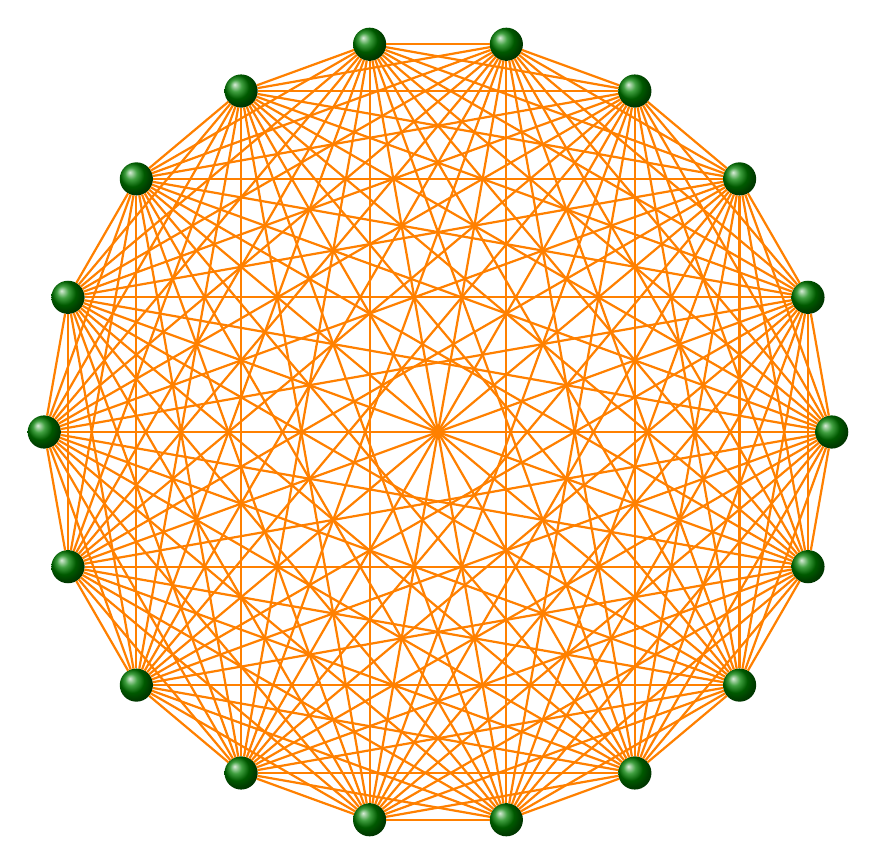
\begin{tikzpicture}
		\renewcommand*{\VertexBallColor}{green!50!black}
		\GraphInit[vstyle=Art]
		\grComplete[RA=5]{18}
		\end{tikzpicture}
	\end{center}
\end{titlepage}
\setcounter{page}{2}
\input{../Mod_base/copyright}
\tableofcontents 
%\addcontentsline{toc}{chapter}{\listtablename}
%\listoftables
\addcontentsline{toc}{chapter}{\listfigurename}
\listoffigures
\cleardoublepage\renewcommand\lstlistlistingname{Elenco esempi}
\addcontentsline{toc}{chapter}{\lstlistlistingname}
\addcontentsline{toc}{section}{Esempi}
\lstlistoflistings{}
\tcblistof[\section*]{thm}{Esempi}
\addcontentsline{toc}{section}{Contro esempi}
\tcblistof[\section*]{cthm}{Contro esempi}
\mainmatter%
%\opt{prima}{\input{primo/prima}}
%\opt{secondo}{\input{secondo/secondo}}
\chapter{Notazione scientifica}
\label{cha:Notazionescietifica}
 
\section{Conversioni}


\begin{esempiot}{Da decimale a esponenziale}{decexp1}
	Convertire il numero \num{0.0035} in notazione scientifica
\end{esempiot}
La virgola va' spostata di tre posti verso destra per cui
\[\num{0.0035}=\num[scientific-notation=true]{0.0035}\]
\begin{esempiot}{Da decimale a esponenziale}{decexp2}
	Convertire il numero \num{7255.45} in notazione scientifica
\end{esempiot}
La virgola va' spostata di tre posti verso sinistra per cui
\[\num{7255.45}=\num[scientific-notation=true]{7255.45}\]
\tcbstartrecording

\begin{exercise}
	Convertire il numero \num{0.372} in notazione scientifica\index{Notazione!scientifica}
	\tcblower
	La virgola va' spostata di un posto verso destra per cui
	\[\num{0.372}=\num[scientific-notation=true]{0.372}\]
\end{exercise}
%\tcbstoprecording
%% \newpage
%\section{Soluzioni esercizi Notazione scientifica}
%\tcbinputrecords
\tcbstartrecording
\chapter{Numeri complessi}
\label{cha:numericomplessibase}
 \section{Il piano complesso}
% 24/02/2018 :: 17:21:26 ::  \tcbstartrecording
 \begin{exercise}
	Disegnare nel piano complesso\index{Piano!complesso} il numero $z=1+2\uimm$\index{Numero!complesso}
	\tcblower
	Disegnare nel piano complesso il numero $z=1+2\uimm$
	\begin{center}
		\includestandalone[width=.6\textwidth]{terzo/grafici/Piano_complesso_11}
		\captionof{figure}{Piano complesso}\label{fig:disegnopianocomplesso11}
	\end{center}
\end{exercise}
 \begin{exercise}
Disegnare nel piano complesso\index{Piano!complesso} il numero $z=2+3\uimm$\index{Numero!complesso}
\tcblower
Disegnare nel piano complesso il numero $z=2+3\uimm$
\begin{center}
\includestandalone[width=.6\textwidth]{terzo/grafici/Piano_complesso_01}
\captionof{figure}{Piano complesso}\label{fig:disegnopianocomplesso01}
\end{center}
 \end{exercise}
  \begin{exercise}
  	Disegnare nel piano complesso il numero $z=-4+2\uimm$
  	\tcblower
  	Disegnare nel piano complesso il numero $z=-4+2\uimm$
  	\begin{center}
  		\includestandalone[width=.6\textwidth]{terzo/grafici/Piano_complesso_02}
  		\captionof{figure}{Piano complesso}\label{fig:disegnopianocomplesso02}
  	\end{center}
  \end{exercise}

  \begin{exercise}
Disegnare nel piano complesso il numero $z=2-7\uimm$
	\tcblower
Disegnare nel piano complesso il numero $z=2-7\uimm$
	\begin{center}
		\includestandalone[width=.6\textwidth]{terzo/grafici/Piano_complesso_12}
		\captionof{figure}{Piano complesso}\label{fig:disegnopianocomplesso12}
	\end{center}
\end{exercise}
\begin{exercise}[no solution]
	Disegnare nel piano complesso il numero $z=1+2\uimm$
\end{exercise}
\begin{exercise}[no solution]
Disegnare nel piano complesso il numero $z=+2\uimm$
\end{exercise}
\begin{exercise}[no solution]
	Disegnare nel piano complesso il numero $z=1$
\end{exercise}
\begin{exercise}[no solution]
	Disegnare nel piano complesso il numero $z=-3+2\uimm$
\end{exercise}
\begin{exercise}[no solution]
	Disegnare nel piano complesso il numero $z=-\frac{1}{2}+4\uimm$
\end{exercise}
\begin{exercise}[no solution]
	Disegnare nel piano complesso il numero $z=-3-2\uimm$
\end{exercise}
\begin{exercise}[no solution]
	Disegnare nel piano complesso il numero $z=-3+\uimm$
\end{exercise}
%\begin{exercise}[no solution]
%	Disegnare nel piano complesso il numero $z=-4+2\uimm$
%\end{exercise}

% \tcbstoprecording
%% \newpage
% \section{Soluzioni il piano complesso}
% \tcbinputrecords

 \section{Opposto di un numero complesso}
%\tcbstartrecording
\begin{exercise}
	Trovare e disegnare l'opposto\index{Numero!complesso!opposto} di $z=1+2\uimm$
	\tcblower
	Trovare e disegnare l'opposto di $z=1+2\uimm$
	
	L'opposto è $-z=-1-2\uimm$
	\begin{center}
		\includestandalone[width=.6\textwidth]{terzo/grafici/Piano_complesso_03}
		\captionof{figure}{Opposto di un complesso}\label{fig:disegnopianocomplesso03}
	\end{center}
\end{exercise}
\begin{exercise}[no solution]
	Trovare e disegnare l'opposto di $z=2+4\uimm$
\end{exercise}
\begin{exercise}
	Trovare e disegnare l'opposto di $z=3-2\uimm$
	\tcblower
	Trovare e disegnare l'opposto di $z=3-2\uimm$
	
	L'opposto è $z=-3+2\uimm$
	\begin{center}
		\includestandalone[width=.6\textwidth]{terzo/grafici/Piano_complesso_04}
		\captionof{figure}{Opposto di un complesso}\label{fig:disegnopianocomplesso04}
	\end{center}
\end{exercise}
\begin{exercise}
	Trovare e disegnare l'opposto di $z=1-2\uimm$
	\tcblower
	Trovare e disegnare l'opposto di $z=1-2\uimm$
	
	L'opposto è $z=-1+2\uimm$
	\begin{center}
		\includestandalone[width=.6\textwidth]{terzo/grafici/Piano_complesso_13}
		\captionof{figure}{Opposto di un complesso}\label{fig:disegnopianocomplesso13}
	\end{center}
\end{exercise}

\begin{exercise}[no solution]
	Trovare e disegnare l'opposto di  $z=5-7\uimm$
\end{exercise}
\begin{exercise}
	Trovare e disegnare l'opposto di $z=-1-3\uimm$
	\tcblower
	Trovare e disegnare l'opposto di $z=-1-3\uimm$
	
	L'opposto è $z=1+3\uimm$
	\begin{center}
		\includestandalone[width=.6\textwidth]{terzo/grafici/Piano_complesso_14}
		\captionof{figure}{Opposto di un complesso}\label{fig:disegnopianocomplesso14}
	\end{center}
\end{exercise}
\begin{exercise}[no solution]
	Trovare e disegnare l'opposto di  $z=-1$
\end{exercise}
\begin{exercise}[no solution]
	Trovare e disegnare l'opposto di  $z=3\uimm$
\end{exercise}
\begin{exercise}[no solution]
	Trovare e disegnare l'opposto di  $z=1-4\uimm$
\end{exercise}
\begin{exercise}[no solution]
	Trovare e disegnare l'opposto di  $z=1+4\uimm$
\end{exercise}
%
\begin{exercise}[no solution]
	Trovare e disegnare l'opposto di $z=-2-4\uimm$
\end{exercise}
\begin{exercise}[no solution]
	Trovare e disegnare l'opposto di $z=-1+2\uimm$
\end{exercise}
\begin{exercise}[no solution]
	Trovare e disegnare l'opposto di  $z=-5+7\uimm$
\end{exercise}
\begin{exercise}[no solution]
	Trovare e disegnare l'opposto di  $z=1+3\uimm$
\end{exercise}
\begin{exercise}[no solution]
	Trovare e disegnare l'opposto di  $z=1$
\end{exercise}
\begin{exercise}[no solution]
	Trovare e disegnare l'opposto di  $z=-3\uimm$
\end{exercise}
\begin{exercise}[no solution]
	Trovare e disegnare l'opposto di  $z=-1+4\uimm$
\end{exercise}
\begin{exercise}[no solution]
	Trovare e disegnare l'opposto di  $z=-1-4\uimm$
\end{exercise}
 \section{Coniugato di un numero complesso}
%\tcbstartrecording
\begin{exercise}
	Trovare e disegnare il coniugato\index{Numero!complesso!coniugato} $\conj{z}$ di $z=1-2\uimm$
	\tcblower
	Trovare e disegnare il coniugato $\conj{z}$ di $z=1-2\uimm$
	
	$\conj{z}=1+2\uimm$
	\begin{center}
		\includestandalone[width=.6\textwidth]{terzo/grafici/Piano_complesso_05}
		\captionof{figure}{Complesso coniugato}\label{fig:disegnopianocomplesso05}
	\end{center}
\end{exercise}
\begin{exercise}[no solution]
	Trovare e disegnare il coniugato $\conj{z}$ di $z=3+4\uimm$
\end{exercise}
\begin{exercise}[no solution]
	Trovare e disegnare il coniugato $\conj{z}$ di $z=-2+2\uimm$
\end{exercise}
\begin{exercise}[no solution]
	Trovare e disegnare il coniugato $\conj{z}$ di $z=-8+\uimm$
\end{exercise}
\begin{exercise}[no solution]
	Trovare e disegnare il coniugato $\conj{z}$ di $z=-3$
\end{exercise}
\begin{exercise}[no solution]
	Trovare e disegnare il coniugato $\conj{z}$ di $z=-2\uimm$
\end{exercise}
\begin{exercise}[no solution]
	Trovare e disegnare il coniugato $\conj{z}$ di $z=-3-8\uimm$
\end{exercise}
\begin{exercise}[no solution]
	Trovare e disegnare il coniugato $\conj{z}$ di $z=-2+5\uimm$
\end{exercise}
\begin{exercise}
	Trovare e disegnare il coniugato $\conj{z}$ di  $z=-1-2\uimm$
	\tcblower
	Trovare e disegnare il coniugato $\conj{z}$ di  $z=-1-2\uimm$
	
	$\conj{z}=-1+2\uimm$
	\begin{center}
		\includestandalone[width=.6\textwidth]{terzo/grafici/Piano_complesso_15}
		\captionof{figure}{Complesso coniugato}\label{fig:disegnopianocomplesso15}
	\end{center}
\end{exercise}
\begin{exercise}
	Trovare e disegnare il coniugato $\conj{z}$ di $z=-3-2\uimm$
	\tcblower
	Trovare e disegnare il coniugato $\conj{z}$ di $z=-3-2\uimm$
	
	$\conj{z}=-3+2\uimm$
	\begin{center}
		\includestandalone[width=.6\textwidth]{terzo/grafici/Piano_complesso_06}
		\captionof{figure}{Complesso coniugato}\label{fig:disegnopianocomplesso06}
	\end{center}
\end{exercise}
\begin{exercise}[no solution]
	Trovare e disegnare il coniugato $\conj{z}$ di $-3+4\uimm$
\end{exercise}
\section{Modulo di un numero complesso}
\begin{exercise}
	Trovare il modulo di $z=3+4\uimm$
	\tcblower
	Trovare il modulo di $z=3+4\uimm$
	$\norm{z}=\sqrt{9+16}=\sqrt{25}=5$
\end{exercise}
\begin{exercise}[no solution]
	Trovare il modulo di $z=-2+2\uimm$
\end{exercise}
\begin{exercise}[no solution]
	Trovare il modulo di $z=-8+\uimm$
\end{exercise}
\begin{exercise}[no solution]
	Trovare il modulo di $z=-3$
\end{exercise}
\begin{exercise}[no solution]
	Trovare il modulo di $z=-2\uimm$
\end{exercise}
 \begin{exercise}
	Trovare il modulo di $z=-3-8\uimm$
	\tcblower
	Trovare il modulo di $z=-3-8\uimm$
	$\norm{z}=\sqrt{9+64}=\sqrt{73}$
\end{exercise}
\begin{exercise}[no solution]
	Trovare il modulo di $z=-2+5\uimm$
\end{exercise}
%\tcbstoprecording
%% \newpage
% \section{Soluzioni coniugato di un numero complesso}
% \tcbinputrecords
 \tcbstoprecording
 \newpage
 \section{Soluzioni il piano complesso}
 \tcbinputrecords

 \section{Opposto di un numero complesso}
 %\tcbstartrecording
 \begin{exercise}
Trovare e disegnare l'opposto\index{Numero!complesso!opposto} di $z=1+2\uimm$
\tcblower
Trovare e disegnare l'opposto di $z=1+2\uimm$
\begin{center}
\includestandalone[width=.6\textwidth]{terzo/grafici/Piano_complesso_03}
\captionof{figure}{Opposto di un complesso}\label{fig:disegnopianocomplesso03}
\end{center}
 \end{exercise}
 \begin{exercise}[no solution]
 Trovare e disegnare l'opposto di $z=2+4\uimm$
 \end{exercise}
  \begin{exercise}
  Trovare e disegnare l'opposto di $z=3-2\uimm$
  	\tcblower
  	 Trovare e disegnare l'opposto di $z=3-2\uimm$
  	\begin{center}
  		\includestandalone[width=.6\textwidth]{terzo/grafici/Piano_complesso_04}
  		\captionof{figure}{Opposto di un complesso}\label{fig:disegnopianocomplesso04}
  	\end{center}
  \end{exercise}
 \begin{exercise}[no solution]
 	Trovare e disegnare l'opposto di $z=1-2\uimm$
 \end{exercise}
%\tcbstoprecording
%% \newpage
% \section{Soluzioni opposto del complesso}
% \tcbinputrecords
 
 \section{Coniugato di un numero complesso}
 %\tcbstartrecording
 \begin{exercise}
Trovare e disegnare il coniugato\index{Numero!complesso!coniugato} $\conj{z}$ di $z=1-2\uimm$
\tcblower
Trovare e disegnare il coniugato $\conj{z}$ di $z=1-2\uimm$

$\conj{z}=1+2\uimm$
\begin{center}
\includestandalone[width=.6\textwidth]{terzo/grafici/Piano_complesso_05}
\captionof{figure}{Complesso coniugato}\label{fig:disegnopianocomplesso05}
\end{center}
 \end{exercise}
 \begin{exercise}[no solution]
Trovare e disegnare il coniugato $\conj{z}$ di $z=-1-2\uimm$
 \end{exercise}
  \begin{exercise}
  Trovare e disegnare il coniugato $\conj{z}$ di $z=-3-2\uimm$
  	\tcblower
  	  Trovare e disegnare il coniugato $\conj{z}$ di $z=-3-2\uimm$
  	  
  	  $\conj{z}=-3+2\uimm$
  	\begin{center}
  		\includestandalone[width=.6\textwidth]{terzo/grafici/Piano_complesso_06}
  		\captionof{figure}{Complesso coniugato}\label{fig:disegnopianocomplesso06}
  	\end{center}
  \end{exercise}
 \begin{exercise}[no solution]
 		  Trovare e disegnare il coniugato $\conj{z}$ di $-3+4\uimm$
 \end{exercise}
%\tcbstoprecording
%% \newpage
% \section{Soluzioni coniugato di un numero complesso}
% \tcbinputrecords
 
\tcbstartrecording
\chapter{Operazioni con i numeri complessi}
 \section{Somma di due numeri complessi}
 %\tcbstartrecording
  \begin{exercise}[no solution]
 	Dati i numeri $z_1=-8-3\uimm$ e $z_2=4+6\uimm$, trovare la loro somma e  disegnare il numero nel piano complesso.
 \end{exercise}
 \begin{exercise}[no solution]
	Dati i numeri $z_1=-3-2\uimm$ e $z_2=1-6\uimm$, trovare la loro somma e  disegnare il numero nel piano complesso.
\end{exercise}
 \begin{exercise}
Dati i numeri $z_1=1-2\uimm$ e $z_2=3+4\uimm$, trovare la loro somma\index{Numero!complesso!somma} e  disegnare il numero nel piano complesso.
\tcblower
Dati i numeri $z_1=1-2\uimm$ e $z_2=3+4\uimm$, trovare la loro somma e  disegnare il numero nel piano complesso.
\[z_1+z_2=1=1-2\uimm+3+4\uimm=4+2\uimm \]
\begin{center}
\includestandalone[width=.6\textwidth]{terzo/grafici/Piano_complesso_07}
\captionof{figure}{Somma di numeri complessi}\label{fig:disegnopianocomplesso07}
\end{center}
 \end{exercise}
 \begin{exercise}[no solution]
Dati i numeri $z_1=-3+2\uimm$ e $z_2=1+6\uimm$, trovare la loro somma e  disegnare il numero nel piano complesso.
 \end{exercise}
 \begin{exercise}
 	Dati i numeri $z_1=-2+2\uimm$ e $z_2=-2-2\uimm$, trovare la loro somma e  disegnare il numero nel piano complesso.
 	\tcblower
 	Dati i numeri $z_1=-2+2\uimm$ e $z_2=-2-2\uimm$, trovare la loro somma e  disegnare il numero nel piano complesso.
 \[z_1+z_2=1=-2+2\uimm-2-2\uimm=-4\]
 	\begin{center}
 		\includestandalone[width=.6\textwidth]{terzo/grafici/Piano_complesso_08}
 		\captionof{figure}{Somma di numeri complessi}\label{fig:disegnopianocomplesso08}
 	\end{center}
 \end{exercise}
 \begin{exercise}
	Dati i numeri $z_1=-3+2\uimm$ e $z_2=1+6\uimm$, trovare la loro somma\index{Numero!complesso!somma} e  disegnare il numero nel piano complesso.
	\tcblower
	Dati i numeri $z_1=-3+2\uimm$ e $z_2=1+6\uimm$, trovare la loro somma e  disegnare il numero nel piano complesso.
	\[z_1+z_2=1=-3+2\uimm+1+6\uimm=-2+8\uimm \]
	\begin{center}
		\includestandalone[width=.6\textwidth]{terzo/grafici/Piano_complesso_16}
		\captionof{figure}{Somma di numeri complessi}\label{fig:disegnopianocomplesso16}
	\end{center}
\end{exercise}
 \begin{exercise}[no solution]
	Dati i numeri $z_1=-2+3\uimm$ e $z_2=6+1\uimm$, trovare la loro somma e  disegnare il numero nel piano complesso.
\end{exercise}
 \begin{exercise}[no solution]
	Dati i numeri $z_1=-5+3\uimm$ e $z_2=-4+\uimm$, trovare la loro somma e  disegnare il numero nel piano complesso.
\end{exercise}
 \begin{exercise}[no solution]
	Dati i numeri $z_1=+2\uimm$ e $z_2=-1+5\uimm$, trovare la loro somma e  disegnare il numero nel piano complesso.
\end{exercise}
 \begin{exercise}[no solution]
	Dati i numeri $z_1=-4+\uimm$ e $z_2=4+\uimm$, trovare la loro somma e  disegnare il numero nel piano complesso.
\end{exercise}
 \begin{exercise}[no solution]
	Dati i numeri $z_1=-3+2\uimm$ e $z_2=-3-2\uimm$, trovare la loro somma e  disegnare il numero nel piano complesso.
\end{exercise}
%\tcbstoprecording
%% \newpage
% \section{Soluzioni somma di due numeri complessi}
% \tcbinputrecords
  \section{Differenza di due numeri complessi}
 % \tcbstartrecording
 \begin{exercise}
 	Dati i numeri $z_1=2-3\uimm$ e $z_2=1-2\uimm$, trovare la loro differenza\index{Numero!complesso!differenza} e  disegnare il risultato  nel piano complesso.
 	\tcblower
 	Dati i numeri $z_1=-3-2\uimm$ e $z_2=-4-1\uimm$, trovare la loro differenza e  disegnare il risultato  nel piano complesso.
 	\[z_1-z_2=z_1=-3-2\uimm-(-4-1\uimm) =1+3\uimm \]
 	\begin{center}
 		\includestandalone[width=.6\textwidth]{terzo/grafici/Piano_complesso_09}
 		\captionof{figure}{Differenza di numeri complessi}\label{fig:disegnopianocomplesso09}
 	\end{center}
 \end{exercise}
 \begin{exercise}[no solution]
 	Dati i numeri $z_1=-3+2\uimm$ e $z_2=1+6\uimm$, trovare la loro differenza e  disegnare il risultato  nel piano complesso.
 \end{exercise}
 \begin{exercise}
 	Dati i numeri $z_1=3+2\uimm$ e $z_2=-4+\uimm$, trovare la loro differenza e  disegnare il risultato  nel piano complesso.
 	\tcblower
 	Dati i numeri $z_1=-2+2\uimm$ e $z_2=-2-2\uimm$, trovare la loro differenza e  disegnare il risultato  nel piano complesso.
 	\begin{center}
 		\includestandalone[width=.6\textwidth]{terzo/grafici/Piano_complesso_10}
 		\captionof{figure}{Differenza di numeri complessi}\label{fig:disegnopianocomplesso08a}
 	\end{center}
 \end{exercise}
 \begin{exercise}[no solution]
 	Dati i numeri $z_1=-3+2\uimm$ e $z_2=1+6\uimm$, trovare la loro differenza e  disegnare il risultato  nel piano complesso.
 \end{exercise}
 \section{Prodotto di numeri complessi}
%\tcbstartrecording
\begin{exercise}
	Eseguire\index{Numero!complesso!prodotto}la seguente moltiplicazione $(2-5\uimm)(3-4\uimm)$ fra numeri complessi.
	\tcblower
	Eseguire la seguente moltiplicazione $(2-5\uimm)(3-4\uimm)$ fra numeri complessi.
	\begin{align*}
	(2-5\uimm)(3-4\uimm)=&6-8\uimm-15\uimm-20\\
	=&-14-23\uimm
	\end{align*}
\end{exercise}
\begin{exercise}
	Eseguire la seguente moltiplicazione $(1-7\uimm)(1+5\uimm)$ fra numeri complessi.
	\tcblower
	Eseguire la seguente moltiplicazione $(1-7\uimm)(1+5\uimm)$ fra numeri complessi.
	\begin{align*}
	(1-7\uimm)(1+5\uimm)=&1+5\uimm-7\uimm-20\\
	=&36-2\uimm
	\end{align*}
\end{exercise}
\begin{exercise}
	Eseguire la seguente moltiplicazione $(1-5\uimm)(1+5\uimm) $ fra numeri complessi.
	\tcblower
	Eseguire la seguente moltiplicazione $(1-5\uimm)(1+5\uimm)$ fra numeri complessi.
	\begin{align*}
	(1-5\uimm)(1+5\uimm)=&1+5\uimm-5\uimm+25\\
	=&26
	\end{align*}
\end{exercise}
\begin{exercise}
	Eseguire la seguente moltiplicazione $(1-3\uimm)(6-2\uimm)(3+2\uimm)$ fra numeri complessi.
	\tcblower
	Eseguire la seguente moltiplicazione $(1-3\uimm)(6-2\uimm)(3+2\uimm)$ fra numeri complessi.
	\begin{align*}
	(1-3\uimm)(6-2\uimm)(3+2\uimm)=&(1-2\uimm-18\uimm-6)(3+2\uimm)\\
	=&-20\uimm(3+2\uimm)\\
	=&40-60\uimm\\
	\end{align*}
\end{exercise}

%\tcbstoprecording
%% \newpage
% \section{Soluzioni esercizi numeri complessi}
% \tcbinputrecords
 \section{Divisione di  numeri complessi}
%\tcbstartrecording
\begin{exercise}
	Eseguire\index{Numero!complesso!divisione}la seguente divisione $\dfrac{3-2\uimm}{1-5\uimm}$ fra numeri complessi.
	\tcblower
	Eseguire la seguente divisione  $\dfrac{3-2\uimm}{1-5\uimm}$ fra numeri complessi.
	\begin{align*}
	\dfrac{3-2\uimm}{1-5\uimm}=&\dfrac{3-2\uimm}{1-5\uimm}\dfrac{1+5\uimm}{1+5\uimm}\\
	=&\dfrac{3+15\uimm-2\uimm+10}{1+25}\\
	=&\dfrac{13+13\uimm}{26}\\
	=&\dfrac{13}{26}+\dfrac{13}{26}\uimm\\
	\end{align*}
\end{exercise}
\begin{exercise}
	Eseguire\index{Numero!complesso!divisione}la seguente divisione $\dfrac{5-2\uimm}{3+4\uimm}$ fra numeri complessi.
	\tcblower
	Eseguire la seguente divisione  $\dfrac{5-2\uimm}{3+4\uimm}$ fra numeri complessi.
	\begin{align*}
	\dfrac{5-2\uimm}{3+4\uimm}=&\dfrac{5-2\uimm}{3+4\uimm}\dfrac{3-4\uimm}{3-4\uimm}\\
	=&\dfrac{15-20\uimm-6\uimm-8}{9+16}\\
	=&\dfrac{7-26\uimm}{9+16}\\
	=&\dfrac{7}{25}-\dfrac{26}{25}\uimm\\
	\end{align*}
\end{exercise}
\begin{exercise}
	Eseguire le seguenti operazioni  $\dfrac{1-\uimm}{3\uimm}\dfrac{5-6\uimm}{1-\uimm}$ fra numeri complessi.
	\tcblower
	Eseguire le seguenti operazioni  $\dfrac{1-\uimm}{3\uimm}\dfrac{5-6\uimm}{1-\uimm}$ fra numeri complessi.
	\begin{align*}
	\dfrac{1-\uimm}{3\uimm}\dfrac{5-6\uimm}{1-\uimm}=&\dfrac{5-6\uimm-5\uimm-6}{3+3\uimm}\\
	=&\dfrac{-1-11\uimm}{3+3\uimm}\\
	=&\dfrac{-1-11\uimm}{3+3\uimm}\dfrac{3-3\uimm}{3-3\uimm}\\
	=&\dfrac{-3+3\uimm-33\uimm-33}{9+9}\\
	=&\dfrac{-36-30\uimm}{18}\\
	=&-2-\dfrac{5}{3}\uimm
	\end{align*}
\end{exercise}

\tcbstoprecording
 \newpage
 \section{Soluzioni esercizi numeri complessi}
 \tcbinputrecords
 \section{Differenza di due numeri complessi}
% \tcbstartrecording
 \begin{exercise}
Dati i numeri $z_1=2-3\uimm$ e $z_2=1-2\uimm$, trovare la loro differenza\index{Numero!complesso!differenza} e  disegnare il risultato  nel piano complesso.
\tcblower
Dati i numeri $z_1=-3-2\uimm$ e $z_2=-4-1\uimm$, trovare la loro differenza e  disegnare il risultato  nel piano complesso.
\[z_1-z_2=z_1=-3-2\uimm-(-4-1\uimm) =1+3\uimm \]
\begin{center}
\includestandalone[width=.6\textwidth]{terzo/grafici/Piano_complesso_09}
\captionof{figure}{Differenza di numeri complessi}\label{fig:disegnopianocomplesso09}
\end{center}
 \end{exercise}
 \begin{exercise}[no solution]
Dati i numeri $z_1=-3+2\uimm$ e $z_2=1+6\uimm$, trovare la loro differenza e  disegnare il risultato  nel piano complesso.
 \end{exercise}
 \begin{exercise}
 	Dati i numeri $z_1=3+2\uimm$ e $z_2=-4+\uimm$, trovare la loro differenza e  disegnare il risultato  nel piano complesso.
 	\tcblower
 	Dati i numeri $z_1=-2+2\uimm$ e $z_2=-2-2\uimm$, trovare la loro differenza e  disegnare il risultato  nel piano complesso.
 	\begin{center}
 		\includestandalone[width=.6\textwidth]{terzo/grafici/Piano_complesso_10}
 		\captionof{figure}{Differenza di numeri complessi}\label{fig:disegnopianocomplesso08a}
 	\end{center}
 \end{exercise}
 \begin{exercise}[no solution]
 	Dati i numeri $z_1=-3+2\uimm$ e $z_2=1+6\uimm$, trovare la loro differenza e  disegnare il risultato  nel piano complesso.
 \end{exercise}

%\tcbstoprecording
%% \newpage
% \section{Soluzioni differenza di due numeri complessi}
% \tcbinputrecords
 
 \section{Prodotto di  numeri complessi}
 %\tcbstartrecording
 \begin{exercise}
Eseguire\index{Numero!complesso!prodotto}la seguente moltiplicazione\[(2-5\uimm)(3-4\uimm) \] fra numeri complessi.
\tcblower
Eseguire la seguente moltiplicazione $(2-5\uimm)(3-4\uimm)$ fra numeri complessi.
\begin{align*}
(2-5\uimm)(3-4\uimm)=&6-8\uimm-15\uimm-20\\
=&-14-23\uimm
\end{align*}
 \end{exercise}
 \begin{exercise}
	Eseguire la seguente moltiplicazione\[(1-7\uimm)(1+5\uimm) \]fra numeri complessi.
	\tcblower
	Eseguire la seguente moltiplicazione $(1-7\uimm)(1+5\uimm)$ fra numeri complessi.
	\begin{align*}
	(1-7\uimm)(1+5\uimm)=&1+5\uimm-7\uimm-20\\
	=&36-2\uimm
	\end{align*}
\end{exercise}
 \begin{exercise}
	Eseguire la seguente moltiplicazione\[(1-5\uimm)(1+5\uimm) \] fra numeri complessi.
	\tcblower
	Eseguire la seguente moltiplicazione $(1-5\uimm)(1+5\uimm)$ fra numeri complessi.
	\begin{align*}
	(1-5\uimm)(1+5\uimm)=&1+5\uimm-5\uimm+25\\
	=&26
	\end{align*}
\end{exercise}
\begin{exercise}
	Eseguire la seguente moltiplicazione\[(1-3\uimm)(6-2\uimm)(3+2\uimm)\] fra numeri complessi.
	\tcblower
	Eseguire la seguente moltiplicazione $(1-3\uimm)(6-2\uimm)(3+2\uimm)$ fra numeri complessi.
	\begin{align*}
	(1-3\uimm)(6-2\uimm)(3+2\uimm)=&(1-2\uimm-18\uimm-6)(3+2\uimm)\\
	=&-20\uimm(3+2\uimm)\\
	=&40-60\uimm\\
	\end{align*}
\end{exercise}

%\tcbstoprecording
%% \newpage
% \section{Soluzioni esercizi numeri complessi}
% \tcbinputrecords
 
 \section{Divisione di  numeri complessi}
 %\tcbstartrecording
 \begin{exercise}
Eseguire\index{Numero!complesso!divisione}la seguente divisione \[\dfrac{3-2\uimm}{1-5\uimm} \] fra numeri complessi.
\tcblower
Eseguire la seguente divisione  $\dfrac{3-2\uimm}{1-5\uimm}$ fra numeri complessi.
\begin{align*}
\dfrac{3-2\uimm}{1-5\uimm}=&\dfrac{3-2\uimm}{1-5\uimm}\dfrac{1+5\uimm}{1+5\uimm}\\
=&\dfrac{3+15\uimm-2\uimm+10}{1+25}\\
=&\dfrac{13+13\uimm}{26}\\
=&\dfrac{13}{26}+\dfrac{13}{26}\uimm\\
\end{align*}
 \end{exercise}
 \begin{exercise}
	Eseguire\index{Numero!complesso!divisione}la seguente divisione \[\dfrac{5-2\uimm}{3+4\uimm} \] fra numeri complessi.
	\tcblower
	Eseguire la seguente divisione  $\dfrac{5-2\uimm}{3+4\uimm}$ fra numeri complessi.
	\begin{align*}
	\dfrac{5-2\uimm}{3+4\uimm}=&\dfrac{5-2\uimm}{3+4\uimm}\dfrac{3-4\uimm}{3-4\uimm}\\
	=&\dfrac{15-20\uimm-6\uimm-8}{9+16}\\
	=&\dfrac{7-26\uimm}{9+16}\\
	=&\dfrac{7}{25}-\dfrac{26}{25}\uimm\\
	\end{align*}
\end{exercise}
 \begin{exercise}
	Eseguire le seguenti operazioni  \[\dfrac{1-\uimm}{3\uimm}\dfrac{5-6\uimm}{1-\uimm}\] fra numeri complessi.
	\tcblower
	Eseguire le seguenti operazioni  $\dfrac{1-\uimm}{3\uimm}\dfrac{5-6\uimm}{1-\uimm}$ fra numeri complessi.
	\begin{align*}
	\dfrac{1-\uimm}{3\uimm}\dfrac{5-6\uimm}{1-\uimm}=&\dfrac{5-6\uimm-5\uimm-6}{3+3\uimm}\\
	=&\dfrac{-1-11\uimm}{3+3\uimm}\\
	=&\dfrac{-1-11\uimm}{3+3\uimm}\dfrac{3-3\uimm}{3-3\uimm}\\
	=&\dfrac{-3+3\uimm-33\uimm-33}{9+9}\\
	=&\dfrac{-36-30\uimm}{18}\\
	=&-2-\dfrac{5}{3}\uimm
	\end{align*}
\end{exercise}

\tcbstoprecording
% \newpage
 \section{Soluzioni esercizi numeri complessi}
 \tcbinputrecords
 
\section{Modulo e argomento}
\begin{esempiot}{Trovare modulo ed argomento di un numero complesso}{numcomarg1}\index{Numero!complesso!modulo}\index{Numero!complesso!argomento}
	Dato  il numero complesso \[z=2+3\uimm\] determinarne modulo $\abs{z}$ ed l'argomento $\phi$ con $\ang{0}\leq\phi<\ang{360}$
\end{esempiot}
Rappresento il numero complesso nel piano di Gauss
\begin{center}
	\includestandalone[width=.6\textwidth]{terzo/grafici/argomentocomplesso1}
	\captionof{figure}{Modulo ed argomento uno}\label{fig:moduloargomentouno}
\end{center}
Formule coinvolte:
\begin{align*}
\abs{z}=&\sqrt{a^2+b^2}\\
\phi=&\arctan\left(\dfrac{b}{a}\right)
\end{align*}
Quindi per il modulo
\begin{align*}
z=&2+3\uimm\\
\abs{z}=&\sqrt{2^2+3^2}\\
=&\sqrt{4+9}\\
=&\sqrt{13}\\
\simeq&\num[round-precision=\lungarrotandamento,round-mode=places]{3.6055551275}
\end{align*}
Utilizzando la calcolatrice
 \begin{center}
	\begin{tabular}{ll}
		\tasto{2}\tastoquadrato\tastopiu\tasto{3}\tastoquadrato\tastouguale&13\\
	\tastoradicequadrata\tastoans\tastouguale&$\simeq\num[round-precision=\lungarrotandamento,round-mode=places]{3.6055551275}$
		\end{tabular}
\end{center}
Per l'argomento

Verifico la calcolatrice \testgradi
\begin{align*}
z=&2+3\uimm\\
\phi=&\arctan\left(\dfrac{3}{2}\right)\\
\simeq&\ang[round-precision=\lungarrotandamento,round-mode=places]{56.30993247}
\end{align*}
Utilizzando la calcolatrice
\begin{center}
	\begin{tabular}{ll}
		\tasto{3}\tastodiv\tasto{2}\tastouguale&1.5\\
\tastoitan\tastoans\tastouguale&$\simeq\ang[round-precision=\lungarrotandamento,round-mode=places]{56.30993247}$
	\end{tabular}
\end{center}

\begin{esempiot}{Trovare modulo ed l'argomento di un numero complesso}{}
	Dato  il numero complesso \[z=-2+3\uimm\] determinarne modulo $\abs{z}$ ed argomento $\phi$ con $\ang{0}\leq\phi<\ang{360}$
\end{esempiot}
Rappresento il numero complesso nel piano di Gauss
\begin{center}
	\includestandalone[width=0.6\textwidth]{terzo/grafici/argomentocomplesso2}
	\captionof{figure}{Modulo ed argomento due}\label{fig:moduloargomentodue}
\end{center}
Formule coinvolte:
\begin{align*}
\abs{z}=&\sqrt{a^2+b^2}\\
\phi=&\arctan\left(\dfrac{b}{a}\right)
\end{align*}
Quindi per il modulo
\begin{align*}
z=&-2+3\uimm\\
\abs{z}=&\sqrt{(-2)^2+3^2}\\
=&\sqrt{4+9}\\
=&\sqrt{13}\\
\simeq&\num[round-precision=\lungarrotandamento,round-mode=places]{3.6055551275}
\end{align*}
Utilizzando la calcolatrice
\begin{center}
	\begin{tabular}{ll}
		\tastoparentesisin\tasto{-2}\tastoparentesides\tastoquadrato\tastopiu\tasto{3}\tastoquadrato\tastouguale&13\\
		\tastoradicequadrata\tastoans\tastouguale&$\simeq\num[round-precision=\lungarrotandamento,round-mode=places]{3.6055551275}$
	\end{tabular}
\end{center}
Per l'argomento

Verifico la calcolatrice \testgradi
\begin{align*}
z=&-2+3\uimm\\
\phi=&\arctan\left(-\dfrac{3}{2}\right)\\
\simeq&\ang[round-precision=\lungarrotandamento,round-mode=places]{-56.30993247}
\intertext{Correggo}
\simeq&\ang{180}\ang[round-precision=\lungarrotandamento,round-mode=places]{-56.30993247}\\
\simeq&\ang[round-precision=\lungarrotandamento,round-mode=places]{123.6900675}
\end{align*}
Utilizzando la calcolatrice
\begin{center}
	\begin{tabular}{ll}
		\tasto{3}\tastodiv\tastoparentesisin\tasto{-2}\tastoparentesides\tastouguale&\num{-1.5}\\
		\tastoitan\tastoans\tastouguale&$\simeq\ang[round-precision=\lungarrotandamento,round-mode=places]{-56.30993247}$\\
		\tasto{180}\tastopiu\tastoans\tastouguale&$\simeq\ang[round-precision=\lungarrotandamento,round-mode=places]{123.6900675}$
	\end{tabular}
\end{center}
\begin{esempiot}{Trovare modulo ed l'argomento di un numero complesso}{}
	Dato  il numero complesso \[z=-2-3\uimm\] determinarne modulo $\abs{z}$ ed argomento $\phi$ con $\ang{0}\leq\phi<\ang{360}$
\end{esempiot}
Rappresento il numero complesso nel piano di Gauss
\begin{center}
	\includestandalone[width=.6\textwidth]{terzo/grafici/argomentocomplesso3}
	\captionof{figure}{Modulo ed argomento tre}\label{fig:moduloargomentotre}
\end{center}
Formule coinvolte:
\begin{align*}
\abs{z}=&\sqrt{a^2+b^2}\\
\phi=&\arctan\left(\dfrac{b}{a}\right)
\end{align*}
Quindi per il modulo
\begin{align*}
z=&-2-3\uimm\\
\abs{z}=&\sqrt{(-2)^2+(-3)^2}\\
=&\sqrt{4+9}\\
=&\sqrt{13}\\
\simeq&\num[round-precision=\lungarrotandamento,round-mode=places]{3.6055551275}
\end{align*}
Utilizzando la calcolatrice
\begin{center}
	\begin{tabular}{ll}
		\tastoparentesisin\tasto{-2}\tastoparentesides\tastoquadrato\tastopiu\tastoparentesisin\tasto{-3}\tastoparentesides\tastoquadrato\tastouguale&13\\
		\tastoradicequadrata\tastoans\tastouguale&$\simeq\num[round-precision=\lungarrotandamento,round-mode=places]{3.6055551275}$
	\end{tabular}
\end{center}
Per l'argomento

Verifico la calcolatrice \testgradi
\begin{align*}
z=&-2-3\uimm\\
\phi=&\arctan\left(\dfrac{-3}{-2}\right)\\
\simeq&\ang[round-precision=\lungarrotandamento,round-mode=places]{56.30993247}
\intertext{correggo}
\simeq&\ang{180}+\ang[round-precision=\lungarrotandamento,round-mode=places]{56.30993247}\\
\simeq&\ang[round-precision=\lungarrotandamento,round-mode=places]{236.30993247}
\end{align*}
Utilizzando la calcolatrice
\begin{center}
	\begin{tabular}{ll}
		\tasto{-3}\tastodiv\tasto{-2}\tastouguale&1.5\\
		\tastoitan\tastoans\tastouguale&$\simeq\ang[round-precision=\lungarrotandamento,round-mode=places]{56.30993247}$\\
		\tasto{180}\tastopiu\tastoans\tastouguale&$\simeq\ang[round-precision=\lungarrotandamento,round-mode=places]{236.3099325}$\\
	\end{tabular}
\end{center}

\begin{esempiot}{Trovare modulo ed l'argomento di un numero complesso}{}
	Dato  il numero complesso \[z=2-3\uimm\] determinarne modulo $\abs{z}$ ed argomento $\phi$ con $\ang{0}\leq\phi<\ang{360}$
\end{esempiot}
Rappresento il numero complesso nel piano di Gauss
\begin{center}
	\includestandalone[width=.6\textwidth]{terzo/grafici/argomentocomplesso4}
	\captionof{figure}{Modulo ed argomento quattro}\label{fig:moduloargomentoquattro}
\end{center}
Formule coinvolte:
\begin{align*}
\abs{z}=&\sqrt{a^2+b^2}\\
\phi=&\arctan\left(\dfrac{b}{a}\right)
\end{align*}
Quindi per il modulo
\begin{align*}
z=&2-3\uimm\\
\abs{z}=&\sqrt{2^2+(-3)^2}\\
=&\sqrt{4+9}\\
=&\sqrt{13}\\
\simeq&\num[round-precision=\lungarrotandamento,round-mode=places]{3.6055551275}
\end{align*}
Utilizzando la calcolatrice
\begin{center}
	\begin{tabular}{ll}
		\tasto{2}\tastoquadrato\tastopiu\tastoparentesisin\tasto{-3}\tastoparentesides\tastoquadrato\tastouguale&13\\
		\tastoradicequadrata\tastoans\tastouguale&$\simeq\num[round-precision=\lungarrotandamento,round-mode=places]{3.6055551275}$
	\end{tabular}
\end{center}
Per l'argomento

Verifico la calcolatrice \testgradi
\begin{align*}
z=&2-3\uimm\\
\phi=&\arctan\left(\dfrac{-3}{2}\right)\\
\simeq&\ang[round-precision=\lungarrotandamento,round-mode=places]{-56.30993247}
\intertext{correggo}
\simeq&\ang{360}\ang[round-precision=\lungarrotandamento,round-mode=places]{-56.30993247}\\
\simeq&\ang[round-precision=\lungarrotandamento,round-mode=places]{303.6900675}
\end{align*}
Utilizzando la calcolatrice
\begin{center}
	\begin{tabular}{ll}
		\tasto{-3}\tastodiv\tasto{2}\tastouguale&-1.5\\
		\tastoitan\tastoans\tastouguale&$\simeq\ang[round-precision=\lungarrotandamento,round-mode=places]{-56.30993247}$\\
			\tasto{360}\tastopiu\tastoans\tastouguale&$\simeq\ang[round-precision=\lungarrotandamento,round-mode=places]{303.6900675}$\\
		\end{tabular}
\end{center}
\chapter{Angoli}
\label{cha:angolibase}

\section{Conversioni radianti gradi}
\begin{esempiot}{Conversioni radianti gradi}{}
Convertire $\alpha=\ang{45;58;25}$ in radianti\index{Radianti}
\end{esempiot}
Prima convertiamo in gradi decimali\index{Radianti}\index{Grado!Sessagesimale}
\[\alpha=\ang{45}+\left(\dfrac{58}{60}\right)^{\si{\degree} }+\left(\dfrac{25}{3600}\right)^{\si{\degree} }=\ang{45}+\left(\dfrac{58\cdot60+25}{3600}\right)^{\si{\degree} } =\ang{45}+\left(\dfrac{3505}{3600}\right)^{\si{\degree} }\approx\ang[round-precision=\lungarrotandamento,round-mode=places]{45.97361111}\]
\[\rho=\dfrac{\pi}{180}\alpha\approx\dfrac{\pi}{180}\cdot\ang[round-precision=\lungarrotandamento,round-mode=places]{45.97361111}\approx\SI[round-precision=\lungarrotandamento,round-mode=places]{0.802390882}{\radian}\]
\stampapuntini
\begin{esempiot}{Conversioni radianti gradi}{}
	Convertire $\alpha=\ang{70;48;25}$ in radianti
\end{esempiot}
Prima convertiamo in gradi decimali \index{Radiante}\index{Grado!Sessagesimale}\index{Grado!Sessadecimale}
\[\alpha=\puntini{\ang{70}}+\left(\dfrac{48}{60}\right)^{\si{\degree} }+\left(\dfrac{25}{3600}\right)^{\si{\degree} }=\ang{70}+\left(\dfrac{\puntini{48\cdot60}+25}{3600}\right)^{\si{\degree} } =\ang{70}+\left(\dfrac{\puntini{2905}}{3600}\right)^{\si{\degree} }\approx\ang[round-precision=\lungarrotandamento,round-mode=places]{70.806944}\]
\[\rho=\dfrac{\puntini{\pi}}{180}\alpha\approx\dfrac{\puntini{\pi}}{180}\cdot\ang[round-precision=\lungarrotandamento,round-mode=places]{70.806944}\approx\puntini{\SI[round-precision=\lungarrotandamento,round-mode=places]{1.2358143}{\radian}}\]
\nonstampapuntini
\begin{esempiot}{Conversioni radianti gradi}{}
	Convertire\SI[round-precision=\lungarrotandamento,round-mode=places]{2.856}{\radian} in gradi sessagesimali
\end{esempiot}
\[\alpha=\dfrac{180}{\pi}\cdot\rho=\dfrac{180}{\pi}\cdot\SI[round-precision=\lungarrotandamento,round-mode=places]{2.856}{\radian}\approx\ang[round-precision=\lungarrotandamento,round-mode=places]{163.6367463}\]
Iniziamo con 
$\alpha=\ang{163}+\ang[round-precision=\lungarrotandamento,round-mode=places]{0.6367463}$
\begin{align*}
\alpha^{\si{\degree} }&=\ang{163}\\ 
\alpha^{\si{\arcminute}}&=\ang[round-precision=\lungarrotandamento,round-mode=places]{0.6367463;;}\cdot 60=\ang[round-precision=\lungarrotandamento,round-mode=places]{;38.20477736;}=\ang{;38;}\\
\alpha^{\si{\arcsecond}}&=\ang[round-precision=\lungarrotandamento,round-mode=places]{;0.204777358;}\cdot 60\approx\ang{;;12}\\
\end{align*}
abbiamo quindi
\[\alpha=\ang[round-precision=\lungarrotandamento,round-mode=places]{163.6367463}=\ang{163;38;12}\]
\stampapuntini
\begin{esempiot}{Conversioni radianti gradi}{}
	Convertire \SI[round-precision=\lungarrotandamento,round-mode=places]{0.823310}{\radian} in gradi sessagesimali
\end{esempiot}
\[\alpha=\dfrac{180}{\pi}\cdot\rho=\dfrac{180}{\pi}\cdot\SI[round-precision=\lungarrotandamento,round-mode=places]{0.823310}{\radian}\approx\puntini{\ang[round-precision=\lungarrotandamento,round-mode=places]{47.17218823}}\]
Iniziamo con 
$\alpha=\ang{47}+\ang[round-precision=\lungarrotandamento,round-mode=places]{0.17218823}$
\begin{align*}
\alpha^{\si{\degree}}&=\puntini{\ang{47}}\\ 
\alpha^{\si{\arcminute}}&=\ang[round-precision=\lungarrotandamento,round-mode=places]{0.17218823;;}\cdot 60=\puntini{\ang[round-precision=\lungarrotandamento,round-mode=places]{;10.33129385;}}=\puntini{\ang{;10;}}\\
\alpha^{\si{\arcsecond}}&=\puntini{\ang[round-precision=\lungarrotandamento,round-mode=places]{;0.331293854;}\cdot 60\approx\ang{;;19}}\\
\end{align*}
abbiamo quindi
\[\alpha=\ang[round-precision=\lungarrotandamento,round-mode=places]{47.17218823}=\ang{47;10;19}\]
\section{Da grado sessagesimale a sessa-decimale}
 \tcbstartrecording
 \begin{exercise}
Trasformare $\alpha=\ang{52;38;28}$ in forma sessa-decimale\index{Grado!Sessadecimale}\index{Grado!Sessagesimale}
\tcblower
\begin{align*}
\alpha=&\ang{52}+\left(\dfrac{38}{60}\right)^{\si{\degree} }+\left(\dfrac{28}{3600}\right)^{\si{\degree} }\\
=&\ang{52}+\left(\dfrac{38\cdot60+28}{3600}\right)^{\si{\degree} }\\
=&\ang{52}+\left(\dfrac{2308}{3600}\right)^{\si{\degree} }\approx\ang[round-precision=\lungarrotandamento,round-mode=places]{52,641111}
\end{align*}
\end{exercise}
 \begin{exercise}
 	Trasformare  $\alpha=\ang{75;55;35}$ in forma sessa-decimale\index{Grado!Sessadecimale}\index{Grado!Sessagesimale}
 	\tcblower
 	\begin{align*}
 	\alpha=&\ang{75}+\left(\dfrac{55}{60}\right)^{\si{\degree} }+\left(\dfrac{35}{3600}\right)^{\si{\degree} }\\
 	=&\ang{75}+\left(\dfrac{55\cdot60+35}{3600}\right)^{\si{\degree}}\\
 	=&\ang{75}+\left(\dfrac{3335}{3600}\right)^{\si{\degree}}\approx\ang[round-precision=\lungarrotandamento,round-mode=places]{75,92638}
 	\end{align*}
 \end{exercise}
  \begin{exercise}
  	Trasformare  $\alpha=\ang{38;21;10}$ in forma sessa-decimale\index{Grado!Sessadecimale}\index{Grado!Sessagesimale}
  	\tcblower
  	\begin{align*}
  	\alpha=&\ang{38}+\left(\dfrac{21}{60}\right)^{\si{\degree} }+\left(\dfrac{10}{3600}\right)^{\si{\degree} }\\
  	=&\ang{38}+\left(\dfrac{21\cdot60+10}{3600}\right)^{\si{\degree}}\\
  	=&\ang{38}+\left(\dfrac{1270}{3600}\right)^{\si{\degree}}\approx\ang[round-precision=\lungarrotandamento,round-mode=places]{38,35277778}
  	\end{align*}
  \end{exercise}
  \begin{exercise}
  	Trasformare  $\alpha=\ang{74;58;27}$ in forma sessa-decimale\index{Grado!Sessadecimale}\index{Grado!Sessagesimale}
  	\tcblower
  	\begin{align*}
  	\alpha=&\ang{74}+\left(\dfrac{58}{60}\right)^{\si{\degree} }+\left(\dfrac{27}{3600}\right)^{\si{\degree} }\\
  	=&\ang{74}+\left(\dfrac{58\cdot60+27}{3600}\right)^{\si{\degree}}\\
  	=&\ang{74}+\left(\dfrac{3507}{3600}\right)^{\si{\degree}}\approx\ang[round-precision=\lungarrotandamento,round-mode=places]{74,9741666667}
  	\end{align*}
  \end{exercise}
  \begin{exercise}
  	Trasformare  $\alpha=\ang{128;31;5}$ in forma sessa-decimale\index{Grado!Sessadecimale}\index{Grado!Sessagesimale}
  	\tcblower
  	\begin{align*}
  	\alpha=&\ang{128}+\left(\dfrac{31}{60}\right)^{\si{\degree} }+\left(\dfrac{5}{3600}\right)^{\si{\degree} }\\
  	=&\ang{128}+\left(\dfrac{31\cdot60+5}{3600}\right)^{\si{\degree}}\\
  	=&\ang{128}+\left(\dfrac{1865}{3600}\right)^{\si{\degree}}\approx\ang[round-precision=\lungarrotandamento,round-mode=places]{128,51666600667}
  	\end{align*}
  \end{exercise}
  \begin{exercise}
  	Trasformare  $\alpha=\ang{77;40;10}$ in forma sessa-decimale\index{Grado!Sessadecimale}\index{Grado!Sessagesimale}
  	\tcblower
  	\begin{align*}
  	\alpha=&\ang{77}+\left(\dfrac{40}{60}\right)^{\si{\degree} }+\left(\dfrac{10}{3600}\right)^{\si{\degree} }\\
  	=&\ang{77}+\left(\dfrac{40\cdot60+10}{3600}\right)^{\si{\degree}}\\
  	=&\ang{77}+\left(\dfrac{2410}{3600}\right)^{\si{\degree}}\approx\ang[round-precision=\lungarrotandamento,round-mode=places]{77,66944444}
  	\end{align*}
  \end{exercise}
\tcbstoprecording
\newpage
\section{Soluzioni da grado sessagesimale a sessa-decimale}
\tcbinputrecords
\section{Da grado sessadecimale a sessagesimale}
\tcbstartrecording
\begin{exercise}
	Convertire $\alpha=\ang{75.84}$ in gradi sessagesimali\index{Grado!Sessadecimale}\index{Grado!Sessagesimale}
	\tcblower
	Iniziamo con\index{Grado!Sessadecimale}\index{Grado!Sessagesimale}
	$\alpha=\ang{75}+\ang{0.84}$ in gradi sessagesimali
	\begin{align*}
	\alpha^{\si{\degree}}&=\ang{75}\\ 
	\alpha^{\si{\arcminute}}&=\ang{0.84}\cdot 60=\ang{;50.4;}=\ang{;50;}\\
	\alpha^{\si{\arcsecond}}&=\ang{;0.4;}\cdot 60=\ang{;;24}\\
	\end{align*}
	abbiamo quindi
	\[\alpha=\ang{75.84}=\ang{75;50;24}\]
\end{exercise}
\begin{exercise}
Convertire $\alpha=\ang{45.35}$ in gradi sessagesimali\index{Grado!Sessadecimale}\index{Grado!Sessagesimale}
	\tcblower
Iniziamo con 
$\alpha=\ang{45}+\ang{0.35}$
\begin{align*}
\alpha^{\si{\degree}}&=\ang{45}\\ 
\alpha^{\si{\arcminute}}&=\ang{0.35}\cdot 60=\ang{;21.0;}=\ang{;21;}\\
\alpha^{\si{\arcsecond}}&=\ang{;0;}\cdot 60=\ang{;;0}\\
\end{align*}
abbiamo quindi
\[\alpha=\ang{45.35}=\ang{45;21;0}\]
\end{exercise}
\begin{exercise}
	Convertire $\alpha=\ang{74.9742}$ in gradi sessagesimali\index{Grado!Sessadecimale}\index{Grado!Sessagesimale}
	\tcblower
	Iniziamo con 
	$\alpha=\ang{74}+\ang{0.9742}$
	\begin{align*}
	\alpha^{\si{\degree}}&=\ang{74}\\ 
	\alpha^{\si{\arcminute}}&=\ang{0.9742}\cdot 60=\ang{;58.452;}\\
	\alpha^{\si{\arcsecond}}&=\ang{;0.452;}\cdot 60=\ang{;;27.12}\\
	\end{align*}
	abbiamo quindi
	\[\alpha=\ang{74.9742}=\ang{74;58;27}\]
\end{exercise}
\begin{exercise}
	Convertire $\alpha=\ang{128.5167}$ in gradi sessagesimali\index{Grado!Sessadecimale}\index{Grado!Sessagesimale}
	\tcblower
	Iniziamo con 
	$\alpha=\ang{128}+\ang{0.5167}$
	\begin{align*}
	\alpha^{\si{\degree}}&=\ang{128}\\ 
	\alpha^{\si{\arcminute}}&=\ang{0.5167}\cdot 60=\ang{;31.002;}\\
	\alpha^{\si{\arcsecond}}&=\ang{;0.002;}\cdot 60=\ang{;;0.12}\\
	\end{align*}
	abbiamo quindi
	\[\alpha=\ang{128.5167}=\ang{128;31;0}\]
\end{exercise}
\begin{exercise}
	Convertire $\alpha=\ang{77.6694}$ in gradi sessagesimali\index{Grado!Sessadecimale}\index{Grado!Sessagesimale}
	\tcblower
	Iniziamo con 
	$\alpha=\ang{77}+\ang{0.6694}$
	\begin{align*}
	\alpha^{\si{\degree}}&=\ang{77}\\ 
	\alpha^{\si{\arcminute}}&=\ang{0.6694}\cdot 60=\ang{;40.164;}\\
	\alpha^{\si{\arcsecond}}&=\ang{;0.164;}\cdot 60=\ang{;;9.84}\\
	\end{align*}
	abbiamo quindi
	\[\alpha=\ang{77.6694}=\ang{77;40;9}\]
\end{exercise}
\tcbstoprecording
\newpage
\section{Soluzioni da grado sessadecimale a sessagesimale}
\tcbinputrecords
\chapter{Goniometria}
\label{cha:goniometriaEss}
\section{Trovare seno coseno e tangente}\index{Seno}\index{Coseno}\index{Tangente}
\begin{esempiot}{Trovare seno coseno e tangente}{exemplum1}
	Se $\sin\alpha=\dfrac{3}{5}$ con $\dfrac{\pi}{2}\leq\alpha\leq\pi$ determinare coseno e tangente.
\end{esempiot}
Se $\sin\alpha=\dfrac{3}{5}$ disegno la figura\nobs\vref{fig:esempio1}. Con il vincolo $\dfrac{\pi}{2}\leq\alpha\leq\pi$ il Punto $P$ è nel secondo quadrante, di conseguenza il coseno è negativo, come è negativa la tangente.
\begin{align*}
\sin\alpha&=\dfrac{3}{5}\\
\cos\alpha&=-\sqrt{1-\sin^2\alpha}=\\
&=-\sqrt{1-\dfrac{9}{25}}=\\
&=-\sqrt{\dfrac{25-9}{25}}=\\
&=-\sqrt{\dfrac{16}{25}}=\\
&=-\dfrac{4}{5}\\
\end{align*}
Di conseguenza la tangente è:
\[\tan\alpha=\dfrac{\sin\alpha}{\cos\alpha}=\dfrac{\dfrac{3}{5}}{-\dfrac{4}{5}}=\dfrac{3}{5}\cdot\left(-\dfrac{5}{4}\right)=-\dfrac{3}{4}\]
\begin{esempiot}{Trovare seno coseno e tangente}{}\index{Seno}\index{Coseno}\index{Tangente}
	Se $cos\alpha=\dfrac{7}{9}$ con $\dfrac{3\pi}{2}\leq\alpha\leq 2\pi$ determinare seno e tangente.
\end{esempiot}
L'angolo è nel quarto quadrante come lo mostra la figura\nobs\vref{fig:esempio2}, quindi seno e tangente sono negativi
\begin{align*}
\cos\alpha&=\dfrac{7}{9}\\
\sin\alpha&=-\sqrt{1-\cos^2\alpha}=\\
&=-\sqrt{1-\dfrac{49}{81}}=\\
&=-\sqrt{\dfrac{81-49}{81}}=\\
&=-\sqrt{\dfrac{32}{81}}=\\
&=-\dfrac{4\sqrt{2}}{9}\\
\end{align*}
\[\tan\alpha=\dfrac{\sin\alpha}{\cos\alpha}=\dfrac{-\dfrac{4\sqrt{2}}{9}}{\dfrac{7}{9}}=-\dfrac{4\sqrt{2}}{9}\cdot\dfrac{9}{7}=-\dfrac{4\sqrt{2}}{7}\]
\begin{esempiot}{Trovare seno coseno e tangente}{}\index{Seno}\index{Coseno}\index{Tangente}
	Se $sin\alpha=-\dfrac{9}{10}$ con $\pi\leq\alpha\leq\frac{3\pi}{2}$ determinare coseno e tangente.
\end{esempiot}
Se $\sin\alpha=-\dfrac{9}{10}$ disegno la figura\nobs\vref{fig:esempio3}. Con il vincolo $\pi\leq\alpha\leq\dfrac{3\pi}{2}$ il punto $P$ è nel terzo quadrante, di conseguenza il coseno è negativo, mentre  la tangente è positiva.
\begin{align*}
\sin\alpha&=-\dfrac{9}{10}\\
\cos\alpha&=-\sqrt{1-\sin^2\alpha}=\\
&=-\sqrt{1-\dfrac{81}{100}}=\\
&=-\sqrt{\dfrac{100-81}{100}}=\\
&=-\sqrt{\dfrac{19}{100}}=\\
&=-\dfrac{\sqrt{19}}{100}\\
\end{align*}
Di conseguenza la tangente è:
\[\tan\alpha=\dfrac{\sin\alpha}{\cos\alpha}=\dfrac{-\dfrac{9}{10}}{-\dfrac{\sqrt{19}}{10}}=\left(-\dfrac{9}{10}\right)\cdot\left(-\dfrac{\sqrt{19}}{10}\right)=\dfrac{9}{\sqrt{19}}=\dfrac{9\sqrt{19}}{19}\]
\begin{esempiot}{Trovare seno coseno e tangente}{}\index{Seno}\index{Coseno}\index{Tangente}
	Se $cos\alpha=-\dfrac{5}{6}$ con $\dfrac{\pi}{2}\leq\alpha\leq \pi$ determinare seno e tangente.
\end{esempiot}
L'angolo è nel secondo quadrante come lo mostra la figura\nobs\vref{fig:esempio4}, quindi seno è positivo e la tangente è negativa
\begin{align*}
\cos\alpha&=-\dfrac{5}{6}\\
\sin\alpha&=\sqrt{1-\cos^2\alpha}=\\
&=\sqrt{1-\dfrac{25}{36}}=\\
&=\sqrt{\dfrac{36-25}{36}}=\\
&=\sqrt{\dfrac{11}{36}}=\\
&=\dfrac{\sqrt{11}}{6}\\
\end{align*}
\[\tan\alpha=\dfrac{\sin\alpha}{\cos\alpha}=\dfrac{\dfrac{\sqrt{11}}{6}}{-\dfrac{5}{6}}=\dfrac{\sqrt{11}}{6}\cdot\left(-\dfrac{6}{5}\right)=-\dfrac{\sqrt{11}}{5}\]
\begin{figure}
\begin{subfigure}[b]{.5\linewidth}
\centering
\includestandalone[width=.8\textwidth]{terzo/grafici/EquaElementareSeno1}
\captionsetup{format=esempio}
\caption{Seno noto}\label{fig:esempio1}
\end{subfigure}%
\begin{subfigure}[b]{.5\linewidth}
\centering
\includestandalone[width=.8\textwidth]{terzo/grafici/EquaElementareCoseno1}
\captionsetup{format=esempio}
\caption{Coseno noto}\label{fig:esempio2}
\end{subfigure}%
\quad
\begin{subfigure}[b]{.5\linewidth}
\centering
\includestandalone[width=.8\textwidth]{terzo/grafici/EquaElementareSeno2}
\captionsetup{format=esempio}
\caption{Seno noto}\label{fig:esempio3}
\end{subfigure}%
\begin{subfigure}[b]{.5\linewidth}
\centering
\includestandalone[width=.8\textwidth]{terzo/grafici/EquaElementareCoseno2}
\captionsetup{format=esempio}
\caption{Coseno noto}\label{fig:esempio4}
\end{subfigure}%
\quad
\begin{subfigure}[b]{.5\linewidth}
	\centering
	\includestandalone[width=.8\textwidth]{terzo/grafici/EquaElementareTangente1}
	\caption{Tangente nota}\label{fig:esempio5}
\end{subfigure}%
\begin{subfigure}[b]{.5\linewidth}
	\centering
	\includestandalone[width=.8\textwidth]{terzo/grafici/EquaElementareTangente2}
	\caption{Tangente nota}\label{fig:esempio6}
\end{subfigure}%
\caption{Trovare seno, coseno e tangente}
\end{figure}
\begin{esempiot}{Trovare seno coseno e tangente}{}\index{Seno}\index{Coseno}\index{Tangente}
Se $\tan\alpha=\dfrac{1}{8}$ con $\pi\leq\alpha<\dfrac{3\pi}{2}$ determinare seno e coseno.
\end{esempiot}
Come dalla figura\nobs\vref{fig:esempio5} l'angolo è nel terzo quadrante quindi seno e coseno sono negativi.
\[\cos\alpha=-\dfrac{1}{\sqrt{1+\tan^2\alpha}}=-\dfrac{1}{\sqrt{1+\dfrac{1}{64}}}=-\dfrac{1}{\sqrt{\dfrac{64+1}{64}}}=-\dfrac{1}{\sqrt{\dfrac{65}{64}}}=-\dfrac{1}{\dfrac{\sqrt{65}}{8}}=-\dfrac{8}{\sqrt{65}}=-\dfrac{8\sqrt{65}}{65} \]
\[\sin\alpha=\tan\alpha\cdot\cos\alpha=\dfrac{1}{8}\cdot\left(-\dfrac{8\sqrt{65}}{65}\right)=-\dfrac{\sqrt{65}}{65} \]
\begin{esempiot}{Trovare seno coseno e tangente}{}
	Se $\tan\alpha=\dfrac{1}{8}$ con $\pi\leq\alpha<\dfrac{3\pi}{2}$ determinare seno e coseno.
\end{esempiot}
Come dalla figura\nobs\vref{fig:esempio6} l'angolo è nel terzo quadrante quindi seno e coseno sono negativi.
\[\cos\alpha=-\dfrac{1}{\sqrt{1+\tan^2\alpha}}=-\dfrac{1}{\sqrt{1+\dfrac{9}{25}}}=-\dfrac{1}{\sqrt{\dfrac{25+9}{25}}}=-\dfrac{1}{\sqrt{\dfrac{34}{25}}}=-\dfrac{1}{\dfrac{\sqrt{34}}{5}}=-\dfrac{5}{\sqrt{34}}=-\dfrac{5\sqrt{34}}{34} \]
\[\sin\alpha=\tan\alpha\cdot\cos\alpha=\left(-\dfrac{3}{5}\right)\cdot\left(-\dfrac{5\sqrt{34}}{34}\right)=\dfrac{3\sqrt{34}}{34} \]
\begin{esempiot}{Trovare seno coseno e tangente}{}\index{Seno}\index{Coseno}\index{Tangente}
	Se $\tastoisin\alpha=\dfrac{1}{8}$ con $\pi\leq\alpha<\dfrac{3\pi}{2}$ determinare seno e coseno.
\end{esempiot}
Come dalla figura\nobs\vref{fig:esempio5} l'angolo è nel terzo quadrante quindi seno e coseno sono negativi.
\[\cos\alpha=-\dfrac{1}{\sqrt{1+\tan^2\alpha}}=-\dfrac{1}{\sqrt{1+\dfrac{1}{64}}}=-\dfrac{1}{\sqrt{\dfrac{64+1}{64}}}=-\dfrac{1}{\sqrt{\dfrac{65}{64}}}=-\dfrac{1}{\dfrac{\sqrt{65}}{8}}=-\dfrac{8}{\sqrt{65}}=-\dfrac{8\sqrt{65}}{65} \]
\[\sin\alpha=\tan\alpha\cdot\cos\alpha=\dfrac{1}{8}\cdot\left(-\dfrac{8\sqrt{65}}{65}\right)=-\dfrac{\sqrt{65}}{65} \]
\begin{esempiot}{Trovare seno coseno e tangente}{}
	Se $\tan\alpha=\dfrac{1}{8}$ con $\pi\leq\alpha<\dfrac{3\pi}{2}$ determinare seno e coseno.
\end{esempiot}
Come dalla figura\nobs\vref{fig:esempio6} l'angolo è nel terzo quadrante quindi seno e coseno sono negativi.
\[\cos\alpha=-\dfrac{1}{\sqrt{1+\tan^2\alpha}}=-\dfrac{1}{\sqrt{1+\dfrac{9}{25}}}=-\dfrac{1}{\sqrt{\dfrac{25+9}{25}}}=-\dfrac{1}{\sqrt{\dfrac{34}{25}}}=-\dfrac{1}{\dfrac{\sqrt{34}}{5}}=-\dfrac{5}{\sqrt{34}}=-\dfrac{5\sqrt{34}}{34} \]
\[\sin\alpha=\tan\alpha\cdot\cos\alpha=\left(-\dfrac{3}{5}\right)\cdot\left(-\dfrac{5\sqrt{34}}{34}\right)=\dfrac{3\sqrt{34}}{34} \]

\chapter{Funzioni goniometriche usando la calcolatrice}
\label{cha:ValFunzGonioCalc}
Quando si parla di calcolatrice ci si riferisce a una calcolatrice scientifica. Devono essere presenti i tasti:
\begin{center}
 \begin{tabular}{ccc}
\tastosin&\tastocos&\tastotan \\ 
\end{tabular} 
\end{center}
In genere per le funzioni inverse si usa una combinazione di tasti \tastoshift 
\begin{center}
 \begin{tabular}{ccc}
 \tastoisin&\tastoicos&\tastoitan \\ 
 \end{tabular} 
\end{center}
La calcolatrice deve permettere di gestire i radianti e gradi. La calcolatrice deve avere  il numero $\pi$ \tastopgreco presente. Un tasto molto utile è il tasto \tastoans\ (dall'inglese answer risposta) che richiama l'ultimo risultato ottenuto. In una calcolatrice è facile trovare tre unità di misura per gli angoli i radianti $RAD$, i gradi centesimali $GRAD$ e i gradi sessagesimali $DEG$. Dobbiamo sempre essere in grado di verificare come è impostata la calcolatrice in modo da ottenere risultati corretti.
\begin{table}
	\centering
	\begin{tabular}{lll}
\toprule
Unità di misura		& Sigla &Inglese\\ 
\midrule
Radianti		&RAD &Radians \\ 
Gradi centesimali		&GRAD &Gradian \\ 
Gradi Sessagesimali		&DEG &Degree \\ 
\bottomrule
	\end{tabular} 
	\caption{Calcolatrice angoli}\label{tab:calcolatrice_angoli}
\end{table}
\section{Trovare valore funzione}
\subsection{Angolo in gradi}
\begin{esempiot}{Trovare valore funzione}{}
Calcolare \[\sin\ang{38;28;50}\] 
\end{esempiot}
Controllare che la calcolatrice sia impostata in gradi sessagesimali\index{Grado!Sessagesimale}.
Basta verificare che \testgradi In caso contrario modificare le impostazioni. 

Si inizia convertendo i gradi in forma sessadecimale\index{Grado!Sessagesimale}\index{Grado!Sessadecimale}\index{Seno}

\begin{align*}
&\phantom{=}\ang{38}+\left(\dfrac{28}{60}\right)^{\si{\degree}}+\left(\dfrac{50}{3600}\right)^{\si{\degree} }=\\
=&\ang{38}+\left(\dfrac{28\cdot60+50}{3600}\right)^{\si{\degree}}=\\
=&\ang{38}+\left(\dfrac{1680+50}{3600}\right)^{\si{\degree}}=\\
=&\ang{38}+\left(\dfrac{1730}{3600}\right)^{\si{\degree}}=\\
=&\ang[round-precision=\lungarrotandamento,round-mode=places]{38.4805556}
\end{align*}
usando la calcolatrice

\begin{center}
\begin{tabular}{ll}
\tasto{28}\tastoper\tasto{60}\tastouguale& 1680 \\ 
\tastoans\tastopiu\tasto{50}\tastouguale& 1730 \\
\tastoans\tastodiv\tasto{3600}\tastouguale& \num[round-precision=\lungarrotandamento,round-mode=places]{0.480555555} \\
\tastoans\tastopiu\tasto{38}\tastouguale&\num[round-precision=\lungarrotandamento,round-mode=places]{38.480555555} \\
\end{tabular}
\end{center} 

Infine

 \tastosin\tastoans\tastouguale e ottenere
\[\sin\ang{38;28;50}=\num[round-precision=\lungarrotandamento,round-mode=places]{0.622249007}\] 

\begin{esempiot}{Trovare valore funzione}{}
 Calcolare \[\tan\ang{120;30;40}\] 
\end{esempiot}
Controllare che la calcolatrice sia impostata in gradi sessagesimali\index{Grado!Sessagesimale}.
Basta verificare che \testgradi. In caso contrario modificare le impostazioni. 

Si inizia convertendo i gradi in forma sessadecimale\index{Grado!Sessagesimale}\index{Grado!Sessadecimale}\index{Tangente}

\begin{align*}
&\phantom{=}\ang{120}+\left(\dfrac{30}{60}\right)^{\si{\degree}}+\left(\dfrac{40}{3600}\right)^{\si{\degree} }\\
=&\ang{120}+\left(\dfrac{30\cdot60+40}{3600}\right)^{\si{\degree}}\\
=&\ang{120}+\left(\dfrac{1800+40}{3600}\right)^{\si{\degree}}\\
=&\ang{120}+\left(\dfrac{1730}{3600}\right)^{\si{\degree}}\\
=&\ang[round-precision=\lungarrotandamento,round-mode=places]{120.5111111}
\end{align*}

usando la calcolatrice

\begin{center}
 \begin{tabular}{ll}
 \tasto{30}\tastoper\tasto{60}\tastouguale & 1800 \\ 
 \tastoans\tastopiu\tasto{40}\tastouguale & 1840 \\
 \tastoans\tastodiv\tasto{3600}\tastouguale & \num[round-precision=\lungarrotandamento,round-mode=places]{0.511111111} \\
 \tastoans\tastopiu\tasto{120}\tastouguale&\num[round-precision=\lungarrotandamento,round-mode=places]{120.511111111} \\
 \end{tabular}
\end{center} 

Infine \tastotan \tastoans\tastouguale e ottenere
\[\tan\ang{120;30;40}=\num[round-precision=\lungarrotandamento,round-mode=places]{-1.69610537}\] 
\subsection{Angolo in radianti}
\begin{esempiot}{Trovare valore funzione}{}
 Calcolare \[\cos\dfrac{\pi}{4}\] 
\end{esempiot}
Controllare che la calcolatrice sia impostata in radianti\index{Radianti}\index{Coseno}.
Basta verificare che 
\testradianti
 In caso contrario modificare le impostazioni.

Non resta che procedere con il calcolo
 
\begin{center}
\begin{tabular}{ll}
 \tastopgreco\tastodiv\tasto{4}\tastouguale& \num[round-precision=\lungarrotandamento,round-mode=places]{0.785398163} \\ 
\tastocos\tastoans\tastouguale &\num[round-precision=\lungarrotandamento,round-mode=places]{0.707106781} \\ 
\end{tabular} 
\end{center}
\[\cos\dfrac{\pi}{4}=\num[round-precision=\lungarrotandamento,round-mode=places]{0.707106781}\] 
\begin{esempiot}{Trovare valore funzione}{}
 Calcolare \[\tan\SI[round-precision=4,round-mode=places]{1.4589}{\radian}\] 
\end{esempiot}
Controllare che la calcolatrice sia impostata in radianti\index{Radianti}\index{Tangente}.
Basta verificare che 
\testradianti
In caso contrario modificare le impostazioni.

Non resta che procedere con il calcolo

\begin{center}
 \begin{tabular}{ll}
 \tastotan\tasto{\num[round-precision=4,round-mode=places]{1.4589}}\tastouguale& \num[round-precision=\lungarrotandamento,round-mode=places]{8.899513904}\\ 
 \end{tabular} 
\end{center}
otteniamo
 \[\tan\SI[round-precision=4,round-mode=places]{1.4589}{\radian}=\num[round-precision=\lungarrotandamento,round-mode=places]{8.899513904}\] 
 \section{Trovare l'angolo nota la funzione}
 \subsection{Angolo in gradi}
 \begin{esempiot}{Trovare valore funzione}{}
 Trovare l'angolo per cui \[\cos x=\num[round-precision=\lungarrotandamento,round-mode=places]{0.778934}\]
 \end{esempiot}
Controllare che la calcolatrice sia impostata in gradi sessagesimali\index{Grado!Sessagesimale}.
Basta verificare che \testgradi 

In caso contrario modificare le impostazioni.

Le soluzioni sono 
\[\begin{cases}
 x_1=+\alpha+k\ang{360}\\
 x_2=-\alpha+k\ang{360}\\
\end{cases}\]
Calcolo $\alpha$

\begin{center}
 \begin{tabular}{ll}
 \tastoicos\tasto{\num[round-precision=\lungarrotandamento,round-mode=places]{0.778934}}\tastouguale&\SI[round-precision=\lungarrotandamento,round-mode=places]{38.8369232}{\si{\degree}}\\
 \end{tabular}
\end{center}

Convertiamo in gradi sessagesimali

\begin{center} 
 \begin{tabular}{ll}
 \tastoans\tastomeno\tasto{38}\tastouguale&\SI[round-precision=\lungarrotandamento,round-mode=places]{0.810314895}{\si{\degree}}\\
 \tastoans\tastoper\tasto{60}\tastouguale&\SI[round-precision=\lungarrotandamento,round-mode=places]{50.21539175}{\arcminute}\\
 \tastoans\tastomeno\tasto{50}\tastouguale&\SI[round-precision=\lungarrotandamento,round-mode=places]{0.215391754}{\arcminute}\\
 \tastoans\tastoper\tasto{60}\tastouguale&\SI[round-precision=\lungarrotandamento,round-mode=places]{12.929350526}{\arcsecond}\\
 \end{tabular} 
\end{center}
\[\alpha=\ang{38;50;12}\]
le soluzioni sono quindi
\[\begin{cases}
x_1=+\ang{38;50;12}+k\ang{360}\\
x_2=-\ang{38;50;12}+k\ang{360}\\
\end{cases}\]
 \subsection{Angolo in radianti}
 \begin{esempiot}{Trovare valore funzione}{}
 Calcolare \[\sin\alpha=\num[round-precision=\lungarrotandamento,round-mode=places]{-0.783942}\] 
 \end{esempiot}
 Controllare che la calcolatrice sia impostata in radianti\index{Radianti}\index{Seno}.
 Basta verificare che 
 \testradianti
 In caso contrario modificare le impostazioni.
 
 Non resta che procedere con il calcolo
 
 \begin{center}
 \begin{tabular}{ll}
 \tastoisin\tasto{\num[round-precision=\lungarrotandamento,round-mode=places]{-0.783942}}\tastouguale&\num[round-precision=\lungarrotandamento,round-mode=places]{-0.900990129}\\ \tasto{2}\tastoper\tastopgreco\tastopiu\tastoans\tastouguale&\num[round-precision=\lungarrotandamento,round-mode=places]{5.382195178}\\
 \end{tabular} 
 \end{center}
 \[\rho= \SI[round-precision=\lungarrotandamento,round-mode=places]{-0.900990129}{\radian}\]
 \[\rho= \SI[round-precision=\lungarrotandamento,round-mode=places]{5.382195178}{\radian}\] 

\tcbstartrecording
\chapter{Equazioni goniometriche}
\label{cha:EquazioniGoniometriche}
 \section{Esercizi equazioni elementari}
% \tcbstartrecording
 \begin{exercise}
Trovare l'angolo in gradi per cui $\cos x=\num[round-precision=\lungarrotandamento,round-mode=places]{-0.7548329}$
\tcblower
$\cos x=\num[round-precision=\lungarrotandamento,round-mode=places]{-0.7548329}$

 Controllare che la calcolatrice sia impostata in gradi\index{Grado!test}.
 Basta verificare che \testgradi 
 
 In caso contrario modificare le impostazioni.
 
 Le soluzioni sono 
 \[\begin{cases}
 x_1=+\alpha+k\ang{360}\\
 x_2=-\alpha+k\ang{360}\\
 \end{cases}\]
 Calcolo $\alpha$
 
 \begin{center}
 \begin{tabular}{ll}
 \tastoicos\tasto{\num[round-precision=\lungarrotandamento,round-mode=places]{-0.7548329}}\tastouguale&\SI[round-precision=\lungarrotandamento,round-mode=places]{139.0107711}{\si{\degree}}
 \end{tabular}
 \end{center}
 
 Converto in gradi sessagesimali\index{Grado!Sessagesimale}
 
 \begin{center}
 \begin{tabular}{ll}
 \tastoans\tastomeno\tasto{139}\tastouguale&\SI[round-precision=\lungarrotandamento,round-mode=places]{0.010771083}{\si{\degree}}\\
 \tastoans\tastoper\tasto{60}\tastouguale&\SI[round-precision=\lungarrotandamento,round-mode=places]{0.646265034}{\si{\arcminute}}\\
 \tastoans\tastomeno\tasto{0}\tastouguale&\SI[round-precision=\lungarrotandamento,round-mode=places]{0.646265034}{\si{\arcminute}}\\
 \tastoans\tastoper\tasto{60}\tastouguale&\SI[round-precision=\lungarrotandamento,round-mode=places]{38.77590204}{\si{\arcsecond}}\\
 \end{tabular} 
 \end{center}
 \[\alpha=\ang{139;0;38}\]
 le soluzioni sono quindi
 \[\begin{cases}
 x_1=+\ang{139;0;38}+k\ang{360}\\
 x_2=-\ang{139;0;38}+k\ang{360}\\
 \end{cases}\]
 \end{exercise}
 \begin{exercise}
 Trovare l'angolo in gradi per cui $\sin x=\num[round-precision=\lungarrotandamento,round-mode=places]{0.666666666}$
\tcblower
 $\sin x=\num[round-precision=\lungarrotandamento,round-mode=places]{0.666666666}$
 
Controllare che la calcolatrice sia impostata in gradi\index{Grado!test} sessagesimali\index{Grado!Sessagesimale}\index{Seno}.
 
 Basta verificare che 
 
\testgradi 
 
 In caso contrario modificare le impostazioni.
 
 Le soluzioni sono 
 \[\begin{cases}
 x_1=\alpha+k\ang{360}\\
 x_2=\ang{180}-\alpha+k\ang{360}\\
 \end{cases}\]
 Calcolo $\alpha$
 \begin{center}
 \begin{tabular}{ll}
 \tastoisin\tasto{\num[round-precision=\lungarrotandamento,round-mode=places]{0.666666666}}\tastouguale&\SI[round-precision=\lungarrotandamento,round-mode=places]{41.8103149}{\si{\degree}}\\
 \end{tabular}
 \end{center}
 \[\begin{cases}
 x_1=\alpha+k\ang{360}=\SI[round-precision=\lungarrotandamento,round-mode=places]{41.8103149}{\si{\degree}}+k\ang{360}\\
 x_2=\ang{180}-\alpha+k\ang{360}=\SI[round-precision=\lungarrotandamento,round-mode=places]{138.1896851}{\si{\degree}}+k\ang{360}\\
 \end{cases}\]
 
 Converto in gradi sessagesimali\index{Grado!Sessagesimale} $x_1$
 
 \begin{center} 
 \begin{tabular}{ll}
 \tastoans\tastomeno\tasto{41}\tastouguale&\SI[round-precision=\lungarrotandamento,round-mode=places]{0.810314895}{\si{\degree}}\\
 \tastoans\tastoper\tasto{60}\tastouguale&\SI[round-precision=\lungarrotandamento,round-mode=places]{48.61889374}{\si{\arcminute}}\\
 \tastoans\tastomeno\tasto{48}\tastouguale&\SI[round-precision=\lungarrotandamento,round-mode=places]{0.68893743}{\si{\arcminute}}\\
 \tastoans\tastoper\tasto{60}\tastouguale&\SI[round-precision=\lungarrotandamento,round-mode=places]{37.13362463}{\si{\arcsecond}}\\
 \end{tabular} 
 \end{center}
 \[x_1=\ang{41;48;37}\]
 
 Converto in gradi sessagesimali\index{Grado!Sessagesimale} $x_2$
 
 \begin{center} 
 \begin{tabular}{ll}
 \tastoans\tastomeno\tasto{138}\tastouguale&\SI[round-precision=\lungarrotandamento,round-mode=places]{0.189685104}{\si{\degree}}\\
 \tastoans\tastoper\tasto{60}\tastouguale&\SI[round-precision=\lungarrotandamento,round-mode=places]{11.38110625}{\si{\arcminute}}\\
 \tastoans\tastomeno\tasto{48}\tastouguale&\SI[round-precision=\lungarrotandamento,round-mode=places]{0.381106252}{\si{\arcminute}}\\ \tastoans\tastoper\tasto{60}\tastouguale&\SI[round-precision=\lungarrotandamento,round-mode=places]{22.866375512}{\si{\arcsecond}}\\
 \end{tabular} 
 \end{center}
 \[x_2=\ang{138;11;22}\]
 
 le soluzioni sono quindi
 \[\begin{cases}
 x_1=\ang{41;48;37}+k\ang{360}\\
 x_2=\ang{138;11;22}+k\ang{360}\\
 \end{cases}\]
 \end{exercise}
 \begin{exercise}
 Trovare l'angolo in gradi per cui $\sin x=\num[round-precision=2,round-mode=places]{-0.75}$
\tcblower
 $\sin x=\num[round-precision=2,round-mode=places]{-0.75}$

 Controllare che la calcolatrice sia impostata in gradi\index{Grado!test} sessagesimali\index{Grado!Sessagesimale}\index{Seno}.
 
 Basta verificare che 
 \testgradi 
 
 In caso contrario modificare le impostazioni.
 
 Le soluzioni sono 
 \[\begin{cases}
 x_1=\alpha+k\ang{360}\\
 x_2=\ang{180}-\alpha+k\ang{360}\\
 \end{cases}\]
 Calcolo $\alpha$
 
 \begin{center}
 \begin{tabular}{ll}
 \tastoisin\tasto{\num[round-precision=2,round-mode=places]{-0.75}}\tastouguale&\SI[round-precision=\lungarrotandamento,round-mode=places]{-48.59037789}{\si{\degree}}
 \end{tabular}
 \end{center}
 
 \[\begin{cases}
 x_1=\alpha+k\ang{360}=\SI[round-precision=\lungarrotandamento,round-mode=places]{-48.59037789}{\si{\degree}}+k\ang{360}=\SI[round-precision=\lungarrotandamento,round-mode=places]{311.4096221}{\si{\degree}}+k\ang{360}\\
 x_2=-\ang{180}+\alpha+k\ang{360}=\SI[round-precision=\lungarrotandamento,round-mode=places]{228.5903789}{\si{\degree}}+k\ang{360}\\
 \end{cases}\]
 
 Converto in gradi sessagesimali\index{Grado!Sessagesimale} $x_1$
 
 \begin{center} 
 \begin{tabular}{ll}
 \tastoans\tastomeno\tasto{311}\tastouguale&\SI[round-precision=\lungarrotandamento,round-mode=places]{0.409622109}{\si{\degree}}\\
 \tastoans\tastoper\tasto{60}\tastouguale&\SI[round-precision=\lungarrotandamento,round-mode=places]{24.57732655}{\si{\arcminute}}\\
 \tastoans\tastomeno\tasto{48}\tastouguale&\SI[round-precision=\lungarrotandamento,round-mode=places]{0.577326552}{\si{\arcminute}}\\
 \tastoans\tastoper\tasto{60}\tastouguale&\SI[round-precision=\lungarrotandamento,round-mode=places]{34.63959312}{\si{\arcsecond}}\\
 \end{tabular} 
 \end{center}
 \[x_1=\ang{311;24;34}\]
 
 Converto in gradi sessagesimali\index{Grado!Sessagesimale} $x_2$
 
 \begin{center} 
 \begin{tabular}{ll}
 \tastoans\tastomeno\tasto{228}\tastouguale&\SI[round-precision=\lungarrotandamento,round-mode=places]{0.59037789}{\si{\degree}}\\
 \tastoans\tastoper\tasto{60}\tastouguale&\SI[round-precision=\lungarrotandamento,round-mode=places]{35.42267345}{\si{\arcminute}}\\
 \tastoans\tastomeno\tasto{48}\tastouguale&\SI[round-precision=\lungarrotandamento,round-mode=places]{0.422673448}{\si{\arcminute}}\\
 \tastoans\tastoper\tasto{60}\tastouguale&\SI[round-precision=\lungarrotandamento,round-mode=places]{25.36040688}{\si{\arcsecond}}\\
 \end{tabular} 
 \end{center}
 \[x_2=\ang{228;35;25}\]
 
 le soluzioni sono quindi
 \[\begin{cases}
 x_1=\ang{311;24;34}+k\ang{360}\\
 x_2=\ang{228;35;25}+k\ang{360}\\
 \end{cases}\]
 \end{exercise}
 \begin{exercise}
Trovare l'angolo in gradi per cui $\tan x=\num[round-precision=\lungarrotandamento,round-mode=places]{1.414213562}$
\tcblower
$\tan x=\num[round-precision=\lungarrotandamento,round-mode=places]{1.414213562}$

 Controllare che la calcolatrice sia impostata in gradi.
 Basta verificare che 
 
\testgradi 
 
In caso contrario modificare le impostazioni.

Le soluzioni sono \[x_1=\alpha+k\ang{180}\]

Converto in gradi sessagesimali\index{Grado!Sessagesimale} $x_1$
 \begin{center}
 \begin{tabular}{ll}
 \tastoitan\tasto{\num[round-precision=\lungarrotandamento,round-mode=places]{1.414213562}}
 \tastouguale&\SI[round-precision=\lungarrotandamento,round-mode=places]{54.73561032}{\si{\degree}}\\
 \end{tabular}
\end{center} 

 Converto in gradi sessagesimali\index{Grado!Sessagesimale} $x_1$

 \begin{center}
 \begin{tabular}{ll}
 \tastoans\tastomeno\tasto{54}\tastouguale&\SI[round-precision=\lungarrotandamento,round-mode=places]{0.735610317}{\si{\degree}}\\
 \tastoans\tastoper\tasto{60}\tastouguale&\SI[round-precision=\lungarrotandamento,round-mode=places]{44.13661903}{\si{\arcminute}}\\
 \tastoans\tastomeno\tasto{44}\tastouguale&\SI[round-precision=\lungarrotandamento,round-mode=places]{0.136619034}{\si{\arcminute}}\\
 \tastoans\tastoper\tasto{60}\tastouguale&\SI[round-precision=\lungarrotandamento,round-mode=places]{8.197142083}{\si{\arcsecond}}\\
 \end{tabular} 
 \end{center}
Le soluzioni sono \[x_1=\ang{54;44;8}+k\ang{180}\]
 \end{exercise}
 \begin{exercise}
 Trovare l'angolo in gradi per cui $\tan x=\num[round-precision=\lungarrotandamento,round-mode=places]{-3.464101615}$
 \tcblower

 $\tan x=\num[round-precision=\lungarrotandamento,round-mode=places]{-3.464101615}$
 
 Controllare che la calcolatrice sia impostata in gradi.
 
 Basta verificare che 
 \testgradi 
 
 In caso contrario modificare le impostazioni.
 
 Le soluzioni sono \[x_1=\alpha+k\ang{180}\]
 
 Converto in gradi sessagesimali\index{Grado!Sessagesimale} $x_1$
 \begin{center}
 \begin{tabular}{ll}
 \tastoitan\tasto{\num[round-precision=\lungarrotandamento,round-mode=places]{-3.464101615}}\tastouguale&\SI[round-precision=\lungarrotandamento,round-mode=places]{-73.89788625}{\si{\degree}}\\
 \end{tabular}
 \end{center} 
 
 $x_1=\ang{180}\SI[round-precision=\lungarrotandamento,round-mode=places]{-73.89788625}{\si{\degree}}=\SI[round-precision=\lungarrotandamento,round-mode=places]{106.1021138}{\si{\degree}}$
 
 Converto in gradi sessagesimali\index{Grado!Sessagesimale} $x_1$
 \begin{center}
 \begin{tabular}{ll}
 \tastoans\tastomeno\tasto{106}\tastouguale&\SI[round-precision=\lungarrotandamento,round-mode=places]{0.10211375}{\si{\degree}}\\
 \tastoans\tastoper\tasto{60}\tastouguale&\SI[round-precision=\lungarrotandamento,round-mode=places]{6.126825}{\si{\arcminute}}\\
 \tastoans\tastomeno\tasto{6}\tastouguale&\SI[round-precision=\lungarrotandamento,round-mode=places]{0.126825}{\si{\arcminute}}\\
 \tastoans\tastoper\tasto{60}\tastouguale&\SI[round-precision=\lungarrotandamento,round-mode=places]{7.6095}{\si{\arcsecond}}\\
 \end{tabular} 
 \end{center}
 Le soluzioni sono \[x_1=\ang{106;6;7}+k\ang{180}\]
 \end{exercise}
 \begin{exercise}[no solution]
 Trovare l'angolo in gradi per cui $\tan x=\dfrac{\sqrt{3}}{2}$
\end{exercise}
 \begin{exercise}[no solution]
 Trovare l'angolo in gradi per cui $\cos x=\dfrac{3}{5}$
 \end{exercise}
 \begin{exercise}[no solution]
 Trovare l'angolo in gradi per cui $\sin x=-\dfrac{\sqrt{3}}{2}$
 \end{exercise}
 \begin{exercise}
 Trovare l'angolo in radianti per cui $\cos x=\num[round-precision=\lungarrotandamento,round-mode=places]{-0.478973}$
 \tcblower
 $\cos x=\num[round-precision=\lungarrotandamento,round-mode=places]{-0.478973}$
 
 Controllare che la calcolatrice sia impostata in radianti\index{Radianti!test}\index{Radianti}\index{Coseno}.
 
 Basta verificare che 
 
 \testradianti
 
 In caso contrario modificare le impostazioni.
 
 Non resta che procedere con il calcolo.
 
 Le soluzioni sono 
 \[\begin{cases}
 x_1=+\alpha+2k\pi\\
 x_2=-\alpha+2k\pi\\
 \end{cases}\]
 Calcolo $\alpha$
 \begin{center}
 \begin{tabular}{ll}
 \tastoicos\tasto{\num[round-precision=\lungarrotandamento,round-mode=places]{-0.4788973}}\tastouguale&\SI[round-precision=\lungarrotandamento,round-mode=places]{2.070280734}{\radian}\\ 
 \end{tabular} 
 \end{center}
 \[\alpha= \SI[round-precision=\lungarrotandamento,round-mode=places]{2.070280734}{\radian}\]
 \[\begin{cases}
 x_1=+\SI[round-precision=\lungarrotandamento,round-mode=places]{2.070280734}+2k\pi \si{\radian}\\
 x_2=-\SI[round-precision=\lungarrotandamento,round-mode=places]{2.070280734}+2k\pi \si{\radian}\\
 \end{cases}\]
 \end{exercise}
% \tcbstoprecording
% \newpage
% \section{Soluzioni equazioni goniometriche elementari}
% \tcbinputrecords
% \newpage
\section{Esercizi equazioni goniometriche}
% \tcbstartrecording
 \begin{exercise}
 Trovare l'angolo in radianti per cui $\sin 3x=\num[round-precision=2,round-mode=places]{0.48}$
 \tcblower
$\sin 3x=\num[round-precision=2,round-mode=places]{0.48}$ 
 
 Controllare che la calcolatrice sia impostata in radianti\index{Radianti!test}\index{Radianti}\index{Seno}.
 
 Basta verificare che 
 \testradianti
 
 In caso contrario modificare le impostazioni.
 
 Non resta che procedere con il calcolo.
 
 Le soluzioni sono 
 \[\begin{cases}
 x_1=\alpha+2k\pi\\
 x_2=\pi-\alpha+2k\pi\\
 \end{cases}\]
 Calcolo $\alpha$
 
 \begin{center}
 \begin{tabular}{ll}
 \tastoisin\tasto{\num[round-precision=2,round-mode=places]{0.48}}
 \tastouguale&\num[round-precision=\lungarrotandamento,round-mode=places]{0.500654712}\\ 
 \end{tabular} 
 \end{center}
 \[\alpha= \SI[round-precision=\lungarrotandamento,round-mode=places]{0.500654712}{\radian}\]
 \begin{align*}
 3x_1&=\SI[round-precision=\lungarrotandamento,round-mode=places]{0.500654712}+2k\pi \si{\radian}\\
 x_1&=\SI[round-precision=\lungarrotandamento,round-mode=places]{0.166884904}+\dfrac{2}{3}k\pi \si{\radian}\\
 \end{align*}
 \begin{align*}
 3x_2&=\pi-\SI[round-precision=\lungarrotandamento,round-mode=places]{0.500654712}+2k\pi \si{\radian}\\
 3x_2&=\SI[round-precision=\lungarrotandamento,round-mode=places]{2.640937182}+2k\pi \si{\radian}\\
 x_2&=\SI[round-precision=\lungarrotandamento,round-mode=places]{0.880312394}+\dfrac{2}{3}k\pi \si{\radian}\\
 \end{align*}
 Le soluzioni sono
 
\[\begin{cases}
x_1=\SI[round-precision=\lungarrotandamento,round-mode=places]{0.166884904}+\dfrac{2}{3}k\pi \si{\radian}\\
\\
x_2=\SI[round-precision=\lungarrotandamento,round-mode=places]{0.880312394}+\dfrac{2}{3}k\pi \si{\radian}\\
 \end{cases}\]
 \end{exercise}
 \begin{exercise}
 Trovare l'angolo in radianti per cui $\sin 2x=-\num[round-precision=3,round-mode=places]{0.128}$
 \tcblower
 $\sin 2x=-\num[round-precision=3,round-mode=places]{0.128}$ 
 
 Controllare che la calcolatrice sia impostata in radianti\index{Radianti!test}\index{Radianti}\index{Seno}.
 
 Basta verificare che 
 \testradianti
 
 In caso contrario modificare le impostazioni.
 
 Non resta che procedere con il calcolo.
 
 Le soluzioni sono 
 \[\begin{cases}
 x_1=\alpha+2k\pi\\
 x_2=\pi-\alpha+2k\pi\\
 \end{cases}\]
 Calcolo $\alpha$
 
 \begin{center}
 \begin{tabular}{ll}
 \tastoisin\tasto{\num[round-precision=3,round-mode=places]{-0.128}}
 \tastouguale&\num[round-precision=\lungarrotandamento,round-mode=places]{-0.128352127} 
 \end{tabular} 
 \end{center}
 Soluzioni per valori negativi dell'angolo
 \begin{align*}
 	2x_1&=\SI[round-precision=\lungarrotandamento,round-mode=places]{-0.128352127}+2k\pi \si{\radian}\\
 	x_1&=\SI[round-precision=\lungarrotandamento,round-mode=places]{-0.064176063}+k\pi \si{\radian}\\
 \end{align*}
 \begin{align*}
 	2x_2&=-\pi-(\SI[round-precision=\lungarrotandamento,round-mode=places]{-0.128352127})+2k\pi \si{\radian}\\
 	2x_2&=-\SI[round-precision=\lungarrotandamento,round-mode=places]{3.013240526}+2k\pi \si{\radian}\\
 	x_2&=-\SI[round-precision=\lungarrotandamento,round-mode=places]{1.506620263}+k\pi \si{\radian}\\
 \end{align*}
 Le soluzioni sono
 
 \[\begin{cases}
 x_1&=\SI[round-precision=\lungarrotandamento,round-mode=places]{-0.064176063}+k\pi \si{\radian}\\
 x_2&=-\SI[round-precision=\lungarrotandamento,round-mode=places]{1.506620263}+k\pi \si{\radian}\\
 \end{cases}\]
 Soluzioni per valori positivi dell'angolo
 \[\alpha=2\pi+ \SI[round-precision=\lungarrotandamento,round-mode=places]{-0.128352127}{\radian}\]
 \begin{align*}
 2x_1&=\SI[round-precision=\lungarrotandamento,round-mode=places]{6.154833179}+2k\pi \si{\radian}\\
 x_1&=\SI[round-precision=\lungarrotandamento,round-mode=places]{3,0774165895}+k\pi \si{\radian}\\
 \end{align*}
 \begin{align*}
 2x_2&=\pi+\SI[round-precision=\lungarrotandamento,round-mode=places]{0.128352127}+2k\pi \si{\radian}\\
 2x_2&=\SI[round-precision=\lungarrotandamento,round-mode=places]{3.2699447805897}+2k \si{\radian}\\
 x_2&=\SI[round-precision=\lungarrotandamento,round-mode=places]{1.63497239}+k\pi \si{\radian}\\
 \end{align*}
 Le soluzioni sono
 
 \[\begin{cases}
 x_1&=\SI[round-precision=\lungarrotandamento,round-mode=places]{3.205768717}+k\pi \si{\radian}\\
 x_2&=\SI[round-precision=\lungarrotandamento,round-mode=places]{1.63497239}+k\pi \si{\radian}\\
 \end{cases}\]
 
 \end{exercise}
 
 \begin{exercise}
 	Trovare l'angolo in radianti per cui $\sin 6x=-\dfrac{5}{8}$
 	\tcblower
 	$\sin 6x=-\num[round-precision=3,round-mode=places]{0.625}$ 
 	
 	Controllare che la calcolatrice sia impostata in gradi \index{Seno}.
 	
 	Basta verificare che 
 	\testgradi
 	
 	In caso contrario modificare le impostazioni.
 	
 	Non resta che procedere con il calcolo.
 	
 	Le soluzioni sono 
 	\[\begin{cases}
 	x_1=\alpha+k\ang{360;;}\\
 	x_2=\pi-\alpha+k\ang{360;;}\\
 	\end{cases}\]
 	Calcolo $\alpha$
 	
 	\begin{center}
 		\begin{tabular}{ll}
 			\tastoisin\tasto{-\num[round-precision=3,round-mode=places]{0.625}}
 			\tastouguale&\num[round-precision=\lungarrotandamento,round-mode=places]{-38.68218745} 
 		\end{tabular} 
 	\end{center}
 	Soluzioni per valori negativi dell'angolo
 	\begin{align*}
 	6x_1&=-\SI[round-precision=\lungarrotandamento,round-mode=places]{38.68218745}{\si{\degree}}+k\ang{360;;}\\
 	x_1&=-\SI[round-precision=\lungarrotandamento,round-mode=places]{6.447031242}{\si{\degree}}+k\ang{60;;}\\
 	\end{align*}
 	\begin{align*}
 	6x_2&=-\ang{180;;}-(-\SI[round-precision=\lungarrotandamento,round-mode=places]{38.68218745}{\si{\degree}})+k\ang{360}\\
 	6x_2&=-\SI[round-precision=\lungarrotandamento,round-mode=places]{141.3178125}{\si{\degree}}+k\ang{360}\\
 	x_2&=-\SI[round-precision=\lungarrotandamento,round-mode=places]{23.55296876}{\si{\degree}}+k\ang{60}\\
 	\end{align*}
 	Le soluzioni sono
 	
 	\[\begin{cases}
 	x_1&=-\SI[round-precision=\lungarrotandamento,round-mode=places]{6.447031242}{\si{\degree}}+k\ang{60;;}\\
 	x_2&=-\SI[round-precision=\lungarrotandamento,round-mode=places]{23.55296876}{\si{\degree}}+k\ang{60}\\
 	\end{cases}\]
 	Soluzioni per valori positivi dell'angolo
 	\[\alpha=\ang{360} -\SI[round-precision=\lungarrotandamento,round-mode=places]{38.682187745}{\si{\degree}}=\SI[round-precision=\lungarrotandamento,round-mode=places]{141.3178125}{\si{\degree}}\]
 	\begin{align*}
 	6x_1&=\SI[round-precision=\lungarrotandamento,round-mode=places]{141.3178125}{\si{\degree}} +k\ang{360}\\
 	x_1&=\SI[round-precision=\lungarrotandamento,round-mode=places]{23.552966875}{\si{\degree}} +k\ang{60}\\
 	\end{align*}
 	\[\alpha=\ang{360} -\ang{180;;}-(-\SI[round-precision=\lungarrotandamento,round-mode=places]{38.68218745}{\si{\degree}})=\SI[round-precision=\lungarrotandamento,round-mode=places]{218.68221875}{\si{\degree}}\]
 	\begin{align*}
 	6x_2&=\SI[round-precision=\lungarrotandamento,round-mode=places]{218.68221875}{\si{\degree}} +k\ang{60}\\
 	x_2&=\SI[round-precision=\lungarrotandamento,round-mode=places]{36.44703646}{\si{\degree}} +k\ang{60}\\
 	\end{align*}
 	Le soluzioni sono
 	
 	\[\begin{cases}
 	x_1&=\SI[round-precision=\lungarrotandamento,round-mode=places]{23.552966875}{\si{\degree}} +k\ang{60}\\
 	x_2&=\SI[round-precision=\lungarrotandamento,round-mode=places]{36.44703646}{\si{\degree}} +k\ang{60}\\
 	\end{cases}\]
% 	
\end{exercise}
 \begin{exercise}
 Trovare l'angolo in radianti per cui $\cos 2x=\num[round-precision=3,round-mode=places]{0.128}$
 \tcblower
 $\cos 2x=\num[round-precision=3,round-mode=places]{0.128}$ 
 
 Controllare che la calcolatrice sia impostata in radianti\index{Radianti!test}\index{Radianti}\index{Coseno}.
 
 Basta verificare che 
 \testradianti
 
 In caso contrario modificare le impostazioni.
 
 Non resta che procedere con il calcolo.
 
 Le soluzioni sono 
 \[\begin{cases}
 x_1=+\alpha+2k\pi\\
 x_2=-\alpha+2k\pi\\
 \end{cases}\]
 Calcolo $\alpha$
 
 \begin{center}
 \begin{tabular}{ll}
 \tastoicos\tasto{\num[round-precision=3,round-mode=places]{0.128}}
 \tastouguale&\num[round-precision=\lungarrotandamento,round-mode=places]{1.442444199} 
 \end{tabular} 
 \end{center}
 \[\alpha=\SI[round-precision=\lungarrotandamento,round-mode=places]{1.442444199}{\radian} +2k\pi\]
 \begin{align*}
 2x_1&=\SI[round-precision=\lungarrotandamento,round-mode=places]{1.442444199}+2k\pi \si{\radian}\\
 x_1&=\SI[round-precision=\lungarrotandamento,round-mode=places]{0.721222099}+k\pi \si{\radian}\\
 \end{align*}
 Le soluzioni sono
 
 \[\begin{cases}
 x_1&=+\SI[round-precision=\lungarrotandamento,round-mode=places]{0.721222099}+k\pi \si{\radian}\\\
 
 x_2&=-\SI[round-precision=\lungarrotandamento,round-mode=places]{0.721222099}+k\pi \si{\radian}\\ 
 \end{cases}\]
 \end{exercise}
 \begin{exercise}
 Trovare l'angolo in gradi per cui $\tan 3x=\dfrac{3}{5}$
 \tcblower
 $\tan 3x=\dfrac{3}{5}$
 
 Controllare che la calcolatrice sia impostata in gradi\index{Grado!test}\index{Grado!test}\index{Tangente}.
 
 Basta verificare che 
 \testgradi
 
 In caso contrario modificare le impostazioni.
 
 Non resta che procedere con il calcolo.
 
 Esistenza 
 \begin{align*}
 \alpha\neq&\ang{90;;}+k\ang{180;;}\\
 3x=&\ang{90;;}+k\ang{180;;}\\
 x=&\ang{30;;}+k\ang{60;;}\\
 x\neq&\ang{30;;}+k\ang{60;;}\\
 \end{align*}
 Soluzione
 \begin{align*}
 \tan 3x=&\frac{3}{5}\\
 \tan y=&\frac{3}{5}\\
 \intertext{Calcoliamo $y$}
 \tastoitan\tasto{\num[round-precision=1,round-mode=places]{0.6}}\tastouguale&\quad\SI[round-precision=\lungarrotandamento,round-mode=places]{30.96375653}{\si{\degree}} +k\ang{180}\\
 \intertext{Calcoliamo $x$}
 3x=&\SI[round-precision=\lungarrotandamento,round-mode=places]{30.96375653}{\si{\degree}} +k\ang{180}\\
 x=&\SI[round-precision=\lungarrotandamento,round-mode=places]{10.32125218}{\si{\degree}} +k\ang{60}\\
 \end{align*}
 \end{exercise}
 \begin{exercise}[no solution]
 Trovare l'angolo in radianti per cui $\tan 10x=-\dfrac{7}{2}$
 \end{exercise}
 \begin{exercise}[no solution]
 Trovare l'angolo in gradi per cui $\cos 4x=\dfrac{\sqrt{3}}{2}$
 \end{exercise}
 \begin{exercise}[no solution]
 Trovare l'angolo in gradi per cui $\sin 4x=-\dfrac{1}{2}$
 \end{exercise}

 \begin{exercise}
 Trovare l'angolo in gradi per cui $\cos (3x+\ang{30;;})=\dfrac{1}{4}$
 \tcblower
 $\cos (3x+\ang{30;;})=\dfrac{1}{4}$
 
 Controllare che la calcolatrice sia impostata in gradi\index{Grado!test}\index{Coseno}.
 
 Basta verificare che 
 \testgradi
 
 In caso contrario modificare le impostazioni.
 
 Non resta che procedere con il calcolo.
 
 Le soluzioni sono 
 \[\begin{cases}
 x_1=+\alpha+k\ang{360;;}\\
 x_2=-\alpha+k\ang{360;;}\\
 \end{cases}\]
 Calcolo $\alpha$
 \begin{center}
 \begin{tabular}{ll}
 \tastoicos\tasto{\num[round-precision=2,round-mode=places]{0.25}}
 \tastouguale&\num[round-precision=\lungarrotandamento,round-mode=places]{75.52248781} 
 \end{tabular} 
 \end{center}
 \[\alpha=\SI[round-precision=\lungarrotandamento,round-mode=places]{75.52248781}{\si{\degree}}\]
 \begin{align*}
 3x_1+\ang{30;;}&=\SI[round-precision=\lungarrotandamento,round-mode=places]{75.52248781}{\si{\degree}}+k\ang{360;;}\\
 3x_1&=\SI[round-precision=\lungarrotandamento,round-mode=places]{75.52248781}{\si{\degree}}-\ang{30;;}+k\ang{360;;}\\
 3x_1&=\SI[round-precision=\lungarrotandamento,round-mode=places]{45.52248781}{\si{\degree}}+k\ang{360;;}\\
 x_1&=\SI[round-precision=\lungarrotandamento,round-mode=places]{15.1741626}{\si{\degree}}+k\ang{120;;}\\
 \end{align*}
 \begin{align*}
 3x_2+\ang{30;;}&=-\SI[round-precision=\lungarrotandamento,round-mode=places]{75.52248781}{\si{\degree}}+k\ang{360;;}\\
 3x_2&=-\SI[round-precision=\lungarrotandamento,round-mode=places]{75.52248781}{\si{\degree}}-\ang{30;;}+k\ang{360;;}\\
 3x_1&=\SI[round-precision=\lungarrotandamento,round-mode=places]{-105.5224878}{\si{\degree}}+k\ang{360;;}\\
 x_2&=\SI[round-precision=\lungarrotandamento,round-mode=places]{-35.1741626}{\si{\degree}}+k\ang{180;;}\\
 \end{align*}
 
 Le soluzioni sono
 
 \[\begin{cases}
x_1=\SI[round-precision=\lungarrotandamento,round-mode=places]{15.1741626}{\si{\degree}}+k\ang{120;;}\\
x_2=\SI[round-precision=\lungarrotandamento,round-mode=places]{-35.1741626}{\si{\degree}}+k\ang{120;;}\\
 \end{cases}\]
 \end{exercise}
 \begin{exercise}
 	Trovare l'angolo in gradi per cui $\sin (3x+\ang{45;;})=\dfrac{3}{5}$
 	\tcblower
 	$\sin (3x+\ang{45;;})=\dfrac{3}{5}$
 	
 	Controllare che la calcolatrice sia impostata in gradi\index{Grado!test}\index{Grado!test}\index{Seno}.
 	
 	Basta verificare che 
 	\testgradi
 	
 	In caso contrario modificare le impostazioni.
 	
 	Non resta che procedere con il calcolo.
 	
 	Le soluzioni sono 
 	\[\begin{cases}
 	x_1=+\alpha+k\ang{360;;}\\
 	x_2=\ang{180;;}-\alpha+k\ang{360;;}\\
 	\end{cases}\]
 	Calcolo $\alpha$
 	\begin{center}
 		\begin{tabular}{ll}
 			\tastoisin\tasto{\num[round-precision=1,round-mode=places]{0.6}}
 			\tastouguale&\num[round-precision=\lungarrotandamento,round-mode=places]{36.86989765} 
 		\end{tabular} 
 	\end{center}
 	\[\alpha=\SI[round-precision=\lungarrotandamento,round-mode=places]{36.86989765}{\si{\degree}}\]
 	\begin{align*}
 		3x_1+\ang{45;;}&=\SI[round-precision=\lungarrotandamento,round-mode=places]{36.86989765}{\si{\degree}}+k\ang{360;;}\\
 		3x_1&=\SI[round-precision=\lungarrotandamento,round-mode=places]{36.86989765}{\si{\degree}}-\ang{45;;}+k\ang{360;;}\\
 		3x_1&=-\SI[round-precision=\lungarrotandamento,round-mode=places]{8.130102354}{\si{\degree}}+k\ang{360;;}\\
 		x_1&=-\SI[round-precision=\lungarrotandamento,round-mode=places]{2.710034118}{\si{\degree}}+k\ang{120;;}\\
 	\end{align*}
 	\begin{align*}
 		3x_2+\ang{45;;}&=\ang{180;;}-\SI[round-precision=\lungarrotandamento,round-mode=places]{36.86989765}{\si{\degree}}+k\ang{360;;}\\
 		3x_2+\ang{45;;}&=\SI[round-precision=\lungarrotandamento,round-mode=places]{143.1301024}{\si{\degree}}+k\ang{360;;}\\
 		3x_2&=\SI[round-precision=\lungarrotandamento,round-mode=places]{143.1301024}{\si{\degree}}-\ang{45;;}+k\ang{360;;}\\
 		3x_2&=\SI[round-precision=\lungarrotandamento,round-mode=places]{98.13010235}{\si{\degree}}+k\ang{360;;}\\
 		x_2&=\SI[round-precision=\lungarrotandamento,round-mode=places]{32.71003412}{\si{\degree}}+k\ang{120;;}\\
 	\end{align*}
 	
 	Le soluzioni sono
 	
 	\[\begin{cases}
x_1=-\SI[round-precision=\lungarrotandamento,round-mode=places]{2.710034118}{\si{\degree}}+k\ang{120;;}\\
x_2=\SI[round-precision=\lungarrotandamento,round-mode=places]{32.71003412}{\si{\degree}}+k\ang{120;;}\\
 	\end{cases}\]
 \end{exercise}
 \begin{exercise}
 	Trovare l'angolo in gradi per cui $\tan (5x-\ang{70;;})=5$
 	\tcblower
 	$\tan (5x-\ang{70;;})=5$
 	
 	Controllare che la calcolatrice sia impostata in gradi\index{Grado!test}\index{Grado!test}\index{Tangente}.
 	
 	Basta verificare che 
 	\testgradi
 	
 	In caso contrario modificare le impostazioni.
 	
 	Non resta che procedere con il calcolo.
 	
 	Le soluzioni sono 
 	\[x_1=+\alpha+k\ang{180;;}\]
 	Calcolo $\alpha$
 	\begin{center}
 		\begin{tabular}{ll}
 			\tastoitan\tasto{\num[round-precision=1,round-mode=places]{5}}
 			\tastouguale&\num[round-precision=\lungarrotandamento,round-mode=places]{76.69006753} 
 		\end{tabular} 
 	\end{center}
 	\[\alpha=\SI[round-precision=\lungarrotandamento,round-mode=places]{78.69006753}{\si{\degree}}\]
 	\begin{align*}
 	5x_1-\ang{70;;}&=\SI[round-precision=\lungarrotandamento,round-mode=places]{78.69006753}{\si{\degree}}+k\ang{180;;}\\
 	5x_1&=\SI[round-precision=\lungarrotandamento,round-mode=places]{78.69006753}{\si{\degree}}+\ang{70;;}+k\ang{180;;}\\
 	5x_1&=\SI[round-precision=\lungarrotandamento,round-mode=places]{148.6900675}{\si{\degree}}+k\ang{180;;}\\
 	x_1&=\SI[round-precision=\lungarrotandamento,round-mode=places]{29.73801351}{\si{\degree}}+k\ang{36;;}
 	\end{align*}
 	
 	La soluzione è
 \[x_1=\SI[round-precision=\lungarrotandamento,round-mode=places]{29.73801351}{\si{\degree}}+k\ang{36;;}\]
 \end{exercise}
 \begin{exercise}
 	Trovare l'angolo in radianti per cui $\cos (4x+\dfrac{4}{9}\pi)=-\dfrac{15}{16}$
 	\tcblower
 $\cos (4x-\dfrac{4}{9}\pi)=-\dfrac{15}{16}=-\num[round-precision=4,round-mode=places]{0.9375}$
 	
 	Controllare che la calcolatrice sia impostata in radianti\index{Radianti!test}\index{Coseno}.
 	
 	Basta verificare che 
 	\testradianti
 	
 	In caso contrario modificare le impostazioni.
 	
 	Non resta che procedere con il calcolo.
 	
 	Le soluzioni sono 
 	\[\begin{cases}
 	x_1=+\alpha+2k\pi\\
 	x_2=-\alpha+2k\pi\\
 	\end{cases}\]
 	Calcolo $\alpha$
 	\begin{center}
 		\begin{tabular}{ll}
 			\tastoicos\tasto{-\num[round-precision=4,round-mode=places]{0.9375}}
 			\tastouguale&\num[round-precision=\lungarrotandamento,round-mode=places]{2.786171452} 
 		\end{tabular} 
 	\end{center}
 	\[\alpha=\SI[round-precision=\lungarrotandamento,round-mode=places]{2.786171452}{\radian}\]
 	\begin{align*}
 	4x_1-\dfrac{4}{9}\pi&=\SI[round-precision=\lungarrotandamento,round-mode=places]{2.786171452}{\radian}+2k\pi\\
 	4x_1&=\SI[round-precision=\lungarrotandamento,round-mode=places]{2.786171452}{\radian}+\dfrac{4}{9}\pi+2k\pi\\
 	4x_1&=\SI[round-precision=\lungarrotandamento,round-mode=places]{2.786171452}{\radian}+\SI[round-precision=\lungarrotandamento,round-mode=places]{1.396263402}{\radian}+2k\pi\\
 	4x_1&=\SI[round-precision=\lungarrotandamento,round-mode=places]{4.182408602}{\radian}+2k\pi\\
 	x_1&=\SI[round-precision=\lungarrotandamento,round-mode=places]{1.045602151}{\radian}+\dfrac{1}{2}k\pi\\
 	\end{align*}
\begin{align*}
4x_2-\dfrac{4}{9}\pi&=-\SI[round-precision=\lungarrotandamento,round-mode=places]{2.786171452}{\radian}+2k\pi\\
4x_1&=-\SI[round-precision=\lungarrotandamento,round-mode=places]{2.786171452}{\radian}+\dfrac{4}{9}\pi+2k\pi\\
4x_2&=-\SI[round-precision=\lungarrotandamento,round-mode=places]{2.786171452}{\radian}+\SI[round-precision=\lungarrotandamento,round-mode=places]{1.396263402}{\radian}+2k\pi\\
4x_2&=-\SI[round-precision=\lungarrotandamento,round-mode=places]{1.38990805}{\radian}+2k\pi\\
x_2&=-\SI[round-precision=\lungarrotandamento,round-mode=places]{0.347477012}{\radian}+\dfrac{1}{2}k\pi\\
\end{align*}
 	
 	Le soluzioni sono
 	
 	\[\begin{cases}
x_1=\SI[round-precision=\lungarrotandamento,round-mode=places]{1.045602151}{\radian}+\dfrac{1}{2}k\pi\\
x_2=-\SI[round-precision=\lungarrotandamento,round-mode=places]{0.347477012}{\radian}+\dfrac{1}{2}k\pi\\
 	\end{cases}\]
 \end{exercise}
 \begin{exercise}[no solution]
 	Trovare l'angolo in gradi per cui $\tan (3x+\ang{50;;})=\dfrac{\sqrt{3}}{2}$
 \end{exercise}
 \begin{exercise}[no solution]
 	Trovare l'angolo in gradi per cui $\cos (7x+\ang{40;;})-=\dfrac{3}{5}$
 \end{exercise}
 \begin{exercise}[no solution]
 	Trovare l'angolo in radianti per cui $\sin (3x+\dfrac{3}{5}\pi)=-\dfrac{\sqrt{3}}{2}$
 \end{exercise}
\begin{exercise}
	Trovare l'angolo in gradi per cui $\tan (5x-\ang{70;;})=5$
	\tcblower
	$\tan (5x-\ang{70;;})=-5$
	
	Controllare che la calcolatrice sia impostata in gradi\index{Grado!test}\index{Grado!test}\index{Tangente}.
	
	Basta verificare che 
	\testgradi
	
	In caso contrario modificare le impostazioni.
	
	Non resta che procedere con il calcolo.
	
	Le soluzioni sono 
	\[x_1=+\alpha+k\ang{180;;}\]
	Calcolo $\alpha$
	\begin{center}
		\begin{tabular}{ll}
			\tastoitan\tasto{\num[round-precision=1,round-mode=places]{5}}
			\tastouguale&\num[round-precision=\lungarrotandamento,round-mode=places]{-78.69006753} 
		\end{tabular} 
	\end{center}
	\[\alpha=-\SI[round-precision=\lungarrotandamento,round-mode=places]{78.69006753}{\si{\degree}}\]
	\begin{align*}
	5x_1-\ang{70;;}&=-\SI[round-precision=\lungarrotandamento,round-mode=places]{76.69006753}{\si{\degree}}+k\ang{180;;}\\
	5x_1&=-\SI[round-precision=\lungarrotandamento,round-mode=places]{78.69006753}{\si{\degree}}+\ang{70;;}+k\ang{180;;}\\
	5x_1&=-\SI[round-precision=\lungarrotandamento,round-mode=places]{8.690067526}{\si{\degree}}+k\ang{180;;}\\
	x_1&=-\SI[round-precision=\lungarrotandamento,round-mode=places]{1.738013505}{\si{\degree}}+k\ang{36;;}
	\end{align*}
	
	La soluzione è
	\[x_1=-\SI[round-precision=\lungarrotandamento,round-mode=places]{1.738013505}{\si{\degree}}+k\ang{36;;}\]
\end{exercise}
\begin{exercise}
	Trovare i valori dell'incognita per cui $\cos(3x+\ang{50;;})=\cos(2x-\ang{30;;})$
	\tcblower
	$\cos3x+\ang{50;;})=\cos(2x-\ang{30;;})$
	
	Le soluzioni sono 
	\[\begin{cases}
	x_1=+\alpha+k\ang{360;;}\\
	x_2=-\alpha+k\ang{360;;}\\
	\end{cases}\]
	Troviamo la prima
	
	\begin{align*}
	3x+\ang{50;;}&=2x-\ang{30;;}+k\ang{360;;}\\
	3x-2x&=-\ang{50;;}-\ang{30;;}+k\ang{360;;}\\
	x&=-\ang{80;;}+k\ang{360;;}
	\end{align*}
 Troviamo la seconda
	
	\begin{align*}
	3x+\ang{50;;}&=-2x+\ang{30;;}+k\ang{360;;}\\
	3x+2x&=-\ang{50;;}+\ang{30;;}+k\ang{360;;}\\
	5x&=-\ang{20;;}+k\ang{360;;}\\
 x&=-\ang{4;;}+k\ang{72;;}
	\end{align*}
	
	Le soluzioni sono
	
	\[\begin{cases}
	x_1=-\ang{80;;}+k\ang{360;;}\\
	x_2=-\ang{4;;}+k\ang{72;;}\\
	\end{cases}\]
\end{exercise}
\begin{exercise}
	Trovare i valori dell'incognita per cui $\sin(6x-\dfrac{\pi}{3})=\sin(4x +\dfrac{2}{3}\pi)$
	\tcblower
$\sin(6x-\dfrac{\pi}{3})=\sin(4x +\dfrac{2}{3}\pi)$
	
	Le soluzioni sono 
	\[\begin{cases}
	x_1=+\alpha+2k\pi\\
	x_2=\pi-\alpha+2k\pi\\
	\end{cases}\]
	Troviamo la prima
	
	\begin{align*}
	6x-\dfrac{\pi}{3}&=4x +\dfrac{2}{3}\pi+2k\pi\\
6x-4x&=\dfrac{\pi}{3} +\dfrac{2}{3}\pi+2k\pi\\
	2x&=\pi+2k\pi\\
	x&=\dfrac{\pi}{2}+k\pi
	\end{align*}
	Troviamo la seconda
	
	\begin{align*}
		6x-\dfrac{\pi}{3}&=\pi-4x-\dfrac{2}{3}\pi+2k\pi\\
		6x+4x&=\pi+\dfrac{\pi}{3}-\dfrac{2}{3}\pi+2k\pi\\
		10x&=\dfrac{2}{3}\pi+2k\pi\\
		x&=\dfrac{2}{30}\pi+k\dfrac{1}{5}\pi
	\end{align*}
	
	Le soluzioni sono
	
	\[\begin{cases}
		x=\dfrac{\pi}{2}+k\pi\\
		\\
	x=\dfrac{2}{30}\pi+k\dfrac{1}{5}\pi
	\end{cases}\]
\end{exercise}
\begin{exercise}
	Trovare i valori dell'incognita per cui $\tan(5x-\ang{20;;})=\tan(2x+\ang{30;;})$
	\tcblower
	$\tan(5x-\ang{20;;})=\tan(2x+\ang{30;;})$
	
	Esistenza lato sinistro
	
		\begin{align*}
		5x-\ang{20;;}&=\ang{90;;}+k\ang{180;;}\\
		5x&=\ang{90;;}+\ang{20;;}+k\ang{180;;}\\
		5x&=\ang{110;;}+k\ang{180;;}\\
	 x&=\ang{22;;}+k\ang{36;;}
		\end{align*}
	
	Esistenza lato destro
	
	\begin{align*}
	2x+\ang{30;;}&=\ang{90;;}+k\ang{180;;}\\
	2x&=\ang{90;;}-\ang{30;;}+k\ang{180;;}\\
	2x&=\ang{60;;}+k\ang{180;;}\\
	x&=\ang{30;;}+k\ang{90;;}
	\end{align*}
	
	
	\begin{align*}
	5x-\ang{20;;}&=2x+\ang{30;;}+k\ang{180;;}\\
	3x&=\ang{20;;}+\ang{30;;}+k\ang{180;;}\\
	3x&=\ang{50;;}+k\ang{180;;}\\
	x =\dfrac{\ang{50;;}}{3}+k\ang{60;;}
	\end{align*}
	
	La soluzione è
	
\[x =\dfrac{\ang{50;;}}{3}+k\ang{60;;}\]
\end{exercise}
\begin{exercise}
	Trovare i valori dell'incognita per cui $\cos(3x+\ang{50;;})=-\cos(2x-\ang{40;;})$
	\tcblower
$\cos(3x+\ang{50;;})=-\cos(2x-\ang{40;;})=\cos(\ang{180;;}-2x+\ang{40;;})$
	
	Le soluzioni sono 
	\[\begin{cases}
	x_1=+\alpha+k\ang{360;;}\\
	x_2=-\alpha+k\ang{360;;}\\
	\end{cases}\]
	Troviamo la prima
	
	\begin{align*}
	3x+\ang{50;;}&=\ang{180;;}-2x+\ang{40;;}+k\ang{360;;}\\
	3x+2x&=\ang{180;;}-\ang{50;;}+\ang{40;;}+k\ang{360;;}\\
	5x&=\ang{170;;}+k\ang{360;;}\\
	x&=\ang{34;;}+k\ang{72;;}
	\end{align*}
	Troviamo la seconda
	
	\begin{align*}
		3x+\ang{50;;}&=-\ang{180;;}+2x-\ang{40;;}+k\ang{360;;}\\
		3x-2x&=-\ang{180;;}-\ang{50;;}-\ang{40;;}+k\ang{360;;}\\
		x&=-\ang{270;;}+k\ang{360;;}
	\end{align*}
	
	Le soluzioni sono
	
	\[\begin{cases}
	x_1=\ang{34;;}+k\ang{72;;}\\
	x_2-\ang{270;;}+k\ang{360;;}
	\end{cases}\]
\end{exercise}

\begin{exercise}
	Trovare i valori dell'incognita per cui $\sin(5x-\ang{70;;})=-\sin(7x +\ang{80;;})$
	\tcblower
$\sin(5x-\ang{70;;})=-\sin(7x +\ang{80;;})=\sin(-7x-\ang{80;;})$
	
	Le soluzioni sono 
	\[\begin{cases}
	x_1=\alpha+k\ang{360;;}\\
	x_2=\ang{180;;}-\alpha+k\ang{360;;}\\
	\end{cases}\]
	Troviamo la prima
	
	\begin{align*}
		5x-\ang{70;;}&=-7x-\ang{80;;}+k\ang{360;;}\\
		5x+7x&=\ang{70;;}-\ang{80;;}+k\ang{360;;}\\
		12x&=-\ang{10;;}+k\ang{360;;}\\
		x&=-\dfrac{\ang{10;;}}{12}+k\ang{30;;}
	\end{align*}
	Troviamo la seconda
	
	\begin{align*}
		5x-\ang{70;;}&=\ang{180;;}+7x+\ang{80;;}+k\ang{360;;}\\
		5x-7x&=\ang{180;;}+\ang{70;;}+\ang{80;;}+k\ang{360;;}\\
		-2x&=\ang{330;;}+k\ang{360;;}\\
		x&=-\ang{165;;}+k\ang{180;;}
	\end{align*}
	
	Le soluzioni sono
	
	\[\begin{cases}
	x_1=-\dfrac{\ang{10;;}}{12}+k\ang{30;;}\\
	x_2=-\ang{165;;}+k\ang{180;;}
	\end{cases}\]
\end{exercise}
\begin{exercise}
	Trovare i valori dell'incognita per cui $\tan(6x-\ang{30;;})=-\tan(2x-\ang{40;;})$
	\tcblower
	 $\tan(6x-\ang{30;;})=-\tan(2x-\ang{40;;})=\tan(-2x+\ang{40;;})$
	
	Esistenza lato sinistro
	
	\begin{align*}
		6x-\ang{30;;}&=\ang{90;;}+k\ang{180;;}\\
		6x&=\ang{90;;}+\ang{30;;}+k\ang{180;;}\\
		6x&=\ang{120;;}+k\ang{180;;}\\
		x&=\ang{20;;}+k\ang{36;;}
		\end{align*}
	
	Esistenza lato destro
	
	\begin{align*}
		-2x+\ang{40;;}&=\ang{90;;}+k\ang{180;;}\\
		-2x&=\ang{90;;}-\ang{40;;}+k\ang{180;;}\\
		-2x&=\ang{50;;}+k\ang{180;;}\\
		x&=-\ang{25;;}+k\ang{90;;}
		\end{align*}
	Troviamo la soluzione
	
		\begin{align*}
		6x-\ang{30;;}&=-2x+\ang{40;;}+k\ang{180;;}\\
		6x+2x&=\ang{40;;}+\ang{30;;}+k\ang{180;;}\\
		8x&=\ang{70;;}+k\ang{180;;}\\
		x&=\dfrac{\ang{70;;}}{8}+k\dfrac{\ang{180;;}}{8}
		\end{align*}
	
	La soluzione è
	\[x=\dfrac{\ang{70;;}}{8}+k\dfrac{\ang{180;;}}{8}\]
\end{exercise}
\begin{exercise}
	Trovare i valori dell'incognita per cui $\sin(3x+\ang{20})=-\sin(x+\ang{10;;})$
	\tcblower
	$\sin(3x+\ang{20})=-\sin(x+\ang{10;;})$
	
Modifichiamo il lato destro. Angoli associati
\begin{align*}
-\sin(\alpha)=&\sin(-\alpha)\\
\intertext{Diviene}
\sin(3x+\ang{20})=&\sin(-x-\ang{10})
\end{align*}	

	Troviamo la soluzione
	
	\begin{align*}
3x+\ang{20}=&-x-\ang{10}+k\ang{360}\\
3x+x=&-\ang{20}-\ang{10}+k\ang{360}\\
4x=&-\ang{30}+k\ang{360}\\
x=&-\frac{\ang{30}}{4}+k\frac{\ang{360}}{4}\\
x=&\ang{7.5}+k\ang{90}\\
	\end{align*}
	
	La soluzione è
	\[x=\ang{7.5}+k\ang{90}\]
	
La soluzione associata è:
\begin{align*}
3x+\ang{20}=&\ang{180}-(-x-\ang{10})+k\ang{360}\\
3x-x=&- \ang{20}+\ang{10}+\ang{180}+k\ang{360}\\
2x=&\ang{170}+k\ang{360}\\
x=&\frac{\ang{170}}{2}+k\frac{\ang{360}}{2}\\
x=&-\ang{85}+k\ang{180}\\
\end{align*}

La soluzione è
\[x=-\ang{85}+k\ang{180}\]
\end{exercise}
\begin{exercise}
	Trovare i valori dell'incognita per cui $\sin(3x+\ang{20})=\cos(x+\ang{10})$
	\tcblower
	$\sin(3x+\ang{20})=\cos(x+\ang{10})$
	
	Modifichiamo il lato destro. 
	
	Angoli complementari. 
	\begin{align*}
	\cos\alpha=&\sin(\ang{90}-\alpha)\\
	\intertext{Diviene}
	\sin(3x+\ang{20})=&\sin(\ang{90}-(x+\ang{10}))
	\end{align*}	
	
	Troviamo la soluzione
	
	\begin{align*}
	3x+\ang{20}=&\ang{90}-x-\ang{10}+k\ang{360}\\
	3x+x=&\ang{90}-\ang{20}-\ang{10}+k\ang{360}\\
	4x=&\ang{60}+k\ang{360}\\
	x=&\frac{\ang{60}}{4}+k\frac{\ang{360}}{4}\\
	x=&\ang{15}+k\ang{90}\\
	\end{align*}
	
	La soluzione è
	\[x=\ang{15}+k\ang{90}\]
	
	La soluzione associata è:
	\begin{align*}
	3x+\ang{20}=&\ang{180}-(\ang{90}-(x+\ang{10}))+k\ang{360}\\
	3x+\ang{20}=&\ang{180}-\ang{90}+x+\ang{10}+k\ang{360}\\
	3x-x=&\ang{80}+k\ang{360}\\
	2x=&\ang{80}+k\ang{360}\\
	x=&\frac{\ang{80}}{2}+k\frac{\ang{360}}{2}\\
	x=&\ang{40}+k\ang{180}\\
	\end{align*}
	
	La soluzione è
	\[x=\ang{40}+k\ang{180}\]
\end{exercise}
\begin{exercise}
	Trovare i valori dell'incognita per cui $\sin(4x+\ang{60})=-\cos(2x+\ang{30})$
	\tcblower
$\sin(4x+\ang{60})=-\cos(2x+\ang{30})$
	
	Modifichiamo il lato destro.
	
	Angoli associati 
	\begin{align*}
	\cos(\ang{180}-\alpha)=&-\cos\alpha\\
	\intertext{Diviene}
	\sin(4x+\ang{60})=&\cos(\ang{180}-(2x+\ang{30}))
	\end{align*}	
	
	Angoli complementari
	
	\begin{align*}
	\cos\alpha=&\sin(\ang{90}-\alpha)\\
	\intertext{Diviene}
	\sin(4x+\ang{60})=&\sin(\ang{90}-(\ang{180}-(2x+\ang{30})))
	\end{align*}	
	
	Troviamo la soluzione
	
	\begin{align*}
	4x+\ang{60}=&\ang{90}-(\ang{180}-(2x+\ang{30}))+k\ang{360}\\
	4x+\ang{60}=&\ang{90}-\ang{180}+2x+\ang{30}+k\ang{360}\\
	4x-2x=&\ang{90}-\ang{180}+\ang{30}+k\ang{360}\\
	2x=&-\ang{120}+k\ang{360}\\
	x=&-\frac{\ang{120}}{2}+k\frac{\ang{360}}{2}\\
	x=&-\ang{60}+k\ang{180}\\
	\end{align*}
	
	La soluzione è
	\[x=-\ang{60}+k\ang{180}\]
	
	La soluzione associata è:
	\begin{align*}
	4x+\ang{60}=&\ang{180}-(\ang{90}-(\ang{180}-(2x+\ang{30})))+k\ang{360}\\
	4x+\ang{60}=&\ang{180}-\ang{90}+(\ang{180}-(2x+\ang{30}))+k\ang{360}\\
	4x+\ang{60}=&\ang{180}-\ang{90}+\ang{180}-2x-\ang{30}+k\ang{360}\\
	4x+2x=&\ang{180}-\ang{90}+\ang{180}-\ang{60}-\ang{30}+k\ang{360}\\
	6x=&\ang{180}-\ang{90}+\ang{180}-\ang{60}-\ang{30}+k\ang{360}\\
	6x=&\ang{180}+k\ang{360}\\
	x=&\frac{\ang{180}}{6}+k\frac{\ang{360}}{6}\\
	x=&\ang{30}+k\ang{90}\\
	\end{align*}
	
	La soluzione è
	\[x=\ang{30}+k\ang{90}\]
\end{exercise}
 \tcbstoprecording
 \newpage
 \section{Soluzioni equazioni goniometriche}
 \tcbinputrecords
\tcbstartrecording
\chapter{Triangoli}
\label{cha:trigonometriatriangoli}
 \section{Triangoli rettangoli}
 
\begin{figure}
	\centering
	\includestandalone[width=.6\textwidth]{terzo/grafici/triangolopitagorico1}
	\caption{Triangolo rettangolo}
	\label{fig:triangolorettangolo}
\end{figure}

Vista la figura\nobs\vref{fig:triangolorettangolo} risolvere i seguenti esercizi
% \tcbstartrecording
 \begin{exercise}
 	Dato un triangolo rettangolo con
 	\begin{align*}
 	a=&5\\
 	\beta=&\ang{30}
 	\end{align*}
\tcblower
Controllare che la calcolatrice sia impostata in gradi sessagesimali\index{Grado!Sessagesimale}.
Basta verificare che \testgradi 
\begin{align*}
a=&5\\
\beta=&\ang{30}\\
\gamma=&\ang{90}-\ang{30}=\ang{60}\\
c=&a\sin\gamma\\
=& 5\sin\ang{60}=\num[round-precision=\lungarrotandamento,round-mode=places]{4.330}\\
b=&a\sin\beta\\
=& 5\sin\ang{30}=\num[round-precision=1,round-mode=places]{2.5}
\end{align*}
 \end{exercise}
 
  \begin{exercise}
  	Dato un triangolo rettangolo con
  	\begin{align*}
  	a=&5\\
  	\gamma=&\ang{35}
  	\end{align*}
  	\tcblower
  	Controllare che la calcolatrice sia impostata in gradi sessagesimali\index{Grado!Sessagesimale}.
  	Basta verificare che \testgradi 
  	\begin{align*}
  	a=& 7\\
  	\gamma=&\ang{35}\\
  	\beta=&\ang{90}-\ang{35}=\ang{55}\\
  	b=&a\cos\gamma\\
  	=& 7\cos\ang{55}=\num[round-precision=\lungarrotandamento,round-mode=places]{5.734064}\\
  	b=&a\sin\beta\\
  	=& 7\sin\ang{35}=\num[round-precision=\lungarrotandamento,round-mode=places]{4.015035054}
  	\end{align*}
  \end{exercise}
\begin{exercise}
	Dato un triangolo rettangolo con
	\begin{align*}
	b=&5\\
	c=&8
	\end{align*}
	\tcblower
	Controllare che la calcolatrice sia impostata in gradi sessagesimali\index{Grado!Sessagesimale}.
	Basta verificare che \testgradi 
	\begin{align*}
	a=&\sqrt{8^2+5^2}\\
	=\sqrt{89}\\
	b=&a\sin\beta\\
	\sqrt{89}\sin\beta=&5\\
	\sin\beta=&\frac{5}{\sqrt{89}}\\
	\beta=&\arcsin\frac{5}{\sqrt{89}}\\
	&\tasto{5}\tastodiv\tastoradicequadrata\tasto{89}\tastouguale\\
	&\tastoisin\tastoans\tastouguale\\
	=&\num[round-precision=\lungarrotandamento,round-mode=places]{32.00538321}\\
	c=&a\sin\gamma\\
\sqrt{89}\sin\gamma=&8\\
\sin\gamma=&\frac{8}{\sqrt{89}}\\
\gamma=&\arcsin\frac{8}{\sqrt{89}}\\
&\tasto{8}\tastodiv\tastoradicequadrata\tasto{89}\tastouguale\\
&\tastoisin\tastoans\tastouguale\\
&=\num[round-precision=\lungarrotandamento,round-mode=places]{57.999461679}\\
	\end{align*}
\end{exercise}
\begin{exercise}
	Dato un triangolo rettangolo con
	\begin{align*}
	b=&7\\
	\beta=&\ang{30}
	\end{align*}
	\tcblower
	Controllare che la calcolatrice sia impostata in gradi sessagesimali\index{Grado!Sessagesimale}.
	Basta verificare che \testgradi 
	\begin{align*}
	\gamma=&\ang{90}-\ang{30}\\
	c=&b\tan\gamma\\
	c=&7\tan\ang{60}\\
	&\tasto{7}\tastodiv\tastoradicequadrata\tasto{89}\tastouguale\\
	&\tastoisin\tastoans\tastouguale\\
	=&\num[round-precision=\lungarrotandamento,round-mode=places]{32.00538321}\\
	c=&a\sin\gamma\\
	\sqrt{89}\sin\gamma=&8\\
	\sin\gamma=&\frac{8}{\sqrt{89}}\\
	\gamma=&\arcsin\frac{8}{\sqrt{89}}\\
	&\tasto{8}\tastodiv\tastoradicequadrata\tasto{89}\tastouguale\\
	&\tastoisin\tastoans\tastouguale\\
	&=\num[round-precision=\lungarrotandamento,round-mode=places]{57.999461679}\\
	\end{align*}
\end{exercise}
\tcbstoprecording
 \newpage
 \section{Soluzioni triangoli rettangoli}
 \tcbinputrecords\chapter{Distanza tra due punti}
\label{cha:DistanzaTraduePunti}
\begin{esempiot}{Distanza con stessa ordinata}{disuno}
Dati i punti $A\coord{1}{2}$\,$B\coord{3}{2}$ calcolare la distanza tra $A$ e $B$
\end{esempiot}
I due punti hanno la stessa ordinata quindi:
\begin{equation*}
d(AB)=\abs{x_1-x_2}=\abs{1-3}=\abs{-2}=2
\end{equation*}
\begin{esempiot}{Distanza con stessa ascissa}{distre}
	Dati i punti $A\coord{2}{4}$\,$B\coord{2}{7}$ calcolare la distanza tra $A$ e $B$
\end{esempiot}
I due punti hanno la stessa ascissa quindi: 
\begin{equation*}
	d(AB)=\abs{y_1-y_2}=\abs{4-7}=\abs{-3}=3
\end{equation*}
\begin{esempiot}{Distanza con stessa ordinata}{disdue}
	Dati i punti $A\coord{3}{-5}$\,$B\coord{-6}{-5}$ calcolare la distanza tra $A$ e $B$
\end{esempiot}
I due punti hanno la stessa ordinata quindi: 
\begin{equation*}
d(AB)=\abs{x_1-x_2}=\abs{3-(-6)}=\abs{3+6}=\abs{9}=9
\end{equation*}

\begin{esempiot}{Distanza con stessa ascissa}{disquattro}
	Dati i punti $A\coord{6}{-5}$\,$B\coord{6}{-2}$ calcolare la distanza tra $A$ e $B$
\end{esempiot}
I due punti hanno la stessa ascissa quindi: 
\begin{equation*}
d(AB)=\abs{y_1-y_2}=\abs{-5-(-2)}=\abs{-5+2}=\abs{-3}=3
\end{equation*}
\begin{esempiot}{Distanza caso generale}{dis5}
	Dati i punti $A\coord{3}{5}$\,$B\coord{4}{2}$ calcolare la distanza tra $A$ e $B$
\end{esempiot}
I due punti hanno la stessa ascissa quindi: 
\begin{align*}
	d(AB)=&\sqrt{(x_1-x_2)^2+(y_1-y_2)^2}\\
	=&\sqrt{(3-4)^2+(5-2)^2}\\
=&\sqrt{(-1)^2+(3)^2}\\
=&\sqrt{1+9}\\
=&\sqrt{10}
\end{align*}

\begin{esempiot}{Distanza caso generale}{discinque}
	Dati i punti $A\coord{2}{-4}$\,$B\coord{-5}{6}$ calcolare la distanza tra $A$ e $B$
\end{esempiot}
I due punti hanno la stessa ascissa quindi: 
\begin{align*}
d(AB)=&\sqrt{(x_1-x_2)^2+(y_1-y_2)^2}\\
=&\sqrt{(2-(-5))^2+(-4-6)^2}\\
=&\sqrt{(2+5)^2+(-10)^2}\\
=&\sqrt{49+100}\\
=&\sqrt{149}
\end{align*}



\chapter{Punto Medio}
\begin{esempiot}{Calcolo del punto medio}{pmedio1}
	Dati i punti $A\coord{2}{5}$\,$B\coord{4}{3}$ calcolare le coordinate del punto medio $M$
\end{esempiot}
\begin{equation*}
\begin{cases}
	x_m=\dfrac{x_1+x_2}{2}=\dfrac{2+4}{2}=\dfrac{6}{2}=3\\[0.8cm]
	y_m=\dfrac{y_1+y_2}{2}=\dfrac{5+3}{2}\dfrac{8}{2}=4
\end{cases}
\end{equation*}
\chapter{Retta}
\label{cha:retta}
\section{Disegnare una retta}
\begin{esempiot}{Retta nota}{retta1}
	Disegnare il grafico della retta $y=x+1$
\end{esempiot}
\begin{enumerate}
	\item Costruisco la tabella a doppia entrata 
		\begin{tabular}{c|c}
		x & y\\
		\hline 
		&  \\ 
		&  \\ 
	\end{tabular}
	\item Si attribuisce  un valore alla $x$ e si completa la tabella
	$y=1+1=2$
	\begin{tabular}{c|c}
		x & y\\
		\hline 
		1	& 2 \\ 
		&  \\ 
	\end{tabular}
	\item Si da un altro valore alla $x$ si ottiene 
	$y=2+1=3$
	\begin{tabular}{c|c}
		x & y\\
		\hline 
		1	& 2 \\ 
		2& 3 \\ 
	\end{tabular}
	\item Ottengo le coppie $A\coord{1}{2}$\,$B\coord{2}{3}$ che unite formano il grafico~\vref{fig:disegnoretta1}
\end{enumerate}
\begin{center}
\includestandalone[width=.6\textwidth]{terzo/grafici/retta_dis_1}
\captionof{figure}{Due punti una retta}\label{fig:disegnoretta1}
\end{center}
\begin{esempiot}{Retta nota}{retta2}
	Disegnare il grafico della retta $y=-2x+1$
\end{esempiot}
\begin{enumerate}
	\item Costruisco la tabella a doppia entrata 
	\begin{tabular}{c|c}
		x & y\\
		\hline 
		&  \\ 
		&  \\ 
	\end{tabular}
	\item Si attribuisce  un valore alla $x$ e si completa la tabella
	$y=-2+1=-1$
	\begin{tabular}{c|c}
		x & y\\
		\hline 
		1	& -1 \\ 
		&  \\ 
	\end{tabular}
	\item Si da un altro valore alla $x$ si ottiene 
	$y=-2(-1)+1=2+1=3$
	\begin{tabular}{c|c}
		x & y\\
		\hline 
		1	& 2 \\ 
		-1& 3 \\ 
	\end{tabular}
	\item Ottengo le coppie $A\coord{1}{2}$\,$B\coord{2}{3}$ che unite formano il grafico~\vref{fig:disegnoretta2}
\end{enumerate}
\begin{center}
	\includestandalone[width=.5\textwidth]{terzo/grafici/retta_dis_2}
	\captionof{figure}{Due punti una retta}\label{fig:disegnoretta2}
\end{center}
\begin{esempiot}{Retta nota parallela all'asse $x$}{retta3}
	Disegnare il grafico della retta $y=2$
\end{esempiot}
\begin{enumerate}
	\item Costruisco la tabella a doppia entrata 
	\begin{tabular}{c|c}
		x & y\\
		\hline 
		1&2\\ 
		2&2\\ 
	\end{tabular}
	\item Ottengo le coppie $A\coord{1}{2}$\,$B\coord{2}{2}$ che unite formano il grafico~\vref{fig:disegnoretta3}
\end{enumerate}
\begin{center}
	\includestandalone[width=.6\textwidth]{terzo/grafici/retta_dis_3}
	\captionof{figure}{Due punti una retta}\label{fig:disegnoretta3}
\end{center}
\begin{esempiot}{Retta nota parallela asse $y$}{retta4}
	Disegnare il grafico della retta $x=2$
\end{esempiot}
\begin{enumerate}
	\item Costruisco la tabella a doppia entrata 
	\begin{tabular}{c|c}
		x & y\\
		\hline 
		2&1\\ 
		2&2\\ 
	\end{tabular}
	\item Ottengo le coppie $A\coord{2}{1}$\,$B\coord{2}{2}$ che unite formano il grafico~\vref{fig:disegnoretta4}
\end{enumerate}
\begin{center}
	\includestandalone[width=.6\textwidth]{terzo/grafici/retta_dis_4}
	\captionof{figure}{Due punti una retta}\label{fig:disegnoretta4}
\end{center}
\section{Passaggio per un punto}
\begin{esempiot}{Verificare se una retta passa per un punto}{punto1}
Data la retta $y=3x+5$ Verificare se la retta passa per i punti $A\coord{1}{8}$\,$B\coord{-1}{3}$
\end{esempiot}
Verifico se la retta passa per il punto $A\coord{1}{8}$ 
\begin{enumerate}
	\item Sostituisco $A\coord{1}{8}$ nella retta $y=3x+5$ 
	\item Ottengo  \begin{tabular}{rll}
		$8=$&$+3\cdot 1$ &$+5$  \\ 
		$8=$&$3+5$  \\ 
		$8=$&$8$  \\ 
	\end{tabular}
\end{enumerate}	
	La retta passa per $A$
	
Verifico se la retta passa per il punto $B\coord{-1}{3}$
\begin{enumerate}
	\item Sostituisco $B\coord{-1}{3}$ nella retta $y=3x+5$ 
	\item Ottengo  \begin{tabular}{rll}
		$3=$&$+3\cdot (-1)$ &$+5$  \\ 
		$3=$&$-3+5$  \\ 
		$8=$&$2$  \\ 
	\end{tabular}
\end{enumerate}	
La retta non passa per $B$ 
\section{Retta per due punti}
\begin{esempiot}{Dati due punti trovare l'equazione della retta}{retta5}
Data la coppia di punti	$A\coord{1}{3}$\,$B\coord{-1}{1}$ trovare l'equazione della retta che passa per questi punti.
\end{esempiot}
\begin{enumerate}
	\item Considero la retta generica $y=mx+q$
	\item Passaggio per $A\coord{1}{3}$ ottengo $3=1\cdot m+q$
	\item Passaggio per $B\coord{-1}{1}$ ottengo $1=-1\cdot m+q$
	\item Allineo i due risultati e sottraggo
	\begin{tabular}{rll}
	$3=$&$+1\cdot m$ &$+q$  \\ 
	$1=$&$-1\cdot m$ &$+q$  \\ 
	\hline  $2=$&$+2\cdot m$& $0$ \\ 
	\end{tabular} 
	\item Semplifico e ottengo $m=1$
	\item Prendo una delle precedenti relazioni e sostituisco il valore di $m=1$ trovato
	\item \begin{tabular}{rll}
			$3=$&$+1\cdot 1$ &$+q$  \\ 
			$3=$&$+1$ &$+q$  \\ 
			$3-1=$& $+q$  \\ 
			$q=$&$+2$ 
		\end{tabular} 
	\item Quindi $m=1$ $q=2$ che sostituiti in $y=mx+q$ otteniamo l'equazione cercata $y=x+2$
\end{enumerate}
\begin{esempiot}{Dati due punti trovare l'equazione della retta}{retta6}
	Data la coppia di punti	$A\coord{-2}{3}$\,$B\coord{3}{-1}$ trovare l'equazione della retta che passa per questi punti.
\end{esempiot}
\begin{enumerate}
	\item Considero la retta generica $y=mx+q$
	\item Passaggio per $A\coord{-2}{3}$ ottengo $3=-2\cdot m+q$
	\item Passaggio per $B\coord{3}{-1}$ ottengo $-1=3\cdot m+q$
	\item Allineo i due risultati e sottraggo
	\begin{tabular}{rll}
		$+3=$&$-2\cdot m$ &$+q$  \\ 
		$-1=$&$+3\cdot m$ &$+q$  \\ 
		\hline $+4=$&$-5\cdot m$& $0$ \\ 
	\end{tabular} 
	\item Semplifico e ottengo $m=-\dfrac{4}{5}$
	\item Prendo una delle precedenti relazioni e sostituisco il valore di $m=-\dfrac{4}{5}$ trovato
	\item \begin{tabular}{rll}
		$-1=$&$+3\cdot(-\dfrac{4}{5}) $ &$+q$  \\ 
		$-1=$&$-\dfrac{12}{5}$ &$+q$  \\ 
		$-1+\dfrac{12}{5}=$& $+q$  \\ 
		$q=$&$\dfrac{7}{5}$ 
	\end{tabular} 
	\item Quindi $m=-\dfrac{4}{5}$ $q=\dfrac{7}{5}$ che sostituiti in $y=mx+q$ otteniamo l'equazione cercata $y=-\dfrac{4}{5}x+\dfrac{7}{5}$
\end{enumerate}
\begin{cesempiot}{Dati due punti trovare l'equazione della retta}{retta6a}
	Data la coppia di punti	$A\coord{3}{5}$\,$B\coord{3}{2}$ trovare l'equazione della retta che passa per questi punti.
\end{cesempiot}
\begin{enumerate}
	\item Considero la retta generica $y=mx+q$
	\item Passaggio per $A\coord{3}{5}$ ottengo $5=3\cdot m+q$
	\item Passaggio per $B\coord{3}{2}$ ottengo $2=3\cdot m+q$
	\item Allineo i due risultati e sottraggo
	\begin{tabular}{rll}
		$5=$&$3\cdot m$ &$+q$  \\ 
		$2=$&$3\cdot m$ &$+q$  \\ 
		\midrule $3=$&$0$& $0$ \\ 
	\end{tabular} 
	\item Impossibile, il metodo non funziona.
	\item I punti $A$ e $B$ hanno la stessa ascissa.
	\item In questo caso l'equazione è $x=3$
\end{enumerate}
\section{Retta per un punto parallela a retta data}
\begin{esempiot}{Dato un punto e una retta parallela}{retta7}
	Data la retta $y=3x+4$ Trovare la retta parallela alla retta data che  passa per il punto	$A\coord{2}{3}$
\end{esempiot}
\begin{enumerate}
	\item Considero la retta generica $y=mx+q$
	\item Le due rette sono parallele quindi $m=3$ ottengo $y=3x+q$
	\item Passaggio per $A\coord{2}{3}$ ottengo 
	\begin{tabular}{rll}
	$3=$&$3\cdot 2$&$+q$\\
	$3-6=$&$q$\\
	$q=$&$-3$\\
	\end{tabular}
\end{enumerate}

La retta cercata è $y=3x-3$ procedendo come con l'\cref{exa:retta1}
otteniamo
\begin{center}
	\includestandalone[width=.6\textwidth]{terzo/grafici/retta_dis_7}
	\captionof{figure}{Retta parallela a retta data}\label{fig:disegnoretta7}
\end{center}
\begin{esempiot}{Dato un punto e una retta parallela}{retta8}
	Data la retta $y=-3x+5$ Trovare la retta parallela alla retta data che  passa per il punto	$A\coord{-2}{4}$
\end{esempiot}
\begin{enumerate}
	\item Considero la retta generica $y=mx+q$
	\item Le due rette sono parallele quindi $m=-3$ ottengo $y=-3x+q$
	\item Passaggio per $A\coord{-2}{4}$ ottengo 
	\begin{tabular}{rll}
		$4=$&$-3\cdot (-2)$&$+q$\\
		$4-6=$&$q$\\
		$q=$&$-2$\\
	\end{tabular}
\end{enumerate}

La retta cercata è $y=-3x-2$ procedendo come con l'\cref{exa:retta1}
otteniamo
\begin{center}
	\includestandalone[width=.6\textwidth]{terzo/grafici/retta_dis_8}
	\captionof{figure}{Retta parallela a retta data}\label{fig:disegnoretta8}
\end{center}
\begin{esempiot}{Dato un punto e una retta parallela}{retta8a}
	Trovare la retta parallela all'asse $x$ che passa per $A\coord{1}{2}$
\end{esempiot}
La retta cercata è $y=2$ procedendo come con l'\cref{exa:retta3}
otteniamo
\begin{center}
	\includestandalone[width=.6\textwidth]{terzo/grafici/retta_dis_8a}
	\captionof{figure}{Retta parallela all'asse $x$}\label{fig:disegnoretta8a}
\end{center}
\section{Retta per un punto perpendicolare a retta data}
\begin{esempiot}{Dato un punto e una retta perpendicolare}{retta9}
	Data la retta $y=2x+2$ Trovare la retta perpendicolare alla retta data che  passa per il punto	$A\coord{2}{4}$
\end{esempiot}
\begin{enumerate}
	\item Considero la retta generica $y=m_2x+q$
	\item Le due rette sono perpendicolari quindi $2\cdot m_2=-1$ ottengo $m_2=-\dfrac{1}{2}$ quindi $y=-\dfrac{1}{2}x+q$
	\item Passaggio per $A\coord{2}{4}$ ottengo 
	\begin{tabular}{rll}
		$4=$&$-\dfrac{1}{2}\cdot 2$&$+q$\\
		$4+1=$&$q$\\
		$q=$&$5$\\
	\end{tabular}
\end{enumerate}

La retta cercata è $y=-\dfrac{1}{2}x+5$ procedendo come con l'\cref{exa:retta3}
otteniamo
\begin{center}
	\includestandalone[width=.6\textwidth]{terzo/grafici/retta_dis_9}
	\captionof{figure}{Retta perpendicolare a retta data}\label{fig:disegnoretta9}
\end{center}
\begin{esempiot}{Dato un punto e una retta perpendicolare}{retta10}
	Data la retta $y=-x+3$ Trovare la retta perpendicolare alla retta data che  passa per il punto	$A\coord{-1}{-1}$
\end{esempiot}
\begin{enumerate}
	\item Considero la retta generica $y=m_2x+q$
	\item Le due rette sono perpendicolari quindi $-1\cdot m_2=-1$ ottengo $m_2=1$ quindi $y=x+q$
	\item Passaggio per $A\coord{-1}{-1}$ ottengo 
	\begin{tabular}{rll}
		$-1=$&$-1$&$+q$\\
		$-1+1=$&$q$\\
		$q=$&$0$\\
	\end{tabular}
\end{enumerate}

La retta cercata è $y=x$ procedendo come con l'\cref{exa:retta1}
otteniamo
\begin{center}
	\includestandalone[width=.6\textwidth]{terzo/grafici/retta_dis_10}
	\captionof{figure}{Retta perpendicolare a retta data}\label{fig:disegnoretta10}
\end{center}
\section{Fascio di rette}
\begin{esempiot}{Trovare l'equazione del fascio passante per un punto}{retta11}
	Dato il punto	$A\coord{3}{4}$ trovare l'equazione del fascio di centro $A$
\end{esempiot}
Partendo da $y-y_1=m(x-x_1)$ passaggio per 	$A\coord{3}{4}$
\begin{align*}
	y-4=&m(x-3)\\
	y=&m(x-3)+4
\end{align*}
L'equazione cercata è $y=m(x-3)+4$
\begin{esempiot}{Trovare l'equazione del fascio passante per un punto}{retta12}
	Dato il punto	$A\coord{3}{4}$ trovare l'equazione del fascio di centro $A$
\end{esempiot}
Partendo da $y-y_1=m(x-x_1)$ passaggio per 	$A\coord{-1}{-2}$
\begin{align*}
	y+2=&m(x+1)\\
	y=&m(x+1)-2
\end{align*}
L'equazione cercata è $y=m(x+1)$
\begin{esempiot}{Dati due punti trovare il coefficiente angolare della retta che passa per questi punti}{retta13}
	Dati i punti $A\coord{2}{5}$ e $B\coord{3}{7}$ trovare il coefficiente angolare della retta che passa per  $A$ E $B$
\end{esempiot}
\begin{align*}
	m=&\dfrac{y_2-y_1}{x_2-x_1}\\
	\intertext{Passaggio per $A\coord{2}{5}$ e $B\coord{3}{7}$}
	m=&\dfrac{7-5}{3-2}\\
	m=&\dfrac{2}{1}\\
	m=&2\\
\end{align*}
Ilcoefficiente angolare $m=2$
\begin{cesempiot}{Dati due punti trovare il coefficiente angolare della retta che passa per questi punti}{retta13a}
	Dati i punti $A\coord{2}{5}$ e $B\coord{2}{7}$ trovare il coefficiente angolare della retta che passa per  $A$ E $B$
\end{cesempiot}
\begin{align*}
	m=&\dfrac{y_2-y_1}{x_2-x_1}\\
	\intertext{Passaggio per $A\coord{2}{5}$ e $B\coord{2}{7}$}
	m=&\dfrac{7-5}{2-2}\\
	m=&\dfrac{2}{0}\\
\intertext{Impossibile}
\end{align*}
Non esiste il coefficiente angolare.
\subsection{Retta per un punto parallela a retta data}
\begin{esempiot}{Dato un punto e una retta parallela}{retta14}
	Data la retta $y=3x+4$ Trovare la retta parallela alla retta data che  passa per il punto	$A\coord{2}{3}$
\end{esempiot}
Considero l'equazione generica del fascio $y-y_1=m(x-x_1)$, se le due rette sono parallele $m=3$ quindi
\begin{align*}
	y-y_1=&3(x-x_1)\\
	\intertext{Passaggio per $A\coord{2}{3}$}
	y-3=&3(x-2)\\
	y=&3x-6+3\\
	y=&3x-3\\
\end{align*}
Otteniamo 	$y=3x-3$ lo stesso risultato dell'\cref{exa:retta7}
\subsection{Retta per un punto perpendicolare a retta data}
\begin{esempiot}{Dato un punto e una retta perpendicolare}{retta15}
	Data la retta $y=2x+2$ Trovare la retta perpendicolare alla retta data che  passa per il punto	$A\coord{2}{4}$
\end{esempiot}
Considero l'equazione generica del fascio $y-y_1=m(x-x_1)$, se le due rette sono parallele $m_1\cdot m_2=-1$ quindi $2m_2=-1$ $m_2=-\dfrac{1}{2}$
\begin{align*}
	y-y_1=&-\dfrac{1}{2}(x-x_1)\\
	\intertext{Passaggio per $A\coord{2}{4}$}
	y-4=&-\dfrac{1}{2}(x-2)\\
	y=&-\dfrac{1}{2}x+1+4\\
	y=&-\dfrac{1}{2}x+5\\
\end{align*}
Otteniamo 	$y=-\dfrac{1}{2}x+5$ lo stesso risultato dell'\cref{exa:retta9}
\subsection{Retta per due punti}
\begin{esempiot}{Fascio di rette e retta per due punti}{rettaf1}
Dati due punti $A\coord{-5}{2}$ $B\coord{3}{6}$ trovare la retta che passa per questi punti.
\end{esempiot}
\begin{enumerate}
	\item Considero l'equazione del fascio $y-y_1=m(x-x_1)$
	\item Passaggio per $A\coord{-5}{2}$ ottengo $y-2=m(x+5)$
	\item Trovo il coefficiente angolare come con l'\cref{exa:retta13}
	\item $m=\dfrac{1}{2}$
	\item \begin{align*}
		y-2=&\dfrac{1}{2}(x+3)\\
		y=&\dfrac{1}{2}x+\dfrac{3}{2}+2\\
		y=&\dfrac{1}{2}x+\dfrac{7}{2}
	\end{align*}
\end{enumerate}
\begin{esempiot}{Fascio di rette e retta per due punti}{rettaf2}
	Dati due punti $A\coord{3}{6}$ $B\coord{5}{2}$ trovare la retta che passa per questi punti.
\end{esempiot}
\begin{enumerate}
	\item Considero l'equazione del fascio $y-y_1=m(x-x_1)$
	\item Passaggio per $A\coord{3}{6}$ ottengo $y-6=m(x-3)$
	\item Passaggio per $B\coord{5}{2}$ ottengo $2-6=m(5-3)$
	\item Semplifico $-4=m2$
	\item $m=-2$
	\item \begin{align*}
		y-6=&-2(x-3)\\
		y=&-2x+6+6\\
		y=&-2x+12
	\end{align*}
\end{enumerate}
\begin{cesempiot}{Fascio di rette e retta per due punti}{rettaf3a}
	Dati due punti $A\coord{2}{3}$ $B\coord{2}{5}$ trovare la retta che passa per questi punti.
\end{cesempiot}
\begin{enumerate}
	\item Considero l'equazione del fascio $y-y_1=m(x-x_1)$
	\item Passaggio per $A\coord{2}{3}$ ottengo $y-3=m(x-2)$
	\item Passaggio per $B\coord{2}{5}$ ottengo $5-3=m(2-3)$
	\item Semplifico $2=0$
	\item Impossibile. In questo caso la soluzione è:
	\item $x=2$
\end{enumerate}
\begin{esempiot}{Retta per due punti}{rettaf3}
	Dati due punti $A\coord{3}{6}$ $B\coord{5}{2}$ trovare la retta che passa per questi punti.
\end{esempiot}
\begin{enumerate}
	\item Considero l'equazione  $\dfrac{y-y_1}{y_2-y_1}=\dfrac{x-x_1}{x_2-x_1}$
	\item \begin{align*}
		\intertext{Passaggio per $A\coord{3}{6}$ $B\coord{5}{2}$ }
	\dfrac{y-4}{2-6}=&\dfrac{x-3}{5-3}\\
	\dfrac{y-4}{-4}=&\dfrac{x-3}{2}\\
		y-6=&-4\dfrac{x-3}{2}\\
		y=&-2(x-3)+6\\
		y=&-2x+12
	\end{align*}
\end{enumerate}
\section{Intersezioni fra rette}
\begin{esempiot}{Date due rette trovare il punto di intersezione}{retta16}
	Data le rette $y=-2x+4$ e $y=x+1$ trovare il loro eventuale punto di intersezione
\end{esempiot}
Imposto il sistema 
\[\begin{cases} 
	y=-2x+4\\
	y=+x+1
\end{cases}\]
Risolvo il sistema formato dalle due rette in forma esplicita con il metodo del confronto.
\begin{align*}
	&\begin{cases} 
		y=-2x+4\\
		y=+x+1
	\end{cases}&&\begin{cases} 
	x+1=-2x+4\\
	y=+x+1
\end{cases}\\
&\begin{cases} 
	3x=3\\
	y=x+1
\end{cases}&&\begin{cases} 
x=1\\
y=x+1
\end{cases}\\
&\begin{cases} 
	x=1\\
	y=1+1
\end{cases}&&
\begin{cases} 
	x=1\\
	y=2
\end{cases}
\end{align*}
Le due rette si incontrano in $A\coord{1}{2}$
\begin{esempiot}{Date due rette trovare il punto di intersezione}{retta17}
	Data le rette $y=\dfrac{1}{2}x+4$ e $y=-x+1$ trovare la loro eventuale intersezione.
\end{esempiot}
Imposto il sistema 
\[\begin{cases} 
y=+\dfrac{1}{2}x+4\\
y=-x+1
\end{cases}\]
Risolvo il sistema formato dalle due rette in forma esplicita con il metodo del confronto.
\begin{align*}
	&\begin{cases} 
		y=\dfrac{1}{2}x+4\\
		y=-x+1
	\end{cases}&&\begin{cases} 
	-x+1=\dfrac{1}{2}x+4\\
	y=-x+1
\end{cases}\\
&\begin{cases} 
	-2x+2=+x+8\\
	y=-x+1
\end{cases}&&\begin{cases} 
-2x-x=+8-2\\
y=-x+1
\end{cases}\\
&\begin{cases} 
	-3x=+6\\
	y=-x+1
\end{cases}&&
\begin{cases} 
	x=-2\\
	y=-x+1
\end{cases}\\
&\begin{cases} 
	x=-2\\
	y=3
\end{cases}
\end{align*}
Le due rette si incontrano in $A\coord{-2}{3}$
\begin{cesempiot}{Date due rette trovare il punto di intersezione}{retta18}
	Data le rette $y=2x+5$ e $y=2x+6$ trovare il loro eventuale punto di intersezione
\end{cesempiot}
Imposto il sistema 
\[\begin{cases} 
y=2x+5\\
y=2x+6
\end{cases}\]
Risolvo il sistema formato dalle due rette in forma esplicita con il metodo del confronto.
\begin{align*}
	&\begin{cases} 
		y=2x+5\\
		y=2x+6
	\end{cases}&&\begin{cases} 
	2x+5=2x+6\\
	y=2x+6
\end{cases}\\
&\begin{cases} 
	5=6\\
	y=2x+6
\end{cases}
\end{align*}
Le due rette non si intersecano.
\begin{esempiot}{Date due rette trovare il punto di intersezione}{retta19}
	Data le rette $x+3y-4=0$ e $2x+3y-5=0$ trovare il loro eventuale punto di intersezione
\end{esempiot}
Imposto il sistema 
\[\begin{cases} 
x+3y=4\\
2x+3y=5
\end{cases}\]
Risolvo il sistema formato dalle due rette  con il metodo della sostituzione.
\begin{align*}
	&\begin{cases} 
	x+3y=4\\
	2x+3y=5
	\end{cases}&&\begin{cases} 
x=-3y+4\\
2x+3y=5
\end{cases}\\
&\begin{cases} 
	x=4-3y\\
	2(4-3y)+3y=5
\end{cases}&&\begin{cases} 
	x=4-3y\\
	8-6y+3y=5
\end{cases}\\
&\begin{cases} 
	x=4-3y\\
	-3y=5-8
\end{cases}&&\begin{cases} 
x=4-3y\\
-3y=-3
\end{cases}\\
&\begin{cases} 
	x=4-3y\\
	y=1
\end{cases}&&\begin{cases} 
x=4-3\\
y=1
\end{cases}\\
&\begin{cases} 
	x=1\\
	y=1
\end{cases}\\
\end{align*} 
\chapter{Parabola}
\label{cha:parabola}
\section{Disegnare una parabola}
\begin{esempiot}{Disegnare una parabola nota}{parabola1}
	Disegnare il grafico della parabola $y=4x^2-18x+18$
	\end{esempiot}
	La parabola ha $a>0$ quindi ha la concavità rivolta verso l'alto. La parabola ha l'asse parallelo all'asse $y$. L'asse ha quindi equazione\[x=-\dfrac{b}{2a}=-\dfrac{-18}{2\cdot 4}=\dfrac{18}{8}=\dfrac{9}{4}\]
	Per trovare l'ordinata del vertice $V$ sostituisco l'ascissa dell'asse nell'equazione della parabola
	\begin{align*}
y=&4x^2-18x+18\\
=&4\left( \dfrac{9}{4}\right)^2-18\dfrac{9}{4}+18\\
=&4\dfrac{81}{16}-18\dfrac{9}{4}+18\\
=&\dfrac{81}{4}-\dfrac{162}{4}+18\\
=&\dfrac{81-162+72}{4}\\
=&-\dfrac{9}{4}
	\end{align*}
	Il vertice ha quindi coordinate $V\coord{\dfrac{9}{4}}{-\dfrac{9}{4}}$
	
Passaggio per punti
\begin{align*}
x&=1\\
y=&4x^2-18x+18\\
=&4(1)^2-18\cdot1 +18\\
=&4
\end{align*}
\begin{align*}
x&=2\\
y=&4x^2-18x+18\\
=&4(2)^2-18\cdot2 +18\\
=&-2
\end{align*}

Ricapitolando
		\begin{tabular}{c|c}
			x & y\\
			\hline 
			1& 4 \\ 
			2&-2  \\ 
		\end{tabular}
			
$A\coord{1}{4}$ $B\coord{2}{-2}$ Per simmetria rispetto all'asse ottengo altri due punti.
\begin{center}
	\includestandalone[width=.5\textwidth]{terzo/grafici/parabola1}
	\captionof{figure}{Grafico parabola}\label{fig:disegnoparabola1}
\end{center}
\begin{esempiot}{Disegnare una parabola nota}{parabola2}
	Disegnare il grafico della parabola $y=-2x^2+8x-6$
\end{esempiot}

La parabola $a<0$ quindi ha la concavità rivolta verso il basso. Ha l'asse parallelo all'asse delle $y$. L'asse ha quindi equazione \[x=-\dfrac{b}{2a}=-\dfrac{8}{-4}=+2\]
Per trovare l'ordinata del vertice $V$ sostituisco l'ascissa dell'asse nell'equazione della parabola\[y=-2\cdot4+8\cdot2-6=2\]
Il vertice ha quindi coordinate $V\coord{2}{2}$
\begin{align*}
	x&=0\\
	y=&-2x^2+8x-6\\
	=&-2(0)^2+8\cdot0 -6\\
	=&-6
\end{align*}
\begin{align*}
	x&=1\\
	y=&-2x^2+8x-6\\
	=&-2(1)^2+8\cdot1 -6\\
	=&0
\end{align*}
Ricapitolando
\begin{tabular}{c|c}
	x & y\\
	\hline 
	0& -6 \\ 
	1&0  \\ 
\end{tabular}

$A\coord{0}{-6}$ $B\coord{1}{0}$ Per simmetria rispetto all'asse ottengo altri due punti.
\begin{center}
	\includestandalone[width=.5\textwidth]{terzo/grafici/parabola2}
	\captionof{figure}{Grafico parabola}\label{fig:disegnoparabola2}
\end{center}
\section{Elementi della parabola}	
\begin{esempiot}{Elementi di una parabola}{parabola3}
	Trovare asse, fuoco, vertice e direttrice della parabola $y=\dfrac{1}{4}x^2-x-2$
\end{esempiot}
$a>0$ la parabola ha concavità rivolta verso l'alto. I coefficienti sono\[\begin{cases}
a=\dfrac{1}{4}\\
b=-1\\
c=-2
\end{cases} \]
L'asse della parabola è\[x=-\dfrac{-b}{2a}=\dfrac{-1}{2\dfrac{-1}{4}}=2 \]
Per trovare le coordinate del fuoco $F\coord{-\dfrac{b}{2a}}{\dfrac{1-\Delta}{4a}}$, del vertice $V\coord{-\dfrac{b}{2a}}{-\dfrac{\Delta}{4a}}$ e l'equazione della direttrice $y=-\dfrac{1+\Delta}{4a}$, bisogna conoscere il valore di $\Delta$ e di $4a$. Inizio con il calcolare \[\Delta=b^2-4a=1-4\cdot\dfrac{1}{4}\cdot(-2)=3\]
\[4a=4\cdot\dfrac{1}{4}=1\]
Quindi \[\begin{cases}
\dfrac{1-\Delta}{4a}=\dfrac{1-3}{1}=-2\\
\\
-\dfrac{\Delta}{4a}=-\dfrac{3}{1}=-3\\
\\
-\dfrac{1+\Delta}{4a}=-\dfrac{1+3}{1}=-4
\end{cases} \]
Ricapitolando \[F\coord{2}{-2} \]\[V\coord{2}{-3} \]\[y=-4 \]
\begin{center}
	\includestandalone[width=.5\textwidth]{terzo/grafici/parabola3}
	\captionof{figure}{Elementi della parabola}\label{fig:disegnoparabola3}
\end{center}
\begin{esempiot}{Elementi di una parabola}{parabola3a}
	Trovare asse, fuoco, vertice e direttrice della parabola $y=-x^2+4$
\end{esempiot}
$a<0$ la parabola ha concavità rivolta verso il basso. I coefficienti sono\[\begin{cases}
a=-1\\
b=0\\
c=4
\end{cases} \]
L'asse della parabola è\[x=-\dfrac{-b}{2a}=\dfrac{0}{-2}=0 \]
Per trovare le coordinate del fuoco $F\coord{-\dfrac{b}{2a}}{\dfrac{1-\Delta}{4a}}$, del vertice $V\coord{-\dfrac{b}{2a}}{-\dfrac{\Delta}{4a}}$ e l'equazione della direttrice $y=-\dfrac{1+\Delta}{4a}$, bisogna conoscere il valore di $\Delta$ e di $4a$. Inizio con il calcolare \[\Delta=b^2-4a=0-4\cdot(-1)\cdot4=16\]
\[4a=4\cdot(-1)=-4\]
Quindi \[\begin{cases}
\dfrac{1-\Delta}{4a}=\dfrac{1-16}{-4}=\dfrac{-15}{-4}=\dfrac{15}{4}\\
\\
-\dfrac{\Delta}{4a}=-\dfrac{16}{-4}=\dfrac{16}{4}=4\\
\\
-\dfrac{1+\Delta}{4a}=-\dfrac{1+16}{-4}=\dfrac{17}{4}
\end{cases} \]
Ricapitolando \[F\coord{0}{\dfrac{15}{4}} \]\[V\coord{0}{3} \]\[y=\dfrac{17}{4} \]
\begin{center}
	\includestandalone[width=.5\textwidth]{terzo/grafici/parabola3a}
	\captionof{figure}{Elementi della parabola}\label{fig:disegnoparabola3a}
\end{center}
\begin{esempiot}{Elementi di una parabola}{parabola3b}
	Trovare asse, fuoco, vertice e direttrice della parabola $y=-\dfrac{3}{2}x^2+\dfrac{9}{2}$
\end{esempiot}
$a<0$ la parabola ha concavità rivolta verso il basso. I coefficienti sono\[\begin{cases}
a=-\dfrac{3}{2}\\
b=\dfrac{9}{2}\\
c=0
\end{cases} \]
L'asse della parabola è\[x=-\dfrac{-b}{2a}=-\dfrac{9}{2}\cdot\dfrac{1}{2(-\dfrac{3}{2})}=\dfrac{9}{2}\cdot\dfrac{1}{3}=\dfrac{3}{2} \]
Per trovare le coordinate del fuoco $F\coord{-\dfrac{b}{2a}}{\dfrac{1-\Delta}{4a}}$, del vertice $V\coord{-\dfrac{b}{2a}}{-\dfrac{\Delta}{4a}}$ e l'equazione della direttrice $y=-\dfrac{1+\Delta}{4a}$, bisogna conoscere il valore di $\Delta$ e di $4a$. Inizio con il calcolare \[\Delta=b^2-4a=\dfrac{81}{4}-4\cdot(-\dfrac{3}{2})\cdot0=\dfrac{81}{4}\]
\[4a=4\cdot\left(-\dfrac{3}{2}\right)=-6\]
Quindi \[\begin{cases}
\dfrac{1-\Delta}{4a}=\left(1-\dfrac{81}{4}\right)\left(-\dfrac{1}{6}\right)=\dfrac{4-81}{4}\left(-\dfrac{1}{6}\right)=\dfrac{77}{24}\\
\\
-\dfrac{\Delta}{4a}=-\dfrac{81}{4}\left(-\dfrac{1}{6}\right)=\dfrac{81}{24}=\dfrac{27}{8}\\
\\
-\dfrac{1+\Delta}{4a}=\left(1+\dfrac{81}{4}\right)\left(-\dfrac{1}{6}\right)=\dfrac{4+81}{4}\left(-\dfrac{1}{6}\right)=\dfrac{85}{24}\\
\end{cases} \]
Ricapitolando \[F\coord{0}{\dfrac{77}{4}} \]\[V\coord{0}{\dfrac{27}{8}} \]\[y=\dfrac{81}{24} \]
\begin{center}
	\includestandalone[width=.5\textwidth]{terzo/grafici/parabola3b}
	\captionof{figure}{Elementi della parabola}\label{fig:disegnoparabola3b}
\end{center}
\begin{esempiot}{Elementi di una parabola}{parabola3c}
	Trovare asse, fuoco, vertice e direttrice della parabola $y=\dfrac{1}{4}x^2$
\end{esempiot}
$a<0$ la parabola ha concavità rivolta verso il basso. I coefficienti sono\[\begin{cases}
a=\dfrac{1}{4}\\
b=0\\
c=0
\end{cases} \]
L'asse della parabola è\[x=-\dfrac{-b}{2a}=-\dfrac{0}{2\cdot\dfrac{1}{4}}=0 \]
Per trovare le coordinate del fuoco $F\coord{-\dfrac{b}{2a}}{\dfrac{1-\Delta}{4a}}$, del vertice $V\coord{-\dfrac{b}{2a}}{-\dfrac{\Delta}{4a}}$ e l'equazione della direttrice $y=-\dfrac{1+\Delta}{4a}$, bisogna conoscere il valore di $\Delta$ e di $4a$. Inizio con il calcolare \[\Delta=b^2-4a=0-0=0\]
\[4a=4\cdot\left(\dfrac{1}{4}\right)=1\]
Quindi \[\begin{cases}
\dfrac{1-\Delta}{4a}=\dfrac{1-0}{1}=1\\
\\
-\dfrac{\Delta}{4a}=-\dfrac{0}{1}=0\\
\\
-\dfrac{1+\Delta}{4a}=\dfrac{1+0}{1}=-1\\
\end{cases} \]
Ricapitolando \[F\coord{0}{1} \]\[V\coord{0}{0} \]\[y=-1 \]
\begin{center}
	\includestandalone[width=.5\textwidth]{terzo/grafici/parabola3c}
	\captionof{figure}{Elementi della parabola}\label{fig:disegnoparabola3c}
\end{center}
\section{Intersezioni}
\begin{esempiot}{Intersezione della parabola con gli assi}{parabola4}
	Trovare i punti di intersezione della parabola $y=3x^2+2x+5$ con gli assi.
\end{esempiot}
Intersezione asse $x$
\begin{align*}
	&\begin{cases}
		y=0\\y=3x^2+2x-5
	\end{cases}\\
	&3x^2+2x-5=0\\
	&x_{1.2}=\dfrac{-2\pm\sqrt{4+60}}{6}=\\
	&=\dfrac{-2\pm\sqrt{64}}{6}=\\
	&=\dfrac{-2\pm 8}{6}=\begin{cases}
		x_1=-\dfrac{10}{6}=-\dfrac{5}{3}\\
		x_2=\dfrac{6}{6}=1
	\end{cases}
\end{align*}
Intersezione asse $y$
\begin{align*}
&\begin{cases}
	x=0\\y=3x^2+2x-5
\end{cases}&\begin{cases}
x=0\\y=3\cdot0+2\cdot 0-5
\end{cases}\\&\begin{cases}
x=0\\y=-5
\end{cases}
\end{align*}
Quindi \[A\coord{-\dfrac{5}{3}}{0} \] \[B\coord{1}{0} \] \[C\coord{0}{-5} \]
\begin{center}
	\includestandalone[width=.5\textwidth]{terzo/grafici/parabola4}
	\captionof{figure}{Intersezioni con gli assi}\label{fig:disegnoparabola4}
\end{center}
\begin{esempiot}{Intersezione della parabola con gli assi}{parabola5}
	Trovare i punti di intersezione della parabola $y=x^2+2x+1$ con gli assi.
\end{esempiot}
Intersezione asse $x$
\begin{align*}
	&\begin{cases}
		y=0\\y=x^2+2x+1
	\end{cases}\\
	&x^2+2x+1=0\\
	&x_{1.2}=\dfrac{-2\pm\sqrt{4-4}}{2}=\\
	&=\dfrac{-2\pm\sqrt{0}}{2}=\\
	&=-1
\end{align*}
Intersezione asse $y$
\begin{align*}
	&\begin{cases}
		x=0\\y=x^2+2x+1
	\end{cases}&\begin{cases}
	x=0\\y=0+2\cdot 0+1
\end{cases}\\&\begin{cases}
x=0\\y=1
\end{cases}
\end{align*}
Quindi \[A\coord{-1}{0} \]  \[B\coord{0}{1} \]
\begin{center}
	\includestandalone[width=.5\textwidth]{terzo/grafici/parabola5}
	\captionof{figure}{Intersezioni con gli assi}\label{fig:disegnoparabola5}
\end{center}
\begin{esempiot}{Intersezione della parabola con gli assi}{parabola6}
	Trovare i punti di intersezione della parabola $y=-2x^2+3x-4$ con gli assi.
\end{esempiot}
Intersezione asse $x$
\begin{align*}
	&\begin{cases}
		y=0\\y=-2x^2+3x-4
	\end{cases}\\
	&-2x^2+3x-4=0\\
	&x_{1.2}=\dfrac{-3\pm\sqrt{9-32}}{-4}=\\
\end{align*}
La parabola non interseca l'asse.\par
Intersezione asse $y$
\begin{align*}
	&\begin{cases}
		x=0\\y=-2x^2+3x-4
	\end{cases}&\begin{cases}
	x=0\\y=-2\cdot 0+3\cdot 0-4
\end{cases}\\&\begin{cases}
x=0\\y=-4
\end{cases}
\end{align*}
Quindi \[A\coord{0}{-4} \] 
\begin{center}
	\includestandalone[width=.5\textwidth]{terzo/grafici/parabola6}
	\captionof{figure}{Intersezioni con gli assi}\label{fig:disegnoparabola6}
\end{center}
\section{Parabola per tre punti}
\begin{esempiot}{Parabola per tre punti}{parabola7}
	Trovare la parabola che passa per i punti $A\coord{3}{5}$, $B\coord{2}{3}$ e $C\coord{-1}{5}$
\end{esempiot}
Consideriamo le parabola $y=ax^2+bx+c$

Con il passaggio per i tre punti otteniamo
\begin{align*}
	&\begin{cases}
		9a+3b+c=5\\4a+2b+c=3\\a-b+c=5
	\end{cases}
		&&\begin{cases}
			c=5-9a-3b\\4a+2b+5-9a-3b=3\\a-b+5-9a-3b=5
		\end{cases}\\
		&\begin{cases}
			c=5-9a-3b\\-5a-b=-2\\-8a-4b=0
		\end{cases}
		&&\begin{cases}
			c=5-9a-3b\\2a+b=0\\5a+b=2
		\end{cases}\\
		&\begin{cases}
			c=5-9a+6a\\b=-2a\\3a=2
		\end{cases}
		&&\begin{cases}
			c=5-3a\\b=-2a\\3a=2
		\end{cases}\\
			&\begin{cases}
		a=\dfrac{2}{3}\\b=-\dfrac{4}{3}\\c=5-3\cdot\dfrac{2}{3}
			\end{cases}
			&&\begin{cases}
			a=\dfrac{2}{3}\\b=-\dfrac{4}{3}\\c=3
			\end{cases}\\
\end{align*}
otteniamo\[y=\dfrac{2}{3}x^2-\dfrac{4}{3}x+3 \]
\begin{center}
	\includestandalone[width=.5\textwidth]{terzo/grafici/parabola7}
	\captionof{figure}{Parabola per tre punti}\label{fig:disegnoparabola7}
\end{center}
\begin{esempiot}{Parabola per tre punti}{parabola8}
	Trovare la parabola che passa per i punti $A\coord{1}{0}$, $B\coord{3}{0}$ e $C\coord{0}{4}$
\end{esempiot}
Consideriamo le parabola $y=ax^2+bx+c$

Con il passaggio per i tre punti otteniamo
\begin{align*}
	&\begin{cases}
		a+b+c=0\\9a+3b+c=0\\c=4
	\end{cases}
	&&\begin{cases}
		a+b+4=0\\9a+3b+4=0\\c=4
	\end{cases}\\
	&\begin{cases}
		c=4\\a=-b-4\\9(-b-4)+3b+4=0
	\end{cases}
	&&\begin{cases}
			c=4\\a=-b-4\\-9b-36+3b+4=0
	\end{cases}\\
	&\begin{cases}
			c=4\\a=-b-4\\-6b-32=0
	\end{cases}
	&&\begin{cases}
		c=4\\a=-b-4\\6b=-32
	\end{cases}\\
	&\begin{cases}
		c=4\\a=+\dfrac{62}{6}-4\\b=-\dfrac{62}{6}
	\end{cases}
	&&\begin{cases}
		a=\dfrac{32-24}{6}=\dfrac{8}{6}=\dfrac{4}{3}\\b=-\dfrac{32}{6}=-\dfrac{16}{3}\\c=4
	\end{cases}\\
\end{align*}
Quindi\[y=\dfrac{4}{3}x^2-\dfrac{16}{3}x+4 \]
\begin{center}
	\includestandalone[width=.5\textwidth]{terzo/grafici/parabola8}
	\captionof{figure}{Parabola per tre punti}\label{fig:disegnoparabola8}
\end{center}
\begin{esempiot}{Parabola per tre punti}{parabola9}
	Trovare la parabola che passa per i punti $A\coord{1}{3}$, $B\coord{3}{0}$ e $C\coord{0}{0}$
\end{esempiot}
Consideriamo le parabola $y=ax^2+bx+c$

Con il passaggio per i tre punti otteniamo
\begin{align*}
&\begin{cases}
a+b+c=3\\9a+3b+c=0\\c=0
\end{cases}
&&\begin{cases}
a+b=3\\9a+3b=0\\c=0
\end{cases}\\
&\begin{cases}
c=0\\b=-3a\\a-3a=3
\end{cases}
&&\begin{cases}
c=0\\b=-3a\\a-3a=3
\end{cases}\\
&\begin{cases}
c=0\\-2a=3\\b=3a
\end{cases}
&&\begin{cases}
c=0\\a=-\dfrac{3}{2}\\b=\dfrac{9}{2}
\end{cases}
\end{align*}
\begin{center}
	\includestandalone[width=.5\textwidth]{terzo/grafici/parabola9}
	\captionof{figure}{Parabola per tre punti}\label{fig:disegnoparabola9}
\end{center}
Quindi \[y=-\dfrac{3}{2}x^2+ \dfrac{9}{2}x\]
\section{Intersezioni retta parabola}
\begin{esempiot}{Intersezioni retta parabola}{parabola10}
	Trovare i punti di intersezione fra la retta $y=3x-5$ e la parabola di equazione $y=3x^2+2x+5$
\end{esempiot}
Imposto il sistema
\begin{align*}
&\begin{cases}
y=3x^2+2x-5\\
y=3x-5
\end{cases}\\
&3x^2+2x-5=3x-5\\
&3x^2+2x-5-3x+5=0\\
&3x^2-x=0\\
&x(3x-1)=0\\
&x_1=0\\
&3x-1=0\\
&x_2=\dfrac{1}{3}\\
&\begin{cases}
x_1=0\\
y=3x-5
\end{cases}
&&\begin{cases}
x_1=0\\
y=-5
\end{cases}\\
&\begin{cases}
x_2=\dfrac{1}{3}\\
y=3x-5
\end{cases}
&\begin{cases}
x_2=\dfrac{1}{3}\\
\\
y=3\dfrac{1}{3}-5
\end{cases}
&\begin{cases}
x_2=\dfrac{1}{3}\\
\\
y=-4
\end{cases}
\end{align*}
%\begin{center}
%	\includestandalone[width=\textwidth]{terzo/grafici/parabola10}
%	\captionof{figure}{Intersezione retta parabola}\label{fig:disegnoparabola10}
%\end{center}
\begin{esempiot}{Intersezioni retta parabola}{parabola11}
	Trovare i punti di intersezione fra la retta $y=2x+7$ e la parabola di equazione $y=x^2+2x+6$
\end{esempiot}
Imposto il sistema
\begin{align*}
&\begin{cases}
y=x^2+2x+6\\
y=2x+7
\end{cases}\\
&x^2+2x+6=2x+7\\
&x^2+2x+6-2x-7=0\\
&x^2-1=0\\
&x_1=+1\\
&x_2=-1\\
&\begin{cases}
x_1=+1\\
y=2\cdot 1+7
\end{cases}
&&\begin{cases}
x_1=1\\
y=9
\end{cases}\\
&\begin{cases}
x_2=-1\\
y=2\cdot(-1)+7
\end{cases}
&&\begin{cases}
x_2=-1\\
y=5
\end{cases}
\end{align*}
\begin{center}
	\includestandalone[width=.5\textwidth]{terzo/grafici/parabola11}
	\captionof{figure}{Intersezioni retta parabola}\label{fig:disegnoparabola11}
\end{center}
\begin{esempiot}{Intersezioni retta parabola}{parabola12}
	Trovare i punti di intersezione fra la retta $y=x+3$ e la parabola di equazione $y=x^2+3x+5$
\end{esempiot}
Imposto il sistema
\begin{align*}
&\begin{cases}
y=x^2+3x+5\\
y=x+3
\end{cases}\\
&x^2+3x+5=x+3\\
&x^2+3x+5-x-3=0\\
&x^2+2x+2=0\\
&x_{1,2}=\dfrac{-2\pm\sqrt{4-4\cdot 1\cdot 2}}{2}
\end{align*}
Non ha soluzione.
\begin{center}
	\includestandalone[width=.5\textwidth]{terzo/grafici/parabola12}
	\captionof{figure}{Intersezioni retta parabola}\label{fig:disegnoparabola12}
\end{center}
\begin{esempiot}{Intersezioni retta parabola}{parabola13}
	Trovare i punti di intersezione fra la retta $y=x+1$ e la parabola di equazione $y=9x^2-5x+2$
\end{esempiot}
Imposto il sistema
\begin{align*}
&\begin{cases}
y=9x^2-5x+2\\
y=x+1
\end{cases}\\
&9x^2-5x+2=x+1\\
&9x^2-5x+2-x-1=0\\
&9x^2-6x+1=0\\
&x_{1,2}=\dfrac{+6\pm\sqrt{36-4\cdot 1\cdot 9}}{18}\\
&x_{1,2}=\dfrac{+6\pm\sqrt{36-36}}{18}\\
&=\dfrac{6}{18}\\
&=\dfrac{1}{3}
&\begin{cases}
x_1=\dfrac{1}{3}\\
y=\dfrac{1}{3}+1
\end{cases}
&\begin{cases}
x_1=\dfrac{1}{3}\\
y=\dfrac{1+3}{3}
\end{cases}
&\begin{cases}
x_1=\dfrac{1}{3}\\
y=\dfrac{4}{3}
\end{cases}
\end{align*}

\begin{center}
	\includestandalone[width=.5\textwidth]{terzo/grafici/parabola13}
	\captionof{figure}{Intersezioni retta parabola}\label{fig:disegnoparabola13}
\end{center}
 
%\begin{exercise}
%	Calcola il perimetro della che ha per vertici $A\coord{-3}{1}$, $B\coord{-1}{4}$, $C\coord{-6}{4}$ e  $D\coord{-8}{1}$
%	\tcblower
%	
%\end{exercise}
\chapter{Esercizi di riepilogo geometria analitica}
\section{La retta}
\tcbstartrecording
\begin{exercise}
Calcola il perimetro del triangolo che ha per vertici $A\coord{-3}{2}$, $B\coord{3}{2}$ e $C\coord{0}{-3}$
\tcblower
Calcolo la distanza tra $AB$ come con l'\cref{exa:disuno} 
quindi \[d(AB)=\abs{-3-3}=\abs{-6}=6\] Ora calcoliamo la distanza tra $BC$ come con \cref{exa:discinque} 
\begin{align*}
d(BC)=&\sqrt{(3)^2+(2+3)^2}\\
=&\sqrt{34}
\end{align*}
Ora calcoliamo la distanza tra $AC$ come con \cref{exa:discinque} 
\begin{align*}
d(AC)=&\sqrt{(-3)^2+(2+3)^2}\\
=&\sqrt{34}
\end{align*}
Conseguentemente il perimetro è
\[2P=6+\sqrt{34}+\sqrt{34}=6+2\sqrt{34}\]
\begin{center}
	\includestandalone[width=.5\textwidth]{terzo/grafici/retta_dis_11}
	\captionof{figure}{Perimetro triangolo}\label{fig:EsRieDistanza11}
\end{center}
\end{exercise}
\begin{exercise}
	Calcola il perimetro della che ha per vertici $A\coord{-3}{1}$, $B\coord{-1}{4}$, $C\coord{-6}{4}$ e  $D\coord{-8}{1}$
	\tcblower
	Calcoliamo la lunghezza tra $AB$ come con \cref{exa:discinque} 
	\begin{align*}
		d(AB)=&\sqrt{(-3+1)^2+(1-4)^2}\\
		=&\sqrt{4+9}\\
		=&\sqrt{13}\\
	\end{align*}
	Calcolo la distanza tra $CB$ come con l'\cref{exa:disuno} 
	quindi \[d(CB)=\abs{-1+6}=\abs{5}=5\]
	Ora calcoliamo la distanza tra $CD$ come con \cref{exa:discinque} 
	\begin{align*}
		d(CD)=&\sqrt{(-6+8)^2+(4-1)^2}\\
			=&\sqrt{4+9}\\
		=&\sqrt{13}
	\end{align*}
	Calcolo la distanza tra $DA$ come con l'\cref{exa:disuno} 
	quindi \[d(DA)=\abs{-3+8}=\abs{5}=5\]
	Conseguentemente il perimetro è
	\[2P=5+\sqrt{13}+5+\sqrt{13}=10+2\sqrt{13}\]
	\begin{center}
		\includestandalone[width=.5\textwidth]{terzo/grafici/retta_dis_12}
		\captionof{figure}{Perimetro}\label{fig:EsRieDistanza12}
	\end{center}
\end{exercise}
\begin{exercise}
	La retta $7x+6y+4=0$ incontra l'asse $y$ nel punto $A$. Trovare la retta perpendicolare e la retta parallela alla retta $8x+5y+1=0$ che passano per $A$
	\tcblower
	La retta $7x+6y+4=0$ incontra l'asse $y$ nel punto $A$. Trovare la retta perpendicolare e la retta parallela alla retta $8x+5y+1=0$ che passano per $A$.
	Troviamo le coordinate del punto $A$ scrivo la retta  $7x+6y+4=0$ in forma esplicita
	\begin{align*}
	6y=&-7x-4\\
	y=&-\dfrac{7}{6}x-\dfrac{4}{6}\\
	y=&-\dfrac{7}{6}x-\dfrac{2}{3}\\
	\end{align*}
	Quindi $q=-\dfrac{2}{3}$ per cui $A\coord{0}{-\dfrac{2}{3}}$. Per trovare la retta perpendicolare a $8x+5y+1=0$ devo calcolarne il coefficiente angolare.
	Scrivo la retta in forma esplicita.
		\begin{align*}
		5y=&-8x-1\\
		y=&-\dfrac{8}{5}x-\dfrac{1}{5}\\
		\end{align*}
	$m=-\dfrac{8}{5}$ utilizzando la formula \[m_1\cdot m_2=-1\] ottengo
	\begin{align*}
-\dfrac{8}{5}\cdot m_2=&-1\\
\dfrac{8}{5}\cdot m_2=&1\\
 m_2=&\dfrac{5}{8}\\
	\end{align*}
	Utilizzando l'equazione del fascio di rette, il valore di $m_2$ trovato e le coordinate di $A$ ottengo:
	\begin{align*}
	y+\dfrac{2}{5}=&\dfrac{5}{8}x\\
		y=&\dfrac{5}{8}x-\dfrac{2}{5}
	\end{align*}
	Cioè l'equazione della retta perpendicolare cercata.
	
	Due rette sono parallele se hanno lo stesso coefficiente angolare quindi \[m_1=m_2 \]
	quindi $m_2=-\dfrac{8}{5}$ 
	
	Utilizzando l'equazione del fascio di rette, il valore di $m_2$ trovato e le coordinate di $A$ ottengo:
		\begin{align*}
		y+\dfrac{2}{5}=&-\dfrac{8}{5}x\\
		y=&-\dfrac{8}{5}x-\dfrac{2}{5}
		\end{align*}
	Cioè l'equazione della retta parallela cercata.		
	\begin{center}
\includestandalone[width=.5\textwidth]{terzo/grafici/retta_dis_13}
%\captionof{figure}{Grafico}\label{fig:EsRiedistanza13}
\end{center}
\end{exercise}
\begin{exercise}
Data la retta $r$ di equazione $y=7x+6$, trovarne le intersezioni con gli assi. Indicato con $A$ il punto di intersezione di $r$ con l'asse $x$ e con $B$ il punto di intersezione con $r$ l'asse $y$. Trovare la retta $s$ perpendicolare a $r$ che passa $A$.
Trovare la retta $t$ parallela a $s$ che passa per $B$. Disegnare la rette.
\tcblower
Data la retta $r$ di equazione $y=7x+6$, trovarne le intersezioni con gli assi. Indicato con $A$ il punto di intersezione di $r$ con l'asse $x$ e con $B$ il punto di intersezione con $r$ l'asse $y$. Trovare la retta $s$ perpendicolare a $r$ che passa $A$.
Trovare la retta $t$ parallela a $s$ che passa per $B$. Disegnare la rette.
	
Intersezione con l'asse $x$ di $y=7x+6$
\begin{align*}
7x+6=&0\\
7x=&-6\\
x=&-\dfrac{6}{7}
\end{align*}
 $A\coord{-\dfrac{6}{7}}{0}$
 
 Intersezione con l'asse $y$
  $A\coord{0}{6}$
 
 	$m=7$ utilizzando la formula \[m_1\cdot m_2=-1\] ottengo
 	\begin{align*}
 	7\cdot m_2=&-1\\
 	m_2=&-\dfrac{1}{7}\\
 \end{align*}
 
 	Utilizzando l'equazione del fascio di rette, il valore di $m_2$ trovato e le coordinate di $A$ ottengo:
 	\begin{align*}
 	y=&-\dfrac{1}{7}(x+\dfrac{6}{7})\\
 	y=&-\dfrac{1}{7}x-\dfrac{6}{49}
 	\end{align*}
 	Cioè l'equazione della retta perpendicolare cercata.
 	
	Due rette sono parallele se hanno lo stesso coefficiente angolare quindi \[m_1=m_2 \]
	quindi $m_2=-\dfrac{1}{7}$ 
	
	Utilizzando l'equazione del fascio di rette, il valore di $m_2$ trovato e le coordinate di $B$ ottengo:
	\begin{align*}
	y-6=&-\dfrac{1}{7}x\\
	y=&-\dfrac{1}{7}x+6\\
	\end{align*}
	Cioè l'equazione della retta parallela cercata.	
		\begin{center}
			\includestandalone[width=.5\textwidth]{terzo/grafici/retta_dis_14}
			%\captionof{figure}{Grafico}\label{fig:EsRiedistanza13}
		\end{center} 	
\end{exercise}
\begin{exercise}
	Trovare la retta che passa per $A\coord{7}{6}$, parallela alla retta che passa per $B\coord{-13}{8}$ e $C\coord{5}{1}$
	\tcblower
	Trovare la retta che passa per $A\coord{7}{6}$ , parallela alla retta che passa per $B\coord{-13}{8}$ e $C\coord{5}{1}$
	
	Troviamo il coefficiente angolare della retta che passa per $B$ e $C$
	\begin{align*}
		y-8=&(x+13)\\
		1-8=&(5+13)\\
		-7=&18m\\
		m=&-\dfrac{7}{18}
	\end{align*}
	
		Due rette sono parallele se hanno lo stesso coefficiente angolare quindi \[m_1=m_2 \]
		quindi $m_2=-\dfrac{7}{18}$ 
		
		Utilizzando l'equazione del fascio di rette, il valore di $m_2$ trovato e le coordinate di $A$ ottengo:
		\begin{align*}
			y-6=&-\dfrac{7}{18}(x-7)\\
			y=&-\dfrac{7}{18}x+\dfrac{49}{18}+6\\
			y=&-\dfrac{7}{18}x+\dfrac{157}{18}\\
		\end{align*}
		Cioè l'equazione della retta parallela cercata.	
			\begin{center}
				\includestandalone[width=.5\textwidth]{terzo/grafici/retta_dis_15}
				%\captionof{figure}{Grafico}\label{fig:EsRiedistanza13}
			\end{center}
\end{exercise}	
\begin{exercise}
	Data la retta $-3x+14y-13=0$, scrivi l'equazione della retta parallela e della retta perpendicolare che passano per  $A\coord{-5}{-2}$
	\tcblower
	Data la retta $-3x+14y-13=0$, scrivi l'equazione della retta parallela e della retta perpendicolare che passano per  $A\coord{-5}{-2}$
	
	Scrivo la retta in forma esplicita
	\begin{align*}
		-3x+14y-13=&0\\
		14y=&+3x+13\\
		y=&\dfrac{3}{13}x+\dfrac{13}{14}
	\end{align*}
	 	$m=\dfrac{3}{14}$ utilizzando la formula \[m_1\cdot m_2=-1\] ottengo
	 	\begin{align*}
	 		\dfrac{3}{14}\cdot m_2=&-1\\
	 		m_2=&-\dfrac{14}{3}\\
	 	\end{align*}
	 		Utilizzando l'equazione del fascio di rette, il valore di $m_2$ trovato e le coordinate di $A$ ottengo:
	 		\begin{align*}
	 			y+2=&-\dfrac{14}{3}(x+5)\\
	 			y=&-\dfrac{14}{3}x-\dfrac{70}{3}-2\\
	 			y=&-\dfrac{14}{3}x-\dfrac{76}{3}\\
	 		\end{align*}
	 		Cioè l'equazione della retta perpendicolare cercata.
	 		
	 		Due rette sono parallele se hanno lo stesso coefficiente angolare quindi \[m_1=m_2 \]
	 		quindi $m_2=\dfrac{3}{14}$ 
	 		
	 		Utilizzando l'equazione del fascio di rette, il valore di $m_2$ trovato e le coordinate di $A$ ottengo:
	 		\begin{align*}
	 			y+2=&\dfrac{3}{14}(x+5)\\
	 			y=&\dfrac{3}{14}x+\dfrac{15}{14}-2\\
	 			y=&-\dfrac{3}{14}x-\dfrac{13}{14}\\
	 		\end{align*}
	 		Cioè l'equazione della retta parallela cercata.
	 		
	 			\begin{center}
	 				\includestandalone[width=.5\textwidth]{terzo/grafici/retta_dis_16}
	 				%\captionof{figure}{Grafico}\label{fig:EsRiedistanza13}
	 			\end{center}
\end{exercise}
\begin{exercise}
	Dati i punti  $A\coord{-13}{-12}$, $B\coord{-15}{-8}$,trovare l'equazione della retta che passa per questi punti. Trovare le coordinate dei punti di intersezione con gli assi della retta trovata. Disegnare la retta.
	\tcblower
	Dati i punti  $A\coord{-13}{-12}$, $B\coord{-15}{-8}$,trovare l'equazione della retta che passa per questi punti. Trovare le coordinate dei punti di intersezione con gli assi della retta trovata. Disegnare la retta.
	
	Considero l'equazione  $\dfrac{y-y_1}{y_2-y_1}=\dfrac{x-x_1}{x_2-x_1}$
	\begin{align*}
		\intertext{Passaggio per  $A\coord{-13}{-12}$, $B\coord{-15}{-8}$}
		\dfrac{y+12}{-8+12}=&\dfrac{x+13}{-15+13}\\
		\dfrac{y+12}{4}=&\dfrac{x+13}{-2}\\
		-2y-24=&4x+52\\
		4x+2y+76=&0\\
		2x+y+38=&0\\
	\end{align*}
	Ottengo la retta cercata
	Intersezione con l'asse $x$ di $2x+y+38=0$
	\begin{align*}
		2x+38=&0\\
		2x=&-38\\
		x=&-19
	\end{align*}
	$A\coord{-19}{0}$
	
	Intersezione con l'asse $y$
	$B\coord{0}{-38}$
		\begin{center}
			\includestandalone[width=.6\textwidth]{terzo/grafici/retta_dis_17}
			%\captionof{figure}{Grafico}\label{fig:EsRiedistanza13}
		\end{center}
\end{exercise}
\begin{exercise}
Date le rette $y=3x+3$ e $y=-2x-2$ trovare, se esiste, il loro punto di intersezione $A$.
\tcblower
Date le rette $y=3x+3$ e $y=-2x-2$ trovare, se esiste, il loro punto di intersezione $A$.
\begin{align*}
&\begin{cases}
y=3x+3\\
y=-2x-2
\end{cases}
&&\begin{cases}
y=3x+3\\
3x+5=-2x-2
\end{cases}\\
&\begin{cases}
y=3x+3\\
5x=-3-2
\end{cases}
&&\begin{cases}
y=3x+3\\
5x=-5
\end{cases}\\
&\begin{cases}
y=3(-1)+3\\
x=-1
\end{cases}
&&\begin{cases}
y=0\\
x=-1
\end{cases}
\end{align*}
	$A\coord{-1}{0}$
		\begin{center}
		\includestandalone[width=.6\textwidth]{terzo/grafici/retta_dis_18}
			%\captionof{figure}{Grafico}\label{fig:EsRiedistanza13}
		\end{center}
\end{exercise}
\begin{exercise}
Date le rette $y=-3x+1$ e $x+y-3=0$ trovare,se esiste, il loro punto di intersezione $A$. 
\tcblower
Date le rette $y=-3x+1$ e $x+y-3=0$ trovare,se esiste, il loro punto di intersezione $A$.
\begin{align*}
&\begin{cases}
x+y-3=0\\
y=-3x+1
\end{cases}
&&\begin{cases}
x-3x+1-3=0\\
y=-3x+1
\end{cases}\\
&\begin{cases}
-2x-2=0\\
y=-3x+1
\end{cases}
&&\begin{cases}
y=-1\\
y=-3(-1)+1
\end{cases}\\
&\begin{cases}
y=4\\
x=-1
\end{cases}
\end{align*}
$A\coord{-1}{4}$
\begin{center}
	\includestandalone[width=.6\textwidth]{terzo/grafici/retta_dis_19}
	%\captionof{figure}{Grafico}\label{fig:EsRiedistanza13}
\end{center}
\end{exercise}
\begin{exercise}
	Date le rette $y=-2x+5$ e $y=x+1$ trovare,se esiste, il loro punto di intersezione $A$. Trovare l'equazione della parallela a $y=5x+4$ che passa per il punto $A$.
	\tcblower
	Date le rette $y=-2x+5$ e $y=x+1$ trovare,se esiste, il loro punto di intersezione $A$. Trovare l'equazione della parallela a $y=5x+4$ che passa per il punto $A$.
	\begin{align*}
	&\begin{cases}
	y=-2x+5\\
	y=x+1
	\end{cases}
	&&\begin{cases}
	-2x+5=x+1\\
	y=x+1
	\end{cases}\\
	&\begin{cases}
	-3x=-4\\
	y=x+1
	\end{cases}
	&&\begin{cases}
	y=\dfrac{4}{3}\\[.5em]
	y=\dfrac{4}{3}+1
	\end{cases}\\
	&\begin{cases}
y=\dfrac{4}{3}\\[.5em]
y=\dfrac{7}{3}
	\end{cases}
	\end{align*}
	$A\coord{\dfrac{4}{3}}{\dfrac{7}{3}}$
	Due rette sono parallele se hanno lo stesso coefficiente angolare quindi \[m_1=m_2 \]
	quindi $m_2=5$
	
	Utilizzando l'equazione del fascio di rette, il valore di $m_2$ trovato e le coordinate di $A$ ottengo:
	\begin{align*}
	y-\dfrac{7}{3}=&5(x-\dfrac{4}{3})\\
	y=&5x-\dfrac{20}{3}+\dfrac{7}{3}\\
	y=&5x-\dfrac{13}{3}\\
	\end{align*}
	Cioè l'equazione della retta parallela cercata.
	\begin{center}
		\includestandalone[width=.6\textwidth]{terzo/grafici/retta_dis_20}
		%\captionof{figure}{Grafico}\label{fig:EsRiedistanza13}
	\end{center}
	
\end{exercise}
\tcbstoprecording
\newpage
\section{Soluzioni esercizi di riepilogo}
\tcbinputrecords							

%\opt{quarto}{\input{quarto/quarto}}
%\opt{extra}{\input{extra}}
%\opt{grafici}{\input{grafici}}
\input{../Mod_base/MezziUsati}
\addcontentsline{toc}{chapter}{\indexname}
\printindex
\end{document}
